\documentclass{book}
\usepackage[utf8]{inputenc}
\usepackage[russian]{babel}
\usepackage{color}
\usepackage{hyperref}
\usepackage{amsfonts}
\usepackage{graphicx}
\usepackage{amssymb}
\usepackage{indentfirst}
\usepackage{amsmath}
\usepackage{bbm}
\usepackage{enumitem}
\usepackage{gensymb}
\usepackage{subcaption}
\hypersetup{
	colorlinks=true,
	linkcolor=blue,
   	linktoc=all
}

\begin{document}
\tableofcontents

\pagestyle{plain}

\addcontentsline{toc}{chapter}{Занятие 1. Выборочные характеристики}
\chapter*{Занятие 1. Выборочные характеристики}

\addcontentsline{toc}{section}{Контрольные вопросы и задания}
\section*{Контрольные вопросы и задания}

\subsubsection*{Приведите определение выборки, вариационого ряда, статистики, порядковой статистики,
                эмпирической функции распределения.}

$x_1, \dotsc, x_n$ --- наблюдаемые значения ---
независимые одинаково распределённые случайные величины с неизвестной функцией распределения
$F \left( x \right) $.

Такой набор случайных величин называется выборкой из распределения $F$.

Вариационный ряд --- последовательность $x_{ \left( 1 \right) }, \dotsc, x_{ \left( n \right) }$,
полученная в результате расположения в порядке неубывания исходной последовательности
независимых одинаково распределённых случайных величин $x_1, \dotsc, x_n$.

Статистикой называют функцию $S$ от выборки $X = \left( x_1, x_2, \dotsc, x_n \right) $ такую,
что $S \left( X \right) = S \left( x_1, x_2, \dotsc, x_n \right) $.

Вариационный ряд и его члены являются порядковыми статистиками.

Эмпирической (выборочной) функцией распределения,
построенной по выборке $x_1, \dotsc, x_n$ называется функция
$$F_n \left( x \right) =
  \frac{1}{n} \sum \limits_{k = 1}^n \mathbbm{1}_{x_k \leq x}, \,
  x \in \mathbb{R}.$$

\subsubsection*{Какими свойствами обладает эмпирическая функция распределения?}

Есть множество полной вероятности,
на котором эмпирическая функция распределения аппроксимирует функцию распределения,
то есть почти наверное $F_n \Rightarrow F, \, n \to \infty $.

\subsubsection*{Запишите выражения для выборочного среднего, выборочной диспресии,
                выборочных моментов.}

$$ \frac{1}{n} \sum \limits_{k = 1}^n x_k$$
--- выборочное среднее.

Выборочная дисперсия
$$ \hat{ \sigma^2} =
  \frac{1}{n - 1} \sum \limits_{k = 1}^n \left( x_k - \overline{x} \right)^2.$$

Выборочные моменты в математической статистике ---
это оценка теоретических моментов распределения на основе выборки.

Выборочный момент порядка $k$ --- это случайная величина
$$a_n \left( k \right) =
   \frac{1}{n} \sum \limits_{i = 1}^n x_i^k.$$

\addcontentsline{toc}{section}{Аудиторные задачи}
\section*{Аудиторные задачи}

\subsubsection*{1.4}

\textit{Задание.}
Пусть $X_1, \dotsc, X_n$ ---
выборка из равномерного распределения на отрезке $ \left[0, \theta \right] $
с неизвестным параметром $ \theta $.
Какие из приведённых ниже функций являются статистиками?
\begin{enumerate}[label=\alph*)]
  \item $ \overline{X}$;
  \item $5X_{ \left( n \right) }$;
  \item $ \theta / 2$;
  \item $X_1 / \theta $;
  \item $X_{ \left( 1 \right) } + X_1 + X_n$.
\end{enumerate}

\textit{Решение.}
\begin{enumerate}[label=\alph*)]
  \item Да;
  \item да;
  \item нет, так как не функция от выборки;
  \item функция не только от выборки (зависит от неизвестного параметра).
  Отсюда следует, что это не статистика;
  \item да.
\end{enumerate}

\subsubsection*{1.5}

\textit{Задание.}
Пусть $X_1, \dotsc, X_n$ --- выборка из распределения Пуассона с параметром $ \lambda $.
Вычислите математическое ожидание и дисперсию статистики
$$ \overline{X} =
  \frac{1}{n} \sum \limits_{i = 1}^n X_i.$$
Выясните, имеет ли статистика $ \overline{X}$ распределение Пуассона.

\textit{Решение.} Все $X_i$ одинаково распределены.
Отсюда следует, что все математические ожидания одинаковы
$$M \overline{X} =
  \frac{1}{n} \sum \limits_{i = 1}^n MX_i =
  \frac{1}{n} \cdot nMX_1 =
  MX_1 =
  \lambda.$$

Для всякой выборки справедливо $M \overline{X} = MX_1$.

Из независимости $X_i$ получаем
$$D \overline{X} =
  \frac{1}{n^2} \sum \limits_{i = 1}^n DX_i.$$

Так как $X_i$ одинаково распределены, то все дисперсии одинаковы
$$D \overline{X} =
  \frac{DX_1}{n} =
  \frac{ \lambda }{n}.$$

Математическое ожидание и дисперсия для распределения Пуассона совпадают.
Отсюда следует, что эта случайная величина не имеет распределения Пуассона.

$ \overline{X}$ не обязательно буде принимать целые значения.

\subsubsection*{1.6}

\textit{Задание.} Вычислите математическое ожидание статистик:
\begin{enumerate}[label=\alph*)]
  \item $S^2 = \overline{X^2} - \left( \overline{X} \right)^2$;
  \item $S_0^2 =
          1 / \left( n - 1 \right) \cdot
          \sum \limits_{i = 1}^n \left( X_i - \overline{X} \right)^2$.
\end{enumerate}

\textit{Решение.}
\begin{enumerate}[label=\alph*)]
  \item Распишем каждую из величин
  $$S^2 =
    \overline{X^2} - \left( \overline{X} \right)^2 =
    \frac{1}{n} \sum \limits_{i = 1}^n X_i^2 -
    \left( \frac{1}{n} \sum \limits_{i = 1}^n X_i \right)^2.$$
  Распишем квадрат
  $$ \frac{1}{n} \sum \limits_{i = 1}^n X_i^2 -
    \left( \frac{1}{n} \sum \limits_{i = 1}^n X_i \right)^2
    \frac{1}{n} \sum \limits_{i = 1}^n X_i^2 -
    \frac{1}{n^2} \left(
      \sum \limits_{i = 1}^n X_i^2 + 2 \sum \limits_{i, j = 1, i < j}^n X_i X_j
    \right).$$
  Берём слева и справа математическое ожидание.
  Из того, что случайные величины в выборке одинаково распределены
  $$MS^2 =
    MX_1^2 - \frac{1}{n^2} \left[ nMX_1 + 2C_n^2 \left( MX_1 \right)^2 \right].$$
  Подставляем $C_n^2$ и группируем
  $$MX_1^2 - \frac{1}{n^2} \left[ nMX_1 + 2C_n^2 \left( MX_1 \right)^2 \right] =
    \frac{n - 1}{n} \cdot MX_1^2 - \frac{n - 1}{n} \left( MX_1 \right)^2.$$
  Вынесем общий множитель за скобки
  $$ \frac{n - 1}{n} \cdot MX_1^2 - \frac{n - 1}{n} \left( MX_1 \right)^2 =
    \frac{n - 1}{n} \left[ MX_1^2 - \left( MX_1 \right)^2 \right] =
    \frac{n - 1}{n} \cdot SX_1.$$
  Эта оценка смещена ассимптотически;
  \item выразим $S_0$ через $S$.
  Раскроем квадрат
  $$S_0^2 =
    \frac{1}{n - 1} \sum \limits_{i = 1}^n \left( X_i - \overline{X} \right)^2 =
    \frac{1}{n - 1}
    \sum \limits_{i = 1}^n \left( X_i^2 - 2X_i \overline{X} + \overline{X}^2 \right).$$
  Имеем сумму $n$ одинаковых слагаемых
  $$ S_0^2 =
    \frac{1}{n - 1}
    \left( n \overline{X^2} - 2 \left( \overline{X} \right)^2 n + n \overline{X}^2 \right) =
    \frac{n}{n - 1} \left[ \overline{X^2} - \left( \overline{X} \right)^2 \right] =
    \frac{n - 1}{n} \cdot S^2.$$
  Отсюда следует, что
  $$MS_0^2 =
    \frac{n}{n - 1} \cdot \frac{n - 1}{n} \cdot DX_1 =
    DX_1.$$
\end{enumerate}

\subsubsection*{1.7}

\textit{Задание.} Найдите в терминах функции распределения $F$ выборки $X_1, \dotsc, X_n$:
\begin{enumerate}[label=\alph*)]
  \item распределение $k$-ой порядковой статистики $X_{ \left( k \right) }$;
  \item вероятность
  $P \left( X_{ \left( k \right) } < y, \, X_{ \left( k + 1 \right) } \geq y \right) $.
\end{enumerate}

\textit{Решение.}
\begin{enumerate}[label=\alph*)]
  \item Сделали упорядочивание случайных величин
  $$X_{ \left( 1 \right) } \leq
    X_{ \left( 2 \right) } \leq
    \dotsc \leq
    X_{ \left( k \right) } \leq
    \dotsc \leq
    X_{ \left( n \right)}.$$

  По определению
  $F_{X_{ \left( k \right) }} \left( y \right) =
    P \left( X_{ \left( k \right) } \leq y \right) =
    P$\{хотя бы $k$ элементов выборки не превышает $y$\} =
  $$= \sum \limits_{i = k}^n P(A_i),$$
  где $A_i =$ \{ровно $i$ элементов выборки не превышают $y$\}.

  Есть $n$ испытаний, успех --- $X_i \leq y$.

  Вероятность успеха --- это $F \left( y \right) $, вероятность неудачи ---
  это $ \left[ 1 - F \left( y \right) \right] $.
  Это биномиальное распределение
  $$F_{X_{ \left( k \right) }} =
    \sum \limits_{i = k}^n
      C_n^i F^i \left( y \right) \left[ 1 - F \left( y \right) \right]^{n - i};$$
  \item согласно с предыдущим пунктом
  $P \left( X_{ \left( k \right) } < y, \, X_{ \left( k + 1 \right) } \geq y \right) =
    P$\{ровно $i$ элементов выборки не превышает $y$\} $=
    C_n^k F^k \left( y \right) \left[ 1 - F \left( y \right) \right]^{n - k}$.
\end{enumerate}

\subsubsection*{1.8}

\textit{Задание.}
Пусть $ \left( -0.8; 2.9; 4.5; -5.7; 1.1; -3.2 \right) $ --- наблюдаемые значения выборки.
Составьте вариационный ряд,
постройте эмпирическую функцию распределения $F_6 \left( x \right) $ и её график.
Вычислите выборочное среднее и выборочную дисперсию.

\textit{Решение.} Вариационный ряд: $ \left( -5.7; -3.2; -0.8; 1.1; 2.9; 4.3 \right) $.

Эмпирическая функция распределения (рис. \ref{fig:18}).
$$F_6 \left( y \right) =
  \frac{1}{6} \sum \limits_{i = 1}^6 \mathbbm{1} \left\{ x_i \leq y \right\} =
  \begin{cases}
    0, \qquad x < -5.7; \\
    \frac{1}{6}, \qquad -5.7 \leq x < -3.2, \\
    \frac{2}{6}, \qquad -3.2 \leq x < -0.8, \\
    \frac{3}{6}, \qquad -0.8 \leq x < 1.1, \\
    \frac{4}{6}, \qquad 1.1 \leq x < 2.9, \\
    \frac{5}{6}, \qquad 2.9 \leq x < 4.3, \\
    1, \qquad x \geq 4.3.
  \end{cases}$$

\begin{figure}[h!]
  \centering
  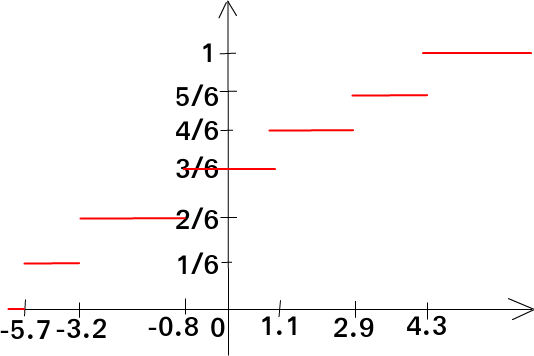
\includegraphics[width=.4\textwidth]{./pictures/1_8.png}
  \caption{Эмпирическая функция распределения}
  \label{fig:18}
\end{figure}

Выборочное среднее
$$ \overline{X} =
  \frac{1}{6} \left( -5.7 -3.2 - 0.8 + 1.1 + 2.9 + 4.3 \right) =
  \frac{1}{6} \left( -9.7 + 8.3 \right) =
  - \frac{1}{6} \cdot 1.4 =
  -0.23.$$

Выборочная дисперсия
$$ \hat{ \sigma }^2 =
  \frac{1}{5} \sum \limits_{i = 1}^6 \left( X_i + 0.23 \right)^2.$$
Она является несмещённой.

\subsubsection*{1.9}

\textit{Задание.}
Вычислите вероятность $P \left( F_n \left( y \right) < F_n \left( z \right) \right) $.

\textit{Решение.}
\begin{enumerate}[label=\alph*)]
  \item $y \geq z$.
  Событие невозможное, потому что $F_n \left( y \right) \geq F_n \left( z \right) $;
  \item рассмотрим случай, когда $y < z$.

  Тогда искомая вероятность равна
  $P \left( F_n \left( y \right) < F_n \left( z \right) \right) = P$
  \{в $ \left( y, z \right) $ попал хотя бы 1 элемент выборки\}
  $= 1 - P$\{в $ \left( y, z \right) $ ни один элемент выборки не попал\}.
  Случайные величины одинаково распределены,
  поэтому $1 - P$\{в $ \left( y, z \right) $ ни один элемент выборки не попал\} $= \\
  = \left[ 1 - P \left\{ x_i \notin \left( y, z \right) \right\} \right]^n =
  1 - \left[ 1 - P \left\{ x_1 \in \left( y, z \right) \right\} \right]^n = \\
  = 1 - \left[ 1 - P \left( x_1 < z \right) + P \left( x_1 < y \right) \right]^n =
  1 - \left[ 1 - F \left( z \right) + F \left( y \right) \right]^n$.
\end{enumerate}

\subsubsection{1.10}

\textit{Задание.} Пусть $X1, \dotsc, X_n$ --- выборка из распределения $F$ с плотностью $f$.
Найдите совместную плотность распределения всех порядковых статистик,
то есть плотность распределения случайного вектора
$ \left( X_{ \left( 1 \right) }, \dotsc, X_{ \left( n \right) } \right) $.

\textit{Решение.}
$F_{ \left( X_{ \left( 1 \right) }, X_{ \left( 2 \right) } \right) } \left( y_1, y_2 \right) =
  P \left( X_{ \left( 1 \right) } \leq y_1, \, X_{ \left( 2 \right) } \leq y_2 \right)$.
Воспользуемся формулой
$P \left( A \cap B \right) =
  P \left( B \right) - P \left( \overline{A} \cap B \right) $.
Получим
$$P \left( X_{ \left( 1 \right) } \leq y_1, \, X_{ \left( 2 \right) } \leq y_2 \right) =
  P \left( X_{ \left( 1 \right) } \leq y_2 \right) -
  P \left( X_{ \left( 1 \right) > y_1, \, X_{ \left( 2 \right) } \leq y_2} \right).$$
Среди $X_{ \left( 1 \right) }$ и $X_{ \left( 2 \right) }$ случайная величина
$X_{ \left( 2 \right) }$ является максимальной.
\begin{equation*}
  \begin{split}
    P \left( X_{ \left( 1 \right) } \leq y_2 \right) -
    P \left( X_{ \left( 1 \right) } > y_1, \, X_{ \left( 2 \right) } \leq y_2 \right) = \\
    = P \left( X_1 \leq y_2, \, X_2 \leq y_2 \right) -
    P \left( X_1 \in \left( y_1, y_2 \right], \, X_2 \in \left( y_1, y_2 \right] \right).
  \end{split}
\end{equation*}
Случайные величины $X_1, X_2$ --- независимые и одинаково распределённые
\begin{equation*}
  \begin{split}
    P \left( X_1 \leq y_2, \, X_2 \leq y_2 \right) -
    P \left( X_1 \in \left( y_1, y_2 \right], \, X_2 \in \left( y_1, y_2 \right] \right) = \\
    = \begin{cases}
      \left[ F \left( y_2 \right) \right]^2, \qquad y_1 \geq y_2, \\
      \left[ F \left( y_2 \right) \right]^2 -
      \left[ F \left( y_2 \right) - F \left( y_1 \right) \right]^2, \qquad y_1 < y_2.
    \end{cases}
\end{split}
\end{equation*}

Продифференцируем
\begin{equation*}
    f_{ \left( X_{ \left( 1 \right) }, X_{ \left( 2 \right) } \right) } \left( y_1, y_2 \right) =
    \begin{cases}
      0, \qquad y_1 \geq y_2, \\
      2f \left( y_1 \right) f \left( y_2 \right), \qquad y_1 < y_2.
    \end{cases}
\end{equation*}

Рассматриваем множество всех векторов,
которые имеют упорядоченные координаты
$ \Delta = \left\{ \vec{x} \in \mathbb{R}^n \; : \; z_1 < z_2 < \dotsc < z_n \right\}, \,
  \Gamma \subseteq \Delta $
--- произвольное подмножество.

$ \left( X_{ \left( 1 \right) }, \dotsc, X_{ \left( n \right) } \right) \in
  \Delta$.

Чтобы найти вероятность того, что данный вектор принадлежит $ \Gamma $,
должны проинтегрировать плотность этого вектора по этому множеству
$$P \left\{
    \left( X_{ \left( 1 \right) }, \dotsc, X_{ \left( n \right) } \right) \in \Gamma
  \right\} =
  \int \limits_{ \Gamma }
    f_{ \left( X_{ \left( 1 \right) }, \dotsc, X_{ \left( n \right) } \right) }
    \left( z_1, \dotsc, z_n \right)
  dz_1 \dotsc dz_n.$$

С другой стороны,
$$P \left\{
    \left( X_{ \left( 1 \right) }, \dotsc, X_{ \left( n \right) } \right) \in \Gamma
  \right\} =
  \sum \limits_{ \sigma \in S_n}
    P \left\{
      \left( X_{ \sigma \left( 1 \right) }, \dotsc, X_{ \sigma \left( n \right) } \right) \in \Gamma
    \right\}.$$
Учтём все перестановки
$$ \sum \limits_{ \sigma \in S_n}
  P \left\{
    \left( X_{ \sigma \left( 1 \right)}, \dotsc, X_{ \sigma \left( n \right) } \right) \in \Gamma
  \right\} =
  n! P \left\{ \left( X_1, \dotsc, X_n \right) \in \Gamma \right\}.$$
Подставим найденное выражение для вероятности
$$n! P \left\{ \left( X_1, \dotsc, X_n \right) \in \Gamma \right\}
  n! \cdot
  \int \limits_{ \Gamma }
    f \left( z_1 \right) \cdot \dotsc \cdot f \left( z_n \right)
  dz_1 \dotsc dz_n.$$

Сравниваем полученные выражения
$$f_{ \left( X_{ \left( 1 \right) }, \dotsc, X_{ \left( n \right) } \right) }
  \left( z_1, \dotsc, z_n \right) =
  n! f \left( z_1 \right) \cdot \dotsc \cdot f \left( z_n \right) \cdot
  \mathbbm{1} \left\{ z_1 < z_2 < \dotsc < z_n \right\}$$
--- плотность вектора упорядоченных статистик.

\subsubsection*{1.11}

\textit{Задание.}
Пусть задана выборка $X_1, \dotsc, X_n$ из показательного распределения с параметром $ \alpha $.
\begin{enumerate}[label=\alph*)]
  \item Докажите,
  что случайные величины
  $X_{ \left( 1 \right) },
    X_{ \left( 2 \right) } - X_{ \left( 1 \right) },
    \dotsc,
    X_{ \left( n \right) } - X_{ \left( n - 1 \right) }$
  являются независимыми;
  \item найдите распределение разности $X_{ \left( k + 1 \right) } - X_{ \left( k \right) }$
  соседних порядковых статистик.
\end{enumerate}

\textit{Решение.}
$ \vec{ \xi } = \left( \xi_1, \dotsc, \xi_n \right) $ ---
случайный вектор с плотностью распределения $f_{ \vec{ \xi }} \left( \vec{x} \right) $.

Линейное преобразование этого вектора $ \vec{ \eta } = A \vec{ \xi }$, где $A$ ---
некоторая $n$-мерная матрица.

$$f_{A \vec{ \xi }} \left( \vec{y} \right) =
  \frac{1}{ \left| detA \right| } \cdot f_{ \vec{ \xi }} \left( A^{-1} \vec{y} \right).$$

Составим вектор из величин
$X_{ \left( 1 \right) },
  X_{ \left( 2 \right) } - X_{ \left( 1 \right) },
  \dotsc,
  X_{ \left( n \right) } - X_{ \left( n - 1 \right) }$.
Его плотность должна распасться на произведение плотностей компонент.

Из задачи 1.10
$$f_{ \left( X_{ \left( 1 \right) }, \dotsc, X_{ \left( n \right) } \right) }
  \left( y_1, \dotsc, y_n \right) =
  n! f \left( y_1 \right) \cdot \dotsc \cdot f \left( y_n \right) \cdot
  \mathbbm{1} \left\{y_1 < y_2 < \dotsc < y_n \right\}.$$
Подставим плотность показательного распределения
\begin{equation*}
  \begin{split}
    n! f \left( y_1 \right) \cdot \dotsc \cdot f \left( y_n \right) \cdot
    \mathbbm{1} \left\{y_1 < y_2 < \dotsc < y_n \right\} = \\
    = n! \alpha e^{- \alpha y_1} \cdot \mathbbm{1} \left\{ y_1 > 0 \right\} \cdot \dotsc \cdot
    \alpha e^{- \alpha y_n} \cdot \mathbbm{1} \left\{ y_n > 0 \right\} \cdot
    \mathbbm{1} \left\{ y_1 < y_2 < \dotsc < y_n \right\}.
  \end{split}
\end{equation*}
Перемножим
\begin{equation*}
  \begin{split}
    n! \alpha e^{- \alpha y_1} \cdot \mathbbm{1} \left\{ y_1 > 0 \right\} \cdot \dotsc \cdot
    \alpha e^{- \alpha y_n} \cdot \mathbbm{1} \left\{ y_n > 0 \right\} \cdot
    \mathbbm{1} \left\{ y_1 < y_2 < \dotsc < y_n \right\} = \\
    = n! \alpha^n e^{- \alpha \left( y_1 + \dotsc + y_n \right) } \cdot
    \mathbbm{1} \left\{ 0 < y_1 < y_2 < \dotsc < y_n \right\}.
  \end{split}
\end{equation*}

Нужно найти линейное преобразование
$$\begin{bmatrix}
    X_{ \left( 1 \right) } \\
    X_{ \left( 2 \right) } - X_{ \left( 1 \right) } \\
    X_{ \left( 3 \right) } - X_{ \left( 2 \right) } \\
    \dotsc \\
    X_{ \left( n \right) } - X_{ \left( n - 1 \right) }
  \end{bmatrix} =
  \begin{bmatrix}
    1 & 0 & 0 & 9 & \dots & 0 & 0 & 0\\
    -1 & 1 & 0 & 9 & \dots & 0 & 0 & 0\\
    0 & -1 & 1 & 0 & \dotsc & 0 & 0 & 0\\
    \dotsc \\
    0 & 0 & 0 & 0 & \dotsc & 0 & -1 & 1
  \end{bmatrix}
  \begin{bmatrix}
    X_{ \left( 1 \right) )} \\
    X_{ \left( 2 \right) } \\
    X_{ \left( 3 \right) } \\
    \dotsc \\
    X_{ \left( n \right) }
  \end{bmatrix},$$
где
$$\begin{bmatrix}
    1 & 0 & 0 & 0 & \dots & 0 & 0 & 0\\
    -1 & 1 & 0 & 0 & \dots & 0 & 0 & 0\\
    0 & -1 & 1 & 0 & \dotsc & 0 & 0 & 0\\
    \dotsc \\
    0 & 0 & 0 & 0 & \dotsc & 0 & -1 & 1
  \end{bmatrix} =
  A.$$

Определитель $detA = 1$.

Ищем обратную матрицу
$$\begin{bmatrix}
    1 & 0 & 0 & 0 & \dots & 0 \\
    1 & 1 & 0 & 0 & \dots & 0 \\
    1 & 1 & 1 & 0 & \dotsc & 0 \\
    \dotsc \\
    1 & 1 & 1 & 1 & \dotsc & 1
  \end{bmatrix}
  \begin{bmatrix}
    X_{ \left( 1 \right) } \\
    X_{ \left( 2 \right) } - X_{ \left( 1 \right) } \\
    X_{ \left( 3 \right) } - X_{ \left( 2 \right) } \\
    \dotsc \\
    X_{ \left( n \right) } - X_{ \left( n - 1 \right) }
  \end{bmatrix} =
  \begin{bmatrix}
    X_{ \left( 1 \right) )} \\
    X_{ \left( 2 \right) } \\
    X_{ \left( 3 \right) } \\
    \dotsc \\
    X_{ \left( n \right) }
  \end{bmatrix}.$$

Тогда имеем выражение
$$A^{-1} \vec{y} =
  \begin{bmatrix}
    y_1 \\
    y_1 + y_2 \\
    \dotsc \\
    \sum \limits_{i = 1}^n y_i
  \end{bmatrix}.$$

Определим искомый вектор через
$$ \vec{ \eta } =
  \left(
    X_{ \left( 1 \right) },
    X_{ \left( 2 \right) } - X_{ \left( 1 \right) },
    \dotsc,
    X_{ \left(n \right) } - X_{ \left( n - 1 \right) }
  \right).$$
Тогда
\begin{equation*}
  \begin{split}
    f_{ \vec{ \eta }} \left( y_1, \dotsc, y_n \right) = \\
    = n! \alpha^n e^{- \alpha \left( ny_1 + \left( n - 1 \right) y_2 + \dotsc + y_n \right) } \cdot
    \mathbbm{1} \left\{ 0 < y_1 < y_1 + y_2 < \dotsc < y_1 + y_2 + \dotsc + y_n \right\}.
  \end{split}
\end{equation*}
Разобъём на $n$ множителей
\begin{equation*}
  \begin{split}
    n! \alpha^n e^{- \alpha \left( ny_1 + \left( n - 1 \right) y_2 + \dotsc + y_n \right) } \cdot
    \mathbbm{1} \left\{ 0 < y_1 < y_1 + y_2 < \dotsc < y_1 + y_2 + \dotsc + y_n \right\} = \\
    = \left[ n \alpha e^{- \alpha ny_1} \cdot \mathbbm{1} \left\{ 0 < y_1 \right\} \right] \cdot
    \left[
      \left( n - 1 \right) \alpha e^{- \alpha \left( n - 1 \right) y_2} \cdot
      \mathbbm{1} \left\{ y_2 > 0 \right\}
    \right] \cdot \dotsc \times \\
    \times \left[ \alpha e^{- \alpha y_n} \cdot \mathbbm{1} \left\{ y_n > 0 \right\} \right].
  \end{split}
\end{equation*}

Имеем произведение плотностей компонент, значит,
элементы вектора независимы и показательно распределены с параметром
$ \alpha \left( n - k \right) $,
то есть
$X_{ \left( k + 1 \right) } - X_{ \left( k \right) } \sim
  \Pi \left( \alpha \left( n - k \right) \right) $.
Считаем, что $X_{ \left( 0 \right) } = 0$.

\addcontentsline{toc}{section}{Домашнее задание}
\section*{Домашнее задание}

\subsubsection*{1.15}

\textit{Задание.}
Пусть $X_1, \dotsc, X_n$ ---
выборка из равномерного на отрезке $ \left[ a, b \right] $ распределения.
Вычислите математическое ожидание и дисперсию статистики
$$ \overline{X} =
  \frac{1}{n} \sum \limits_{i = 1}^n X_i.$$
Выясните, имеет ли статистика $ \overline{X}$ равномерное распределение; нормальное распределение.

\textit{Решение.} Все $X_i$ одинаково распределены.
Отсюда следует, что все математические ожидания одинаковы
$$M \overline{X} =
  \frac{1}{n} \sum \limits_{i = 1}^n MX_i =
  \frac{1}{n} \cdot nMX_1 =
  MX_1 =
  \frac{a+b}{2}.$$

Из независимости $X_i$ получаем
$$D \overline{X} =
  \frac{1}{n^2} \sum \limits_{i = 1}^n DX_i.$$

Так как $X_i$ одинаково распределены, то все дисперсии одинаковы
$$D \overline{X} =
  \frac{DX_1}{n} =
  \frac{ \left( b - a \right)^2}{12n}.$$

Чтобы выяснить,
распределена ли статистика $ \overline{X}$ по нормальному или равномерному распределению,
найдём её характеристическую функцию $ \varphi_{ \overline{X}} \left( t \right) $.
Учитывая независимость элементов выборки и то, что
$$ \varphi_{X_1} \left( t \right) =
  \dotsc =
  \varphi_{X_n} \left( t \right) =
  \frac{e^{itb} - e^{ita}}{it \left( b - a \right) },$$
находим
$$ \varphi_{ \overline{X}} \left( t \right) =
  \varphi_{X_1} \left( \frac{t}{n} \right) \cdot
  \dotsc \cdot
  \varphi_{X_n} \left( \frac{t}{n} \right) =
  \left[ \frac{\left( e^{itb} - e^{ita} \right) n}{it \left( b - a \right)} \right]^n.$$
Отсюда следует, что $ \overline{X}$ не имеет указанных распределений.

\subsubsection*{1.16}

\textit{Задание.}
Пусть $X_1, \dotsc, X_n$ --- выборка из некоторого распределения вероятностей,
функция распределения которого $F$ является непрерывной и строго возрастающей.
Найдите распределение выборки $Y_1, \dotsc, Y_n$, где
$$Y_i =
  F \left( X_i \right).$$

\textit{Решение.}
По определению
$$F_{ \eta_1, \dotsc, \eta_n} \left( X_1, \dotsc, X_n \right) =
  P \left( \eta_1 \leq X_1, \dotsc, \eta_n \leq X_n \right).$$
Воспользуемся независимостью
$$P \left( \eta_1 \leq X_1, \dotsc, \eta_n \leq X_n \right) =
  P \left( \eta_1 \leq X_1 \right) \cdot \dotsc \cdot P \left( \eta_n \leq X_n \right).$$

Функция распределения $i$-й компоненты вектора равна
$$F_{ \eta_i} \left( x \right) =
  P \left( F_{ \xi_i} \left( X_i \right) \leq x \right) =
  \begin{cases}
    0, \qquad x \leq 0, \\
    1, \qquad x > 1.
  \end{cases}$$

Рассмотрим $ \left[ 0, 1 \right] $.

Поскольку $F$ --- непрерывная и строго возрастающая, то существует $F^{-1} \left( x \right) $.
Обозначим через $z$ точку $F^{-1} \left( x \right) $ такую, что $F \left( z \right) = x$.
Событие $ \left\{ \eta = F \left( \xi \right) < x \right\} $ происходит тогда и только тогда,
когда происходит событие $ \left\{ \xi < z \right\} $.

Получаем на отрезке $ \left[ 0, 1 \right] $ равномерное распределение
$$F_{ \eta } \left( x \right) =
  F_{ \xi } \left( z \right) =
  F_{ \xi } \left( F_{ \xi }^{-1} \left( x \right) \right) =
  \begin{cases}
    0, \qquad x \leq 0, \\
    x, \qquad x \in \left( 0, 1 \right] ,\\
    1, \qquad x > 1.
  \end{cases}$$

\subsubsection*{1.17}

\textit{Задание.}
Пусть $X_1, \dotsc, X_n$ ---
выборка из дискретного распределения с вероятностями $P \left( X_1 = m \right) = p_m$, где
$$ \sum \limits_{m = 0}^N p_m =
  1.$$
Найдите распределение $k$-й порядковой статистики $X_{ \left( k \right) }$.

\textit{Решение.}
Сделали упорядочивание случайных величин
$$X_{ \left( 1 \right) } \leq
  X_{ \left( 2 \right) } \leq
  \dotsc \leq
  X_{ \left( k \right) } \leq
  \dotsc \leq
  X_{ \left( n \right)}.$$

По определению
$F_{X_{ \left( k \right) }} \left( y \right) =
  P \left( X_{ \left( k \right) } \leq y \right) =
  P$\{хотя бы $k$ элементов выборки не превышает $y$\} =
$$= \sum \limits_{i = k}^n P(A_i),$$
где $A_i =$ \{ровно $i$ элементов выборки не превышают $y$\}.

Есть $n$ испытаний, успех --- $X_i \leq y$.

Вероятность успеха --- это $F \left( y \right) $, вероятность неудачи ---
это $ \left[ 1 - F \left( y \right) \right] $.
Это биномиальное распределение
$$F_{X_{ \left( k \right) }} =
  \sum \limits_{i = k}^n
    C_n^i F^i \left( y \right) \left[ 1 - F \left( y \right) \right]^{n - i}.$$

Представим $F_{X_i} \left( y \right) = F \left( y \right) $ через $m$.
Запишем по определению
$$F_{X_1} \left( y \right) =
  P \left( X_1 \leq y \right) =
  \sum \limits_{m = 1}^n P \left( X_1 = m \right) =
  \sum \limits_{m = 1}^n p_m.$$

Подставим полученное выражение в функцию распределения
$$F_{X_{ \left( k \right) }} =
  \sum \limits_{i = k}^n
    C_n^i \sum \limits_{m = 1}^n p_m \left( 1 - \sum \limits_{m = 1}^n \right)^{n - i}.$$

\subsubsection*{1.18}

\textit{Задание.} Пусть $ \left( 3, 0, 4, 3, 6, 0, 3, 1 \right) $ --- наблюдаемые значения выборки.
Составьте вариационный ряд,
постройте эмпирическую функцию распределения $F_8 \left( x \right) $ и её график.
Вычислите выборочное среднее и выборочную дисперсию.

\textit{Решение.} Вариационный ряд: $ \left( 0, 0, 1, 3, 3, 3, 4, 6 \right) $.

Эмпирическая функция распределение (рис. \ref{fig:118})
$$F_8 \left( y \right) =
  \frac{1}{8} \sum \limits_{i = 1}^8 \mathbbm{1} \left\{ x_i \leq y \right\} =
  \begin{cases}
    0, \qquad x < 0, \\
    \frac{2}{8} = \frac{1}{4}, \qquad 0 \leq x < 1, \\
    \frac{3}{8}, \qquad 1 \leq x < 3, \\
    \frac{6}{8} = \frac{3}{4}, \qquad 3 \leq x < 4, \\
    \frac{7}{8}, \qquad 4 \leq x < 6, \\
    1, \qquad x \geq 6.
  \end{cases}$$

\begin{figure}[h!]
  \centering
  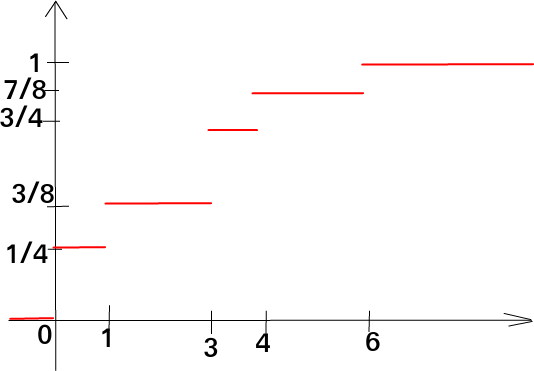
\includegraphics[width=.4\textwidth]{./pictures/1_18.png}
  \caption{Эмпирическая функция распределения}
  \label{fig:118}
\end{figure}

Выборочное среднее
$$ \overline{X} =
  \frac{1}{8} \left( 0 + 0 + 1 + 3 + 3 + 4 + 6 \right) =
  \frac{1}{8} \cdot 20 =
  \frac{10}{4} =
  2.5.$$

Выборочная дисперсия
\begin{equation*}
\begin{split}
  \hat{ \sigma^2} =
  \frac{1}{7} \sum \limits_{i = 1}^8 \left( X_i - 2.5 \right)^2 = \\
  = \frac{1}{7}
  \left[
    2 \left( 0 - 2.5 \right)^2 +
    \left( 1 - 2.5 \right)^2 +
    3 \left( 3 - 2.5 \right)^2 +
    \left( 4 - 2.5 \right)^2 +
    \left( 6 - 2.5 \right)^2
  \right] = \\
  = \frac{1}{7} \left( 12.5 + 2.25 + 0.75 + 2.25 + 12.25 \right) =
  \frac{30}{7} \approx
  4.29.
\end{split}
\end{equation*}

\addcontentsline{toc}{chapter}{Занятие 2. Свойства оценок}
\chapter*{Занятие 2. Свойства оценок}

\addcontentsline{toc}{section}{Контрольные вопросы и задания}
\section*{Контрольные вопросы и задания}

\subsubsection*{Что называют оценкой неизвестного параметра?}

Статистику, значение которой заменяет неизвестный параметр, называют оценкой этого параметра.

\subsubsection*{Приведите определение оценки: несмещённой, ассимптотически несмещённой,
                состоятельной, сильно состоятельной, оптимальной.}

Оценка $ \hat{ \theta}$  несмещённая,
если $ \forall \theta \in \Theta: \, M_{ \theta } \hat{ \theta } = \theta $.

Асимптотически несмещенная оценка --- такая оценка,
математическое ожидание которой совпадает с оцениваемым параметром при $n \to \infty $.

Оценка $ \hat{ \theta }$ называется состоятельной,
если стремится к истинному значению $ \theta $ по вероятности
$ \hat{ \theta } \overset{P}{ \rightarrow } \theta, \,
  n \to \infty $.

Оценка $ \hat{ \theta }$ называется сильно состоятельной,
если стремится к истинному значению $ \theta $ почти наверное
$ \hat{ \theta } \overset{a.s.}{ \rightarrow } \theta, \,
  n \to \infty $.

Несмещённая оценка $ \hat{ \theta } \in K$
называется оптимальной в классе квадратично интегрируемых оценок $K$,
если для всякой другой несмещённой оценки
$ \tilde{ \theta } \in \Theta \,
  \forall \theta \in \Theta: \,
  D_{ \theta } \hat{ \theta } \leq D_{ \theta } \tilde{ \theta }$
или же
$ \forall \theta \in \Theta, \,
  M_{ \theta } \left( \hat{ \theta } - \theta \right)^ \leq
  M_{ \theta } \left( \tilde{ \theta } - \theta \right)^2$.

\subsubsection*{Что называется среднеквадратическим отклонением оценки?}

$M_{ \theta } \left( \hat{ \theta } - \theta \right) $ --- среднеквадратическое оклонение.

\subsubsection*{Сформулируйте утверждение про поведение выборочных моментов.}

ыборочный начальный момент $M_k \, k$-го порядка стремится к начальному моменту $ \nu_k$
случайной величины $X$, то есть
$$ \lim \limits_{n \to \infty } P \left( \left| M_k - \nu_k \right| \geq \varepsilon \right) =
  0,$$
для любого сколь угодно малого $ \varepsilon > 0$,
если моменты $ \nu_{2k}$ и $ \nu_k$ случайной величины $X$ существуют и конечны.

\subsubsection*{Какая оценка является несмещённой и состоятельной для математического ожидания
                распределения выборки?}

В качестве оценки для математического
ожидания естественно предложить среднееарифметическое наблюденных значений
$$ \tilde{m} =
  \frac{ \sum \limits_{i = 1}^n X_i}{n}.$$

\subsubsection*{Какая статистика является несмещённой оценкой для дисперсии распределения выборки?}

$$ \frac{1}{n - 1} \sum \limits_{k = 1}^n \left( x_k - \overline{x} \right)^2$$
--- несмещённая оценка для $ \sigma^2 = Dx_1$.

\addcontentsline{toc}{section}{Аудиторные задачи}
\section*{Аудиторные задачи}

\subsubsection*{2.4}

\textit{Задание.}
Для выборки равномерного распределения на отрезке $ \left[ \theta , 1 \right] $
проверьте состоятельность и несмещённость оценки $X_{ \left( 1 \right) }$ параметра $ \theta $.

\textit{Решение.} $ \theta $ --- минимальное наблюдение.
Проверяем,
выполняется ли $X_{ \left( 1 \right) } \overset{P}{ \rightarrow } \theta, \, n \to \infty $.

По определению сходимости по вероятности
$$ \forall \varepsilon > 0 \,
  P \left( \left| X_{ \left( 1 \right) } - \theta \right| > \varepsilon \right) \to 0, \,
  n \to \infty.$$

Раскроем модуль
$$P \left\{ X_{ \left( 1 \right) } > \varepsilon + \theta \right\} =
  P \left( X_1 > \varepsilon + \theta, \dotsc, X_n > \varepsilon + \theta \right) =
  \left[ P \left( X_1 > \varepsilon + \theta \right) \right]^n.$$
Подставим значение вероятности из геометрического эксперимента
$$ \left[ P \left( X_1 > \varepsilon + \theta \right) \right]^n =
  \left( \frac{1 - \theta - \varepsilon }{1 - \theta } \right)^n =
  \left( 1 - \frac{ \varepsilon }{1 - \theta } \right)^n \to
  0, \,
  n \to \infty.$$

Число в скобках строго меньше единицы, так как $0 \leq \theta \leq 1$.

Отсюда следует, что оценка состоятельная.

Проверяем несмещённость оценки.
Проверяем, выполняется ли
$$MX_{ \left( 1 \right) } =
  \theta.$$

Нужно найти плотность
$$MX_{ \left( 1 \right) } =
  \int \limits_{ \mathbb{R}} f_{X_{ \left( 1 \right) }} \left( y \right) ydy.$$

Начинаем с функции распределения
$F_{X_{ \left( 1 \right) }} \left( y \right) =
  P \left( X_{ \left( 1 \right) } \leq y \right) $.
Переходим к противоположному событию
$$P \left( X_{ \left( 1 \right) } \leq y \right) =
  1 - P \left( X_{ \left( 1 \right) } > y \right) =
  1 - \left[ P \left( X_1 > y \right) \right]^n.$$
Переходим к противоположному событию
$1 - \left[ P \left( X_1 > y \right) \right]^n =
  1 - \left[ 1 - F \left( y \right) \right]^n$.

Продифференцируем
$$ \frac{dF_{X_{ \left( 1 \right) }} \left( y \right) }{dy} =
  n \left[ 1 - F \left( y \right) \right]^{n - 1} f \left( y \right).$$
На отрезке $ \left[ \theta, 1 \right] $ имеет равномерное распределение
$$n \left[ 1 - F \left( y \right) \right]^{n - 1} f \left( y \right) =
  n \left[ 1 - \frac{y - \theta }{1 - \theta } \right]^{n - 1} \cdot
  \mathbbm{1} \left\{ y \in \left[ \theta, 1 \right] \right\} \cdot \frac{1}{1 - \theta }.$$
Приведём к общему знаменателю
$$n \left[ 1 - \frac{y - \theta }{1 - \theta } \right]^{n - 1} \cdot
  \mathbbm{1} \left\{ y \in \left[ \theta, 1 \right] \right\} \cdot \frac{1}{1 - \theta } =
  \frac{n}{ \left( 1 - \theta \right)^2} \cdot \left( 1 - y \right)^{n - 1} \cdot
  \mathbbm{1} \left\{ y \in \left[ \theta, 1 \right] \right\}.$$

Нашли плотность $X_{ \left( 1 \right) }$ и теперь можем вычислить интеграл
$$MX_{ \left( 1 \right) } =
  \int \limits_{ \theta }^1
    y \cdot \frac{n}{ \left( 1 - \theta \right)^2} \cdot \left( 1 - y \right)^{n - 1}
  dy.$$
Замена:
$$1 - y = z, \,
  dy = -dz, \,
  y = 1 - z, \,
  y = 1 \Rightarrow \implies z = 0, \,
  y = \theta \implies z = 1 - \theta.$$
Подставляя замену, получаем
$$ \int \limits_{ \theta }^1
    y \cdot \frac{n}{ \left( 1 - \theta \right)^2} \cdot \left( 1 - y \right)^{n - 1}
  dy =
  n \cdot \frac{1}{ \left( 1 - \theta \right)^n}
  \int \limits_0^{1 - \theta } \left( 1 - z \right) z^{n - 1} dz.$$
Вычислим интеграл
\begin{equation*}
  \begin{split}
    n \cdot \frac{1}{ \left( 1 - \theta \right)^n}
    \int \limits_0^{1 - \theta } \left( 1 - z \right) z^{n - 1} dz
    \frac{n}{ \left( 1 - \theta \right)^n}
    \left[
      \frac{ \left( 1 - \theta \right)^n}{n} - \frac{ \left( 1 - \theta \right)^{n+1}}{n + 1}
    \right] = \\
    = n \left( \frac{1}{n} - \frac{1 - \theta }{n + 1} \right) =
    1 - \frac{n}{n + 1} \left( 1 - \theta \right).
  \end{split}
\end{equation*}
Раскроем скобки
$$1 - \frac{n}{n + 1} \left( 1 - \theta \right) =
  1 - \frac{n}{n + 1} - \theta \cdot \frac{n}{n + 1} \neq
  \theta.$$
Отсюда следует, что оценка смещённая, но ассимптотически несмещённая, потому что
$$1 - \frac{n}{n + 1} \to 0, \,
  n \to \infty $$
и
$$ \frac{n}{n + 1} \to 1, \,
  n \to \infty.$$

\subsubsection*{2.5}

\textit{Задание.}
Пусть $X_1, \dotsc, X_n$ --- выборка из распределения Пуассона с параметром $ \lambda > 0$.
Выясните, является ли статистика
$$ \frac{1}{n} \sum \limits_{i = 1}^n X_i^2:$$
\begin{enumerate}[label=\alph*)]
  \item несмещённой оценкой для $ \lambda^2$;
  \item состоятельной оценкой для $ \lambda^2$.
\end{enumerate}

\textit{Решение.}
\begin{enumerate}[label=\alph*)]
  \item Нужно проверить, выполняется ли
  $$M \frac{1}{n} \sum \limits_{i = 1}^n X_i^2 =
    \lambda^2.$$
  Преобразуем левую часть
  $$M \frac{1}{n} \sum \limits_{i = 1}^n X_i^2 =
    MX_1^2 =
    DX_1 + \left( MX_1 \right)^2 =
    \lambda + \lambda^2 \neq
    \lambda^2.$$

  Значит, оценка смещённая;
  \item проверяем, имеет ли место
  $$ \frac{1}{n} \sum \limits_{i = 1}^n X_i^2  \overset{P}{ \rightarrow } \lambda^2, \,
    n \to \infty.$$

  По закону больших чисел
  $$ \frac{1}{n} \sum \limits_{i = 1}^n X_i^2 \to
    MX_1^2 =
    \lambda^2 + \lambda \neq
    \lambda^2,$$
  значит, оценка не состоятельная.
\end{enumerate}

\subsubsection*{2.6}

\textit{Задание.}
Пусть $X_1, \dotsc, X_n$ --- выборка из показательного распределения с параметром $ \alpha > 0$.
Докажите, что статистика $1 / \overline{X}$ является состоятельной оценкой для $ \alpha $.

\textit{Решение.} Нужно показать, что
$$ \frac{1}{ \overline{X}} \overset{P}{ \rightarrow } \alpha, \,
   n \to \infty.$$

Выборочное среднее
$$ \overline{X} =
  \frac{1}{n} \sum \limits_{i = 1}^n X_i.$$

По закону больших чисел
$$ \overline{X} \overset{P}{ \rightarrow }
  MX_1 =
  \frac{1}{ \alpha }.$$
Отсюда следует, что
$$ \frac{1}{ \overline{X}} \overset{P}{ \rightarrow }
  \frac{1}{MX_1} =
  \alpha.$$

\subsubsection*{2.7}

\textit{Задание.}
Пусть $X_1, \dotsc, X_n$ --- выборка из нормального распределения $N \left( a, \sigma^2 \right) $.
Докажите, что статистика
$$S_n =
  \frac{1}{2 \left( n - 1 \right) } \sum \limits_{i = 1}^{n - 1} \left( X_{i + 1} - X_i \right)^2$$
является несмещённой и состоятельной оценкой для $ \sigma^1$.

\textit{Решение.} Нужно проверить условие $MS_n = \sigma^2$.

Разность двух соседних элементов выборки имеет распределение
$$X_{i + 1} - X_i \sim
  N \left( 0, 2 \sigma^2 \right).$$

Найдём математическое ожидание статистики
$$MS_n =
  M \frac{1}{2 \left( n - 1 \right) } \cdot
  \sum \limits_{i = 1}^{n - 1} \left( X_{i + 1} - X_i \right)^2 =
  \frac{1}{2 \left( n - 1 \right) } \sum \limits_{i = 1}^n M \left( X_{i + 1} - X_i \right)^2.$$
Случайные величины одинаково распределены
$$ \frac{1}{2 \left( n - 1 \right) } \sum \limits_{i = 1}^n M \left( X_{i + 1} - X_i \right)^2 =
  \frac{n}{2 \left( n - 1 \right) } \cdot M \left( X_2 - X_1 \right)^2.$$
В данном случае второй момент равен  дисперсии
$$ \frac{n}{2 \left( n - 1 \right) } \cdot M \left( X_2 - X_1 \right)^2 =
  \frac{1}{2} \cdot 2 \sigma^2 =
  \sigma^2.$$
Отсюда следует, что оценка несмещённая.

Проверим состоятельность, то есть $S_n \overset{P}{ \rightarrow } \sigma^2, \, n \to \infty $.

Разобъём $S_n$ на две суммы
$$S_n =
  \frac{1}{2 \left( n - 1 \right) } \cdot
  \left[
    \sum \limits_{even \, i} \left( X_{i + 1} - X_i \right)^2 +
    \sum \limits_{odd \, i} \left( X_{i + 1} - X_i \right)^2
  \right].$$
В каждой из сумм слагаемые независимы
\begin{equation*}
  \begin{split}
    \frac{1}{2 \left( n - 1 \right) } \cdot
    \left[
      \sum \limits_{even \, i} \left( X_{i + 1} - X_i \right)^2 +
      \sum \limits_{odd \, i} \left( X_{i + 1} - X_i \right)^2
    \right] = \\
    = \frac{1}{2 \left( n - 1 \right) } \cdot
    \left[
      \frac{m}{m} \sum \limits_{even \, i} \left( X_{i + 1} - X_i \right)^2 +
      \frac{n - 1 - m}{n - 1 - m} \sum \limits_{odd \, i} \left( X_{i + 1} - X_i \right)^2
    \right].
  \end{split}
\end{equation*}
По закону больших чисел
\begin{equation*}
  \begin{split}
    \frac{1}{2 \left( n - 1 \right) } \cdot
    \left[
      \frac{m}{m} \sum \limits_{even \, i} \left( X_{i + 1} - X_i \right)^2 +
      \frac{n - 1 - m}{n - 1 - m} \sum \limits_{odd \, i} \left( X_{i + 1} - X_i \right)^2
    \right] \overset{P}{ \rightarrow } \\
    \overset{P}{ \rightarrow } \frac{1}{2} \cdot M \left( X_2 - X_1 \right)^2 =
    \frac{1}{2} \cdot D \left( X_2 - X_1 \right) =
    \sigma^2, \,
    n \to \infty.
  \end{split}
\end{equation*}
Отсюда следует, что оценка состоятельная.

\subsubsection*{2.8}

\textit{Задание.}
Пусть $X_1, \dotsc, X_n$ --- выборка из показательного распредения с параметром $ \alpha > 1$.
Для какого параметра $ \theta = \theta \left( \alpha \right) $ статистика
$$ \hat{ \theta_n} =
  e^{ \overline{X}}$$
является состоятельной оценкой?
Является ли $ \hat{ \theta_n}$ сильно состоятельной оценкой того же параметра?
Является ли $ \hat{ \theta_n}$ несмещённой оценкой того же параметра?
Ассимптотически немещённой?

\textit{Решение.}
$$ \overline{X} =
  \frac{1}{n} \sum \limits_{i = 1}^n X_i.$$
По закону больших чисел
$$ \frac{1}{n} \sum \limits_{i = 1}^n X_i \overset{P}{ \to } MX_1, \,
  n \to \infty.$$

Случайные величины в выборке имеют показательное распределение
$$MX_1 =
  \frac{1}{ \alpha },$$
значит,
$$ \overline{X} \overset{P}{ \to } \frac{1}{ \alpha }, \,
  n \to \infty.$$

Применяем непрерывную функцию $e^x$.
Получаем $e^{ \overline{X}} \overset{P}{ \to } e^{ \frac{1}{ \alpha }}, \, n \to \infty $.

Проверяем, является ли оценка $e^{ \overline{X}}$ несмещённой к параметру $e^{ \frac{1}{ \alpha }}$,
то есть выполняется ли $Me^{ \overline{X}} = e^{ \frac{1}{ \alpha }}$.

Вычисляем $Me^{ \overline{X}} = Me^{ \frac{1}{n} \sum \limits_{i = 1}^n X_i}$.
Случайные величины независимы и одинаково распределены,
поэтому $Me^{ \frac{1}{n} \sum \limits_{i = 1}^n X_i} = \left( Me^{ \frac{X_1}{n}} \right)^n$.
По определению характеристической функции $ \varphi_{X_1} = Me^{itX_1}$ получаем
$$ \left( Me^{ \frac{X_1}{n}} \right)^n =
  \left[ \varphi_{X_1} \left( \frac{1}{in} \right) \right]^n.$$
Характеристическая функция показательного распределения
$$ \varphi_{X_1} \left(t \right) =
  Me^{itX_1} =
  \frac{ \alpha }{ \alpha - it}.$$
Подставляем
$$ \left[ \varphi_{X_1} \left( \frac{1}{in} \right) \right]^n =
  \left( \frac{ \alpha }{ \alpha - \frac{1}{n}} \right)^n.$$
Прибавим и отнимем в числителе $1 / n$ и поделим числитель на знаменатель
$$ \left( \frac{ \alpha }{ \alpha - \frac{1}{n}} \right)^n =
  \left( \frac{ \alpha + \frac{1}{n} - \frac{1}{n}}{ \alpha - \frac{1}{n}} \right)^n =
  \left[ 1 + \frac{1}{n \left( \alpha - \frac{1}{n} \right)} \right]^n =
  e^{ \frac{1}{ \alpha }}.$$
Значит, оценка смещённая, но несмещённая ассимптотически.

\subsubsection*{2.9}

\textit{Задание.}
Пусть $X_1, \dotsc, X_n$ --- выборка из геометрического распределения с параметром $p$.
Найдите состоятельные оценки для параметров
$$p, \,
  p^2, \,
  ln p, \,
  p \sin \left( 1 - p \right), \,
  pe^{ \frac{q^2}{2}}.$$

\textit{Решение.} Всё это --- непрерывные функции от $p$.
Применение непрерывной функции не нарушает сходимости по вероятности.

Если параметр каким-то образом связан со средним, но нужно пробовать выборочные моменты.

Сформируем выборочное среднее и применим закон больших чисел
$$ \overline{X} =
  \frac{1}{n} \sum \limits_{i = 1}^n X_i \overset{P}{ \to }
  MX_1.$$
Для геометрического распределения
$$MX_1 =
  \frac{1 - p}{p}.$$

Прибавим единицу слева и справа
$$1 + \overline{X} \overset{P}{ \to }
  1 + \frac{1 - p}{p} =
  1 + \frac{1}{p} - 1 =
  \frac{1}{p}.$$

Функция
$$f \left( x \right) =
  \frac{1}{x}$$
--- это непрерывная функция, значит, можем применить эту функцию слева и справа,
и сходимость сохранится
$$ \frac{1}{1 + \overline{X}} \overset{P}{ \to }
  p.$$

Состоятельной оценкой для параметра $p$ будет
$$ \hat{p} =
  \frac{1}{1 + \overline{X}}.$$

Состоятельной оценкой для $p^2$ будет $ \hat{p^2} = \hat{p}^2 \overset{P}{ \to } p^2$,
потому что $f \left( x \right) = x^2$ --- это непрерывная функция.

Логарифм --- это непрерывная функция
$$ \hat{ln p} =
  ln \hat{p} =
  ln \frac{1}{1 + \overline{X}} \overset{P}{ \to }
  ln p,$$
поскольку
$$ \frac{1}{1 + \overline{X}} \overset{P}{ \to }
  p.$$

\subsubsection*{2.12}

\textit{Задание.}
Пусть $X_1, \dotsc, X_n$ --- выборка из распределния Пуассона с параметром $ \lambda > 0$.
Докажите, что не существует несмещённой оценки для параметра $1 / \lambda $.

\textit{Решение.} Будем действовать от противного.

Допустим, что такая оценка существует, то есть существует $ \hat{ \theta }$ такое, что
$$M \hat{ \theta } =
  \frac{1}{ \lambda }.$$
Это условие несмещённости.

$ \hat{ \theta }$ --- функция от выборки,
то есть $ \hat{ \theta } = f \left( X_1, \dotsc, X_n \right) $.

Распределение Пуассона дискретное
\begin{equation*}
  \begin{split}
    M \hat{ \theta } =
    Mf \left( X_1, \dotsc, X_n \right) = \\
    = \sum \limits_{k_1 = 0}^{ \infty } \dotsc \sum \limits_{k_n = 0}^{ \infty }
      f \left( X_1, \dotsc, X_n \right) P \left( X_1 = k_1, X_2 = k_2, \dotsc, X_n = k_n \right).
  \end{split}
\end{equation*}
Воспользуемся независимостью
\begin{equation*}
  \begin{split}
    \sum \limits_{k_1 = 0}^{ \infty } \dotsc \sum \limits_{k_n = 0}^{ \infty }
      f \left( X_1, \dotsc, X_n \right) \cdot
      P \left( X_1 = k_1, X_2 = k_2, \dotsc, X_n = k_n \right) = \\
    = \sum \limits_{k_1 = 0}^{ \infty } \dotsc \sum \limits_{k_n = 0}^{ \infty }
      f \left( X_1, \dotsc, X_n \right) \cdot
      P \left( X_1 = k_1 \right) \cdot \dotsc \cdot P \left( X_n = k_n \right).
  \end{split}
\end{equation*}
Подставим в явном виде вероятности
\begin{equation*}
  \begin{split}
    \sum \limits_{k_1 = 0}^{ \infty } \dotsc \sum \limits_{k_n = 0}^{ \infty }
      f \left( X_1, \dotsc, X_n \right) \cdot
      P \left( X_1 = k_1 \right) \cdot \dotsc \cdot P \left( X_n = k_n \right) = \\
    = \sum \limits_{k_1 = 0}^{ \infty } \dotsc \sum \limits_{k_n = 0}^{ \infty }
      f \left( X_1, \dotsc, X_n \right) \cdot
      \frac{ \lambda^{ \sum \limits_{i = 1}^n k_i}}{ \prod \limits_{i = 1}^n k_i!} \cdot
      e^{- \lambda n}.
  \end{split}
\end{equation*}
Обозначим
$$ \sum k_i =
  k$$
и получим
$$e^{- \lambda n} \cdot
  \sum \limits_{k = 0}^{ \infty } \lambda^k \cdot
  \sum \limits_{k_i: \, k_1 + k_2 + \dotsc + k_n = k}
    \frac{f \left( k_1, \dotsc, k_n \right) }{k_1! \dotsc k_n!} =
  e^{- \lambda n} \sum \limits_{k = 0}^{ \infty } \lambda^k c_k,$$
где $c_k$ --- число.

Допустим, что эта величина равна $1 / \lambda $.

Посмотрим, возможно ли это
$$e^{- \lambda n} \sum \limits_{k = 0}^{ \infty } \lambda^k c_k =
  \frac{1}{ \lambda }.$$

Запишем так, чтобы с одной стороны было $e^{ \lambda n}$, а всё остальное перенесём
$$e^{ \lambda n} =
  \sum \limits_{k = 0}^{ \infty } \lambda^{k + 1} c_k.$$

Для экспоненты существует одно развитие в ряд.
Из этого следует, что последнее равенство невозможно
(развитие в ряд начинается со степени $ \lambda $, равной единице).

\addcontentsline{toc}{section}{Домашнее задание}
\section*{Домашнее задание}

\subsubsection*{2.17}

\textit{Задание.}
Пусть $X_1, \dotsc, X_n$ ---
выборка из равномерного распределения на отрезке $ \left[ 0, \theta \right] $.
Проверьте несмещённость,
состоятельность и найдите среднеквадратическое отклонение следующих оценок параметра $ \theta $:
\begin{enumerate}[label=\alph*)]
  \item $X_{ \left( 1 \right) } + X_{ \left( n \right) }$;
  \item $ \left( n + 1 \right) X_{ \left( 1 \right) }$.
\end{enumerate}

\textit{Решение.} $ \theta $ --- максимальное наблюдение.
\begin{enumerate}[label=\alph*)]
  \item Проверим,
  выполняется ли
  $X_{ \left( 1 \right) } + X_{ \left( n \right) } \overset{P}{ \to } \theta, \,
    n \to \infty $.

  По определению сходимости по вероятности
  $ \forall \varepsilon > 0 \,
    P \left( X_{ \left( 1 \right) } > \varepsilon \right) = \\
    = P \left( X_1 > \varepsilon, X_2 > \varepsilon, \dotsc, X_n > \varepsilon \right) =
    \left[ P \left( X_1 > \varepsilon \right) \right]^n.$
  Подставим значение вероятности из геометрического эксперимента
  $$ \left[ P \left( X_1 > \varepsilon \right) \right]^n =
    \left( \frac{ \theta - \varepsilon }{ \theta } \right)^n \to 0, \,
    n \to \infty.$$

  Значит, $X_{ \left( 1 \right) } \overset{P}{ \to } 0, \, n \to \infty $.

  Остаётся проверить,
  выполняется ли $X_{ \left( n \right) } \overset{P}{ \to } \theta, \, n \to \infty $.

  По определению сходимости по вероятности
  $$P \left\{ \left| X_{ \left( n \right) } - \theta \right| > \varepsilon \right\} \to 0, \,
    n \to \infty.$$

  Раскроем модуль
  \begin{equation*}
    \begin{split}
      P \left\{ \theta - X_{ \left( n \right) } > \varepsilon \right\} =
      P \left\{ X_{ \left( n \right) } - \theta < - \varepsilon \right\} =
      P \left\{ X_{ \left( n \right) } < \theta - \varepsilon \right\} = \\
      = P \left(
        X_1 < \theta - \varepsilon, X_2 < \theta - \varepsilon, \dotsc, X_n < \theta - \varepsilon
      \right) =
      \left[ P \left( X_1 < \theta - \varepsilon \right) \right]^n.
    \end{split}
  \end{equation*}
  Подставим значение вероятности из геометрического эксперимента
  $$ \left[ P \left( X_1 < \theta - \varepsilon \right) \right]^n =
    \left( \frac{ \theta - \varepsilon }{ \theta } \right)^n =
    \left( 1 - \frac{ \varepsilon }{ \theta } \right)^n \to 0, \,
    n \to \infty.$$

  Число в скобках строго меньше единицы, так как $0 \leq \theta \leq 1, \, \varepsilon > 0$.

  Отсюда следует, что оценка состоятельная.

  Проверим несмещённость оценки.
  Проверим, выполняется ли
  $$M \left( X_{ \left( 1 \right) } + X_{ \left( n \right) } \right) =
    \theta.$$

  Из задачи 1.21
  $$MX_{ \left( n \right) } =
    \frac{ \theta n}{n + 1}$$
  и
  $$MX_{ \left( 1 \right) } =
    \frac{ \theta }{n + 1}.$$
  Из свойства линейности математического ожидания
  $$M \left( X_{ \left( 1 \right) } + X_{ \left( n \right) } \right) =
    MX_{ \left( 1 \right) } + MX_{ \left( n \right) } =
    \frac{ \theta n}{n + 1} + \frac{ \theta }{n + 1} =
    \frac{ \theta \left( n + 1 \right) }{n + 1} =
    \theta.$$

  Отсюда следует, что оценка несмещённая.

  Формула среднеквадратического отклонения имеет вид $ \sigma = \sqrt{D \xi }$.

  Найдём дисперсию оценки
  \begin{equation*}
    \begin{split}
      D \left( X_{ \left( 1 \right) } + X_{ \left( n \right) } \right) =
      M \left( X_{ \left( 1 \right) } + X_{ \left( n \right) } \right)^2 -
      \left[ M \left(  X_{ \left( 1 \right) } + X_{ \left( n \right) } \right) \right]^2 = \\
      = M \left(
        X_{ \left( 1 \right) }^2 +
        X_{ \left( n \right) }^2 +
        2X_{ \left( 1 \right) } X_{ \left( n \right) }
      \right) -
      \left( MX_{ \left( 1 \right) } + MX_{ \left( n \right) } \right)^2 = \\
      = MX_{ \left( 1 \right) }^2 +
      MX_{ \left( n \right) }^2 +
      2M \left( X_{ \left( 1 \right) } X_{ \left( n \right) } \right) -
      \left( MX_{ \left( 1 \right) } \right)^2 -
      2MX_{ \left( 1 \right) } MX_{ \left( n \right) } - \\
      - \left( MX_{ \left( n \right) } \right)^2 =
      DX_{ \left( 1 \right) } +
      DX_{ \left( n \right) } +
      2cov \left( X_{ \left( 1 \right) }, X_{ \left( n \right) } \right).
    \end{split}
  \end{equation*}
  Возьмём необходимые значения из задачи 1.21, а именно
  $$DX_{ \left( 1 \right) } =
    \frac{ \theta^2 n}{ \left( n + 1 \right)^2 \left( n + 2 \right) } =
    DX_{ \left( n \right) }, \,
    cov \left( X_{ \left( 1 \right) }, X_{ \left( n \right) } \right) =
    \frac{ \theta^2}{ \left( n + 1 \right)^2 \left( n + 2 \right) }.$$
  Подставляя в найденной выражение, получаем
  \begin{equation*}
    \begin{split}
      DX_{ \left( 1 \right) } +
      DX_{ \left( n \right) } +
      2cov \left( X_{ \left( 1 \right) }, X_{ \left( n \right) } \right) = \\
      = \frac{ \theta^2 n}{ \left( n + 1 \right)^2 \left( n + 2 \right) } +
      \frac{ \theta^2 n}{ \left( n + 1 \right)^2 \left( n + 2 \right) } +
      \frac{2 \theta^2}{ \left( n + 1 \right)^2 \left( n + 2 \right) } = \\
      = \frac{2 \theta^2 n + 2 \theta }{ \left( n + 1 \right)^2 \left( n + 2 \right) } =
      \frac{2 \theta^2 \left( n + 1 \right) }{ \left( n + 1 \right)^2 \left( n + 2 \right) } =
      \frac{2 \theta^2}{ \left( n + 1 \right) \left( n + 2 \right) }.
    \end{split}
  \end{equation*}

  Извлекая корень, получаем
  $$ \sigma =
    \sqrt{ \frac{2 \theta^2}{ \left( n + 1 \right) \left( n + 2 \right) }} =
    \theta \sqrt{ \frac{2}{ \left( n + 1 \right) \left( n + 2 \right) }};$$
  \item проверим,
  выполняется ли
  $ \left( n + 1 \right) X_{ \left( 1 \right) } \overset{P}{ \to } \theta, \,
    n \to \infty $.

  По определению сходимости по вероятности
  $$ \forall \varepsilon > 0 \,
    P \left(
      \left| \left( n + 1 \right) X_{ \left( 1 \right) } - \theta \right| > \varepsilon
    \right) \to 0, \,
    n \to \infty.$$

  Перейдём к противоположному событию
  $$P \left(
    \left| \left( n + 1 \right) X_{ \left( 1 \right) } - \theta \right| > \varepsilon
  \right) =
  1 -
  P \left\{
    \left| \left( n + 1 \right) X_{ \left( 1 \right) } - \theta \right| \leq \varepsilon
  \right\}.$$
  Раскроем модуль
  \begin{equation*}
    \begin{split}
      1 - P \left\{
        \left| \left( n + 1 \right) X_{ \left( 1 \right) } - \theta \right| \leq \varepsilon
      \right\} = \\
      = 1 - P \left\{
        - \varepsilon \leq \left( n + 1 \right) X_{ \left( 1 \right) } - \theta \leq \varepsilon
      \right\} = \\
      = 1 - P \left\{
        \frac{- \varepsilon + \theta }{n + 1} \leq
        X_{ \left( 1 \right) } \leq
        \frac{ \varepsilon + \theta }{n + 1}
      \right\} = \\
      = 1 + P \left\{ X_{ \left( 1 \right) } \leq \frac{ \theta - \varepsilon }{n + 1} \right\} -
      P \left\{ X_{ \left( 1 \right) } < \frac{ \varepsilon + \theta }{n + 1} \right\} = \\
      = 1 + 1 - P \left(
        X_1 > \frac{ \theta - \varepsilon }{n + 1},
        \dotsc,
        X_n > \frac{ \theta - \varepsilon }{n + 1}
      \right) -
      1 + P \left( X_{ \left( 1 \right) } > \frac{ \varepsilon + \theta }{n + 1} \right) = \\
      = 1 - \left[ P \left( X_1 > \frac{ \theta - \varepsilon }{n + 1} \right) \right]^n +
      \left[ P \left( X_1 > \frac{ \theta + \varepsilon}{n + 1} \right) \right]^n.
    \end{split}
  \end{equation*}
  Подставим значения вероятностей из геометрического эксперимента
  \begin{equation*}
    \begin{split}
      1 - \left[ P \left( X_1 > \frac{ \theta - \varepsilon }{n + 1} \right) \right]^n +
      \left[ P \left( X_1 > \frac{ \theta + \varepsilon}{n + 1} \right) \right]^n = \\
      = 1 - \left( \frac{ \theta - \frac{ \theta - \varepsilon }{n + 1}}{ \theta } \right)^2 +
      \left( \frac{ \theta - \frac{ \varepsilon + \theta }{ n + 1}}{ \theta } \right)^n = \\
      = 1 - \left( 1 - \frac{ \theta - \varepsilon }{ \left( n + 1 \right) \theta } \right)^n +
      \left( 1 - \frac{ \varepsilon + \theta }{ \left( n + 1 \right) \theta } \right)^n \not \to
      0, \, n \to \infty.
    \end{split}
  \end{equation*}

  Отсюда следует, что оценка несостоятельная.

  Проверим несмещённость оценки.
  Проверим, выполняется ли
  $$M \left( n + 1 \right) X_{ \left( 1 \right) } =
    \theta.$$

  Выносим константу из-под знака математического ожидания
  $$ \left( n + 1 \right) MX_{ \left( 1 \right) } =
    \left( n + 1 \right) \cdot \frac{ \theta }{n + 1} =
    \theta.$$

  Отсюда следует, что оценка несмещённая.

  Найдём дисперсию оценки
  $$D \left( n + 1 \right) X_{ \left( 1 \right) } =
    \left( n + 1 \right)^2 DX_{ \left( 1 \right) } =
    \left( n + 1 \right)^2 \cdot \frac{ \theta^2 n}{ \left( n + 1 \right)^2 \left( n + 2 \right) } =
    \frac{ \theta^2 n}{n + 2},$$
  откуда среднеквадратическое отклонение равно
  $$ \sigma =
    \sqrt{D \left( n + 1 \right) X_{ \left( 1 \right) }} =
    \sqrt{ \frac{ \theta^2 n}{n + 2}} =
    \theta \sqrt{ \frac{n}{n + 2}}.$$
\end{enumerate}

\subsubsection*{2.18}

\textit{Задание.}
Пусть $X_1, \dotsc, X_n$ ---
выборка из показательного распределения с параметром $1 / \sqrt{ \alpha }$.
Выясните,
является ли статистика $ \hat{ \alpha_n} = \left( \overline{X} \right)^2$
несмещённой оценкой параметра $ \alpha $.
Является ли эта оценка состоятельной?

\textit{Решение.} Нужно проверить, выполняется ли $M \left( \overline{X} \right)^2 = \alpha $.

Запишем, что означает выборочное среднее
$$M \left( \overline{X} \right)^2 =
  M \left( \frac{1}{n} \sum \limits_{i = 1}^n X_i \right)^2 =
  M \left( \frac{1}{n^2} \left( \sum \limits_{i = 1}^n X_i \right)^2 \right) =
  \frac{1}{n^2} \cdot M \left( \sum \limits_{i = 1}^n X_i \right)^2.$$
Квадрат суммы запишем в виде двух сумм.
Получим
$$ \frac{1}{n^2} \cdot
  M \left( \sum \limits_{i = 1}^n X_i^2 + 2 \sum \limits_{k < i}^n X_k X_i \right) =
  \frac{1}{n^2} \cdot M \sum \limits_{i = 1}^n X_i +
  \frac{2}{n^2} M \sum \limits_{k < i}^n X_k X_i.$$
Случайные величины независимы и одинаково распределены, поэтому
$$ \frac{1}{n^2} \cdot M \sum \limits_{i = 1}^n X_i +
  \frac{2}{n^2} M \sum \limits_{k < i}^n X_k X_i =
  \frac{1}{n^2} \sum \limits_{i = 1}^n MX_i^2 + \frac{2}{n^2} \sum \limits_{k < i}^n MX_k MX_i.$$
Для показательного распределения
$$MX_i = \frac{1}{ \lambda } = \frac{1}{ \frac{1}{ \sqrt{ \alpha }}} = \sqrt{ \alpha }, \,
  MX_i^2 = \frac{2}{ \lambda^2} = \frac{2}{ \frac{1}{ \alpha }} = 2 \alpha.$$
Подставляем
\begin{equation*}
  \begin{split}
    \frac{1}{n^2} \sum \limits_{i = 1}^n MX_i^2 + \frac{2}{n^2} \sum \limits_{k < i}^n MX_k MX_i =
    \frac{1}{n^2} \cdot n \cdot 2 \alpha +
    \frac{1}{n^2} \cdot \left( n - 1 \right) n \left( MX_1 \right)^2 = \\
    = \frac{2 \alpha }{n} + \frac{n - 1}{n} \cdot \alpha =
    \frac{2 \alpha }{n} + \alpha - \frac{ \alpha }{n} =
    \frac{ \alpha }{n} + \alpha \to \alpha, \, n \to \infty,
  \end{split}
\end{equation*}
значит, оценка смещённая, но несмещённая ассимптотически.

Проверим, имеет ли место
$ \left( \overline{X} \right)^2 \overset{P}{ \to } \alpha, \,
  n \to \infty $.

По закону больших чисел
$$ \left( \overline{X} \right)^2 =
  \left( \frac{1}{n} \sum \limits_{i = 1}^n X_i \right)^2 \to
  \left( MX_1 \right)^2 =
  \left( \sqrt{ \alpha } \right)^2 =
  \alpha,$$
значит, оценка состоятельная.

\subsubsection*{2.21}

\textit{Задание.}
Пусть $X_1, \dotsc, X_n$ --- выборка из биномиального распределения с параметрами 2 и $p$.
Для какого параметра $ \theta = \theta \left( p \right) $ статистика
$ \hat{ \theta_n} = e^{ \overline{X}}$ будет состоятельной?
Является ли $ \hat{ \theta_n}$ сильно состоятельной оценкой того же параметра?
Является ли $ \hat{ \theta_n}$ несмещённой оценкой того же параметра?
Найдите среднеквадратическое отклонение этой оценки.

\textit{Решение.}
$$ \overline{X} =
  \frac{1}{n} \sum \limits_{i = 1}^n X_i.$$

По закону больших чисел
$$ \frac{1}{n} \sum \limits_{i = 1}^n X_i \overset{P}{ \to } MX_1, \,
  n \to \infty.$$

Случайные величины в выборке имеют биномиальное распределение с математическим ожиданием
$MX_1 = np = 2p$, значит, $ \overline{X} \overset{P}{ \to } 2p, \, n \to \infty $.

Применим непрерывную функцию $e^x$.
Получим $e^{ \overline{X}} \overset{P}{ \to } e^{2p}, \, n \to \infty $.

Проверим, является ли оценка несмещённой к параметру $e^{2p}$,
то есть выполняется ли $Me^{ \overline{X}} = e^{2p}$.

Вычисляем $Me^{ \overline{X}} = Me^{ \frac{1}{n} \sum \limits_{i = 1}^n X_i}$.
Случайные величины независимы и одинаково распределены,
поэтому $Me^{ \frac{1}{n} \sum \limits_{i = 1}^n X_i} = \left( Me^{ \frac{X_1}{n}} \right)^n$.
По определению характеристической функции $ \varphi_{X_1} \left( t \right) = Me^{itX_1}$, получим
$$ \left( Me^{ \frac{X_1}{n}} \right)^n =
  \left[ \varphi_{X_1} \left( \frac{1}{in} \right) \right]^n.$$
Характеристическая функция биномиального распределения
$$ \varphi_{X_1} \left( t \right) =
  Me^{itX_1} =
  \left[ \left( e^{it} - 1 \right) p + 1 \right]^n.$$
Подставим и получим
$$ \left[ \varphi_{X_1} \left( \frac{1}{in} \right) \right]^n =
  \left[ \left( e^{\frac{i}{in}} - 1 \right) p + 1 \right]^n =
  \left[ \left( e^{ \frac{1}{n}} - 1 \right) p + 1 \right]^n \neq
  e^{2p}.$$

Значит, оценка смещённая.

Проверим сильную состоятельность.
По усиленному закону больших чисел
$$ \overline{X} = \frac{1}{n} \sum \limits_{i = 1}^n X_i \overset{a.s.}{ \to } MX_1 = 2p, \,
  n \to \infty.$$
Отсюда следует, что $e^{ \overline{X}} \overset{a.s.}{ \to } e^{2p}, \, n \to \infty $.
Значит, оценка сильно состоятельная.

Найдём дисперсию оценки
$De^{ \overline{X}} =
  Me^{2 \overline{X}} - \left( Me^{ \overline{X}} \right)^2$.

Нашли, что $Me^{ \overline{X}} = \left[ \left( e^{ \frac{1}{n}} - 1 \right) p + 1 \right]^n$.

Вычисляем $Me^{2 \overline{X}} = Me^{ \frac{2}{n} \sum \limits_{i = 1}^n X_i}$.
Из независимости и одинаковой распределенности случайных величин следует,
что $Me^{ \frac{2}{n} \sum \limits_{i = 1}^n X_i} = \left( Me^{ \frac{2X_1}{n}} \right)^n$.
По определению характеристической функции $ \varphi_{X_1} \left( t \right) = Me^{itX_1}$, получаем
$$ \left( Me^{ \frac{2X_1}{n}} \right)^n =
  \left[ \varphi_{X_1} \left( \frac{2}{in} \right) \right]^n.$$
Подставляем характеристическую фунцию биномиального распределения
$$ \left[ \varphi_{X_1} \left( \frac{2}{in} \right) \right]^n =
  \left[ \left( e^{ \frac{2i}{in}} - 1 \right) p + 1 \right]^n =
  \left[ \left( e^{ \frac{2}{n}} - 1 \right) p + 1 \right]^n.$$
Отсюда находим дисперсию оценки
$$De^{ \overline{X}} =
  \left[ \left( e^{ \frac{2}{n}} - 1 \right) p + 1 \right]^n -
  \left[ \left( e^{ \frac{1}{n}} - 1 \right) p + 1 \right]^{2n}.$$
Извлекая корень, получим
$ \sigma =
  \sqrt{
    \left[ \left( e^{ \frac{2}{n}} - 1 \right) p + 1 \right]^n -
    \left[ \left( e^{ \frac{1}{n}} - 1 \right) p + 1 \right]^{2n}
  }.$

\subsubsection*{2.22}

\textit{Задание.} В партии из $n$ изделий оказалось $m$ бракованных.
Неизвестная вероятность $p$ появления бракованного изделия оценивается величиной $m / n$.
Проверьте состоятельность и несмещённость этой оценки.

\textit{Решение.} Выборка имеет распределение Бернулли, то есть
$$X_i =
  \begin{cases}
    1, \qquad p, \\
    0, \qquad 1 - p,
  \end{cases}$$
где событие $ \left\{ X_i = 1 \right\} $ означает, что $i$-тое изделие браковано.

Тогда
$$ \frac{m}{n} =
  \frac{X_1 + \dotsc + X_n}{n},$$
где $ \left( X_1 + \dotsc + X_n \right) $ --- количество бракованных изделий в партии.

Проверяем состоятельность, то есть проверяем, выполняется ли
$$ \frac{m}{n} \overset{p}{ \to } p, \,
  n \to \infty.$$
По закону больших чисел
$$ \frac{m}{n} =
  \frac{X_1 + \dotsc + X_n}{n} \overset{p}{ \to }
  MX_1 =
  p, \,
  n \to \infty,$$
так как это распределение Бернулли.

Это означает, что оценка состоятельная.

Проверим несмещённость оценки, то есть проверим, выполняется ли
$$M \frac{m}{n} =
  p.$$

Ищем математическое ожидание оценки
$$M \frac{m}{n} =
  M \frac{X_1 + \dotsc + X_n}{p} =
  \frac{1}{n} \cdot M \left( X_1 + \dotsc + X_n \right).$$
Пользуемся линейностью математического ожидания
$$ \frac{1}{n} \cdot M \left( X_1 + \dotsc + X_n \right) =
  \frac{1}{n} \cdot nMX_1 =
  p,$$
то есть оценка несмещённая.

\subsubsection*{2.23}

\textit{Задание.} При каком значении $k$ статистика
$$k \sum \limits_{j = 1}^n \left| X_j \right|,$$
которая построена по выборке из нормального распределения $N \left( 0, \sigma^2 \right) $,
является несмещённой оценкой для параметра $ \sigma $?

\textit{Решение.} Нужно найти такое $k$, для которого
$$M \left( k \sum \limits_{j = 1}^n \left| X_j \right| \right) =
  \sigma, \,
  X_j \sim N \left( 0, \sigma^2 \right).$$

Выносим константу $k$ за знак математического ожидания
$$M \left( k \sum \limits_{j = 1}^n \left| X_j \right| \right) =
  kM \sum \limits_{j = 1}^n \left| X_j \right|.$$
Пользуемся линейностью математического ожидания
$$kM \sum \limits_{j = 1}^n \left| X_j \right| =
  k \sum \limits_{j = 1}^n M \left| X_j \right|.$$
Из того, что случайные величины одинаково распределены, следует, что
$$k \sum \limits_{j = 1}^n M \left| X_j \right| =
  knM \left| X_1 \right|.$$

Найдём математическое ожидание модуля первого элемента выборки через плотность распределения
$$M \left| X_1 \right| =
  \int \limits_{ \mathbb{R}} p \left( x \right) \cdot \left| x \right| dx =
  \int \limits_{ \mathbb{R}}
    \left| x \right| \cdot \frac{1}{ \sqrt{2 \pi } \sigma } \cdot e^{- \frac{x^2}{2 \sigma^2}}
  dx =
  2 \cdot
  \int \limits_0^{+ \infty }
    x \cdot \frac{1}{ \sqrt{2 \pi } \sigma } \cdot e^{- \frac{x^2}{2 \sigma^2}}
  dx.$$
Внесём под знак дифференциала то, что стоит в степени экспоненты
$$2 \cdot
  \int \limits_0^{+ \infty }
    x \cdot \frac{1}{ \sqrt{2 \pi } \sigma } \cdot e^{- \frac{x^2}{2 \sigma^2}}
  dx =
  -2 \cdot \frac{1}{ \sqrt{2 \pi } \sigma } \cdot \frac{1}{2} \cdot
  \int \limits_0^{+ \infty }
    e^{- \frac{x^2}{2 \sigma^2}}
  d \left( - \frac{x^2}{2 \sigma^2} \right) \cdot
  2 \sigma^2 =
  \sqrt{ \frac{2}{ \pi }} \cdot \sigma.$$

Тогда математическое ожидание оценки
$$M \left( k \sum \limits_{j = 1}^n \left| X_j \right| \right) =
  kn \sigma \sqrt{ \frac{2}{ \pi }}$$
--- условие несмещённости, откуда
$$k =
  \frac{1}{n} \sqrt{ \frac{ \pi }{2}}.$$

\subsubsection*{2.24}

\textit{Задание.}
Пусть $X_1, \dotsc, X_n$ --- выборка из показательного распределения с параметром $ \alpha > 0$.
Найдите несмещённые состоятельные оценки для параметров
$$ \alpha, \,
  \sin \frac{1}{ \alpha }.$$

\textit{Решение.} $X_1, \dotsc, X_n$ --- независимые одинаково распределённые.

$ \theta $ --- неизвестный параметр.

$$ \hat{ \theta } =
  \frac{f \left( X_1 \right) + \dotsc + f \left( X_n \right) }{n}.$$

Так как элементы выборки одинаково распределённые, то $M \hat{ \theta } = Mf \left( X_1 \right) $.

По закону больших чисел $ \hat{ \theta } \overset{P}{ \to } Mf \left( X_1 \right) $.

Хотим, чтобы
$$ \begin{cases}
    M \hat{ \theta } = \hat{ \theta }, \\
    \hat{ \theta } \overset{P}{ \to } \theta.
  \end{cases}$$

Нужно подобрать $f$ из условия, что $Mf \left( X_1 \right) = \theta = \alpha $.

Записывая математическое ожидание через интеграл от плотности получаем преобразование Лапласа
$$ \int \limits_0^{ \infty } f \left( y \right) \alpha e^{- \alpha y} dy =
   \alpha.$$

Это способ построения одновременно несмещённой и сотоятельной оценки.

Выносим $ \alpha $ из-под знака интеграла
$$ \alpha \int \limits_0^{ \infty } f \left( y \right) e^{- \alpha y} dy =
  \alpha.$$
Сокращая константы, получаем
$$ \int \limits_0^{ \infty } f \left( y \right) e^{- \alpha y} dy =
  1.$$
Из таблицы преобразований Лапласа $f \left( y \right) = \delta \left( y \right) $.
Тогда оценка параметра $ \alpha $ примет вид
$$ \hat{ \theta } =
  \frac{ \delta \left( X_1 \right) + \dotsc + \delta \left( X_n \right) }{n}.$$

Для второго параметра
$$ \int \limits_0^{ \infty } f \left( y \right) \alpha e^{- \alpha y} dy =
  \sin \frac{1}{ \alpha }.$$

Вынесем $ \alpha $ из-под знака интеграла
$$ \alpha \int \limits_0^{ \infty } f \left( y \right) e^{- \alpha y} dy =
  \sin \frac{1}{ \alpha }.$$

Перенесём $ \alpha $ вправо
$$ \int \limits_0^{ \infty } f \left( y \right) e^{- \alpha y} dy =
  \frac{1}{ \alpha } \cdot \sin \frac{1}{y} \sim
  \frac{1}{ \alpha } \cdot \frac{1}{ \alpha } =
  \frac{1}{ \alpha^2},$$
откуда из таблицы преобразований Лапласа $f \left( y \right) = y$.
Перешли к пределу, потому что иначе интеграл расходится.
Оценка параметра в таком случае примет вид
$$ \hat{ \theta } =
  \frac{X_1 + \dotsc + X_n}{n} =
  \overline{X}.$$

\subsubsection*{2.25}

\textit{Задание.}
Пусть $X$ --- количество успехов в серии из $n$ испытаний Бернулли с вероятностью успеха $p$.
Докажите, что не существует несмещённой оценки для параметра $p^N$ при $N > n$.

\textit{Решение.} Будем действовать от противного.

Допустим, такая оценка существует, то есть существует $ \hat{ \theta }$ такое,
что $M \hat{ \theta } = p^N$.

Это условие несмещённости.

$ \hat{ \theta }$ --- функция от выборки $X_1, \dotsc, X_n$, где $X_1 + \dotsc + X_n = X$,
то есть $ \hat{ \theta } = f \left( X_1, \dotsc, X_n \right) $.

Распределение Бернулли дискретное
\begin{equation*}
  \begin{split}
    M \hat{ \theta } =
    Mf \left( X_1, \dotsc, X_n \right) = \\
    = \sum \limits_{k_1, \dotsc, k_n = 1 \, or \, 0}
      f \left( X_1, \dotsc, X_n \right) P \left( X_1 = k_1, \dotsc, X_n = k_n \right).
  \end{split}
\end{equation*}
Пользуясь независимостью, получаем
\begin{equation*}
  \begin{split}
   \sum \limits_{k_1, \dotsc, k_n = 1 \, or \, 0}
      f \left( X_1, \dotsc, X_n \right) P \left( X_1 = k_1, \dotsc, X_n = k_n \right) = \\
    = \sum \limits_{k_1, \dotsc, k_n = 1 \, or \, 0}
      f \left( X_1, \dotsc, X_n \right) \cdot
      P \left( X_1 = k_1 \right) \cdot \dotsc \cdot P \left( X_n = k_n \right).
  \end{split}
\end{equation*}
Подставляем вероятности в явном виде
\begin{equation*}
  \begin{split}
    \sum \limits_{k_1, \dotsc, k_n = 1 \, or \, 0}
      f \left( X_1, \dotsc, X_n \right) P \left( X_1 = k_1 \right) \cdot P \left( X_n = k_n \right) = \\
    = \sum \limits_{k_1, \dotsc, k_n = 1 \, or \, 0}
      f \left( X_1, \dotsc, X_n \right) p^{k_1} \cdot
      \left( 1 - p \right)^{1 - k_1} \cdot \dotsc \cdot p^{k_n} \cdot \left( 1 - p \right)^{1 - k_n} = \\
    = \sum \limits_{k_1, \dotsc, k_n = 1 \, or \, 0}
      f \left( X_1, \dotsc, X_n \right) \cdot
      p^{k_1 + \dotsc + k_n} \cdot \left( 1 - p \right)^{n - \left( k_1 + \dotsc + k_n \right) }.
    \end{split}
\end{equation*}
Обозначим
$$ \sum k_i =
  k.$$
Получим
\begin{equation*}
  \begin{split}
    \sum \limits_{k_1, \dotsc, k_n = 1 \, or \, 0}
      f \left( X_1, \dotsc, X_n \right) \cdot
      p^{k_1 + \dotsc + k_n} \cdot \left( 1 - p \right)^{n - \left( k_1 + \dotsc + k_n \right) } = \\
    = \sum \limits_{k = 0}^n
      \sum \limits_{k_1, \dotsc, k_n = 1 \, or \, 0}
        f \left( k_1, \dotsc, k_n \right) p^k \left( 1 - p \right)^{n - k} =
    \sum \limits_{k = 0}^n c_k p^k \left( 1 - p \right)^{n - k},
  \end{split}
\end{equation*}
где $c_k$ --- число.

Допустим, эта величина равна $p^N$.

Посмотрим, возможно ли это
$$ \sum \limits_{k = 0}^n c_k p^k \left( 1 - p \right)^{n - k} =
  p^N.$$

Последнее равенство невозможно при $N > n$.
Из этого следует, что не существует несмещённой оценки для параметра $p^N$ при $N > n$.

\subsubsection*{2.26}

\textit{Задание.} Проводится $n$ измерений неизвестного диаметра $d$ круга.
В первом приближении считается,
что измерения $X_i = d + \varepsilon_i$
проводятся с независимыми случайными погрешностями $ \varepsilon_i$,
которые имеют нормальное распределение с нулевым математическим ожиданием
и неизвестной дисперсией $ \sigma^2$.
Проверьте несмещённость и состоятельность следующей оценки площади круга:
$$ \hat{s_n} =
  \frac{ \pi }{4} \left( \left( \overline{X} \right)^2 - \frac{S_0^2}{n} \right),$$
где
$$S_0^2 =
  \frac{1}{n - 1} \sum \limits_{i = 1}^n \left( X_i - \overline{X} \right)^2.$$

\textit{Решение.} Имеем случайные величины $ \varepsilon_i \sim N \left( 0, \sigma^2 \right) $.
Проверим несмещённость оценки, то есть проверим, выполняется ли
$$M \hat{s_n} =
  \frac{ \pi d^2}{4}.$$

Преобразуем
$$S_0^2 =
  \frac{1}{n - 1} \sum \limits_{i = 1}^n \left( X_i - \overline{X} \right)^2 =
  \frac{1}{n - 1} \cdot
  \sum \limits_{i = 1}^n \left( d + \varepsilon_i - d - \overline{ \varepsilon } \right)^2 =
  \frac{1}{n - 1} \cdot
  \sum \limits_{i = 1}^n \left( \varepsilon_i - \overline{ \varepsilon } \right)^2.$$
Математическое ожидание этой случайной величины равно
$$MS_0^2 =
  DS_0^2 =
  \sigma^2.$$

Найдём математическое ожидание квадрата выборочного среднего
$$M \left( \overline{X} \right)^2 =
  M \left( \frac{1}{n} \sum \limits_{i = 1}^n X_i \right)^2 =
  M \left[
    \frac{1}{n^2} \cdot
    \left( \sum \limits_{i = 1}^n X_i^2 + 2 \sum \limits_{i, j = 1, \, i \neq j}^n X_i X_j \right)
  \right].$$
Пользуемся тем, что случайные величины в выборке одинаково распределены
$$M \left[
    \frac{1}{n^2} \cdot
    \left( \sum \limits_{i = 1}^n X_i^2 + 2 \sum \limits_{i, j = 1, \, i \neq j}^n X_i X_j \right)
  \right] =
  \frac{1}{n^2} \cdot nMX_1^2 + \frac{1}{n^2} \cdot 2C_n^2 \left( MX_1 \right)^2.$$
Расписываем биномиальный коэффициент
$$ \frac{1}{n^2} \cdot nMX_1^2 + \frac{1}{n^2} \cdot 2C_n^2 \left( MX_1 \right)^2 =
  \frac{1}{n} \cdot MX_1^2 +
  \frac{2}{n^2} \cdot \frac{n!}{2 \left( n - 2 \right)!} \cdot \left( MX_1 \right)^2.$$
Расписываем $n!$ через факториал, стоящий в знаменателе
$$ \frac{1}{n} \cdot MX_1^2 +
  \frac{2}{n^2} \cdot \frac{n!}{2 \left( n - 2 \right)!} \cdot \left( MX_1 \right)^2 =
  \frac{1}{n} \cdot MX_1^2 +
  \frac{2}{n^2} \cdot
  \frac{ \left( n - 2 \right)! \left( n - 1 \right) n}{2 \left( n - 2 \right)!} \cdot
  \left( MX_1 \right)^2.$$
Сокращаем
$$ \frac{1}{n} \cdot MX_1^2 +
  \frac{2}{n^2} \cdot
  \frac{ \left( n - 2 \right)! \left( n - 1 \right) n}{2 \left( n - 2 \right)!} \cdot
  \left( MX_1 \right)^2 =
  \frac{1}{n} \cdot MX_1^2 + \frac{n - 1}{n} \cdot \left( MX_1 \right)^2.$$
Найдём математическое ожидание измерения
$$MX_1 =
  M \left( d + \varepsilon_i \right) =
  Md + M \varepsilon_i =
  d.$$
Найдём математическое ожидание квадрата измерения
$$MX_1^2 =
  M \left( d + \varepsilon_i \right)^2 =
  M \left( d^2 + 2d \varepsilon_i + \varepsilon_i^2 \right) =
  Md^2 + M \left( 2d \varepsilon_i \right) + M \varepsilon_i^2.$$
Выносим константы за знак матетматического ожидания и учитываем то,
что случайная величина $ \varepsilon_i$ имеет нулевой математическое ожидание
$$Md^2 + M \left( 2d \varepsilon_i \right) + M \varepsilon_i^2 =
  d^2 + 2dM \varepsilon_i + D \varepsilon_i =
  d^2 + \sigma^2.$$
Подставляя эти значения
в полученное выражение для математического ожидания квадрата выборочного среднего, получаем
$$M \left( \overline{X} \right)^2 =
  \frac{1}{n} \cdot \left( d^2 + \sigma^2 \right) + \frac{n - 1}{n} \cdot d^2 =
  \frac{d^2 + \sigma^2 + nd^2 - d^2}{n} =
  \frac{ \sigma^2 + nd^2}{n} =
  d^2 + \frac{ \sigma^2}{n}.$$

Получаем математическое ожидание оценки
$$M \hat{s_n} =
  M \left\{
    \frac{ \pi }{4} \cdot \left[ \left( \overline{X} \right)^2 - \frac{S_0^2}{n} \right]
  \right\} =
  \frac{ \pi }{4} \cdot M \left[ \left( \overline{X} \right)^2 - \frac{S_0^2}{n} \right] =
  \frac{ \pi }{4} \cdot M \left( \overline{X} \right)^2 - \frac{ \pi }{4} \cdot M \frac{S_0^2}{n}.$$
Подставляем найденные значения математических ожиданий и выносим за скобку общий множитель
$$ \frac{ \pi }{4} \cdot M \left( \overline{X} \right)^2 - \frac{ \pi }{4} \cdot M \frac{S_0^2}{n} =
  \frac{ \pi }{4} \cdot \left( d^2 + \frac{ \sigma^2}{n} \right) - \frac{ \pi }{4n} \cdot MS_0^2 =
  \frac{ \pi }{4} \cdot d^2 + \frac{ \pi \sigma^2}{4n} - \frac{ \pi \sigma^2}{4n} =
  \frac{ \pi d^2}{4},$$
значит, оценка несмещённая.

Проверим состоятельность оценки, то есть выполняется ли
$$ \hat{s_n} \overset{P}{ \to } \frac{ \pi d^2}{4}, \,
  n \to \infty.$$

По закону больших чисел
$$ \left( \overline{X} \right)^2 \overset{P}{ \to } \left( MX_1 \right)^2 = d^2, \,
  n \to \infty.$$

Остаётся проверить, стремится ли по вероятности второе слагаемое в оценке к нулю
$$P \left( \frac{S_0^2}{n} \geq \varepsilon \right) =
  P \left( S_0^2 \geq \varepsilon n \right).$$
Применим неравенство Чебышева
$$P \left( S_0^2 \geq \varepsilon n \right) \leq
  \frac{MS_0^2}{ \varepsilon n} \to 0, \,
  n \to \infty.$$
Остюда следует, что
$$ \frac{S_0^2}{n} \overset{P}{ \to } 0, \, n \to \infty.$$
Значит,
$$ \hat{s_n} \overset{P}{ \to } \frac{ \pi }{4} \cdot d^2,$$
то есть оценка состоятельная.

\addcontentsline{toc}{chapter}{Занятие 3. Метод моментов построения оценок}
\chapter*{Занятие 3. Метод моментов построения оценок}

\addcontentsline{toc}{section}{Контрольные вопросы и задания}
\section*{Контрольные вопросы и задания}

\subsubsection*{Приведите определение оценки: несмещённой, ассимптотически несмещённой,
                состоятельной, сильно состоятельной, оптимальной.}

Оценка $ \hat{ \theta}$  несмещённая,
если $ \forall \theta \in \Theta: \, M_{ \theta } \hat{ \theta } = \theta $.

Асимптотически несмещенная оценка --- такая оценка,
математическое ожидание которой совпадает с оцениваемым параметром при $n \to \infty $.

Оценка $ \hat{ \theta }$ называется состоятельной,
если стремится к истинному значению $ \theta $ по вероятности
$ \hat{ \theta } \overset{P}{ \rightarrow } \theta, \,
  n \to \infty $.

Оценка $ \hat{ \theta }$ называется сильно состоятельной,
если стремится к истинному значению $ \theta $ почти наверное
$ \hat{ \theta } \overset{a.s.}{ \rightarrow } \theta, \,
  n \to \infty $.

Несмещённая оценка $ \hat{ \theta } \in K$
называется оптимальной в классе квадратично интегрируемых оценок $K$,
если для всякой другой несмещённой оценки
$ \tilde{ \theta } \in \Theta \,
  \forall \theta \in \Theta: \,
  D_{ \theta } \hat{ \theta } \leq D_{ \theta } \tilde{ \theta }$
или же
$ \forall \theta \in \Theta, \,
  M_{ \theta } \left( \hat{ \theta } - \theta \right)^ \leq
  M_{ \theta } \left( \tilde{ \theta } - \theta \right)^2$.

\subsubsection*{Что называется среднеквадратическим отклонением оценки?}

$M_{ \theta } \left( \hat{ \theta } - \theta \right) $ --- среднеквадратическое оклонение.

\subsubsection*{Сформулируйте утверждение про поведение выборочных моментов.}

Выборочный начальный момент $M_k \, k$-го порядка стремится к начальному моменту $ \nu_k$
случайной величины $X$, то есть
$$ \lim \limits_{n \to \infty } P \left( \left| M_k - \nu_k \right| \geq \varepsilon \right) =
  0,$$
для любого сколь угодно малого $ \varepsilon > 0$,
если моменты $ \nu_{2k}$ и $ \nu_k$ случайной величины $X$ существуют и конечны.

\subsubsection*{Сформулируйте основную идею метода моментов построения оценки
                неизвестного параметра.}

$x_1, \dotsc, x_n$ ---
выборка из распределения $F_{ \theta }$ и
$ \theta: \,
  M_{ \theta } f \left( x_1 \right) = g \left( \theta \right) $.

Вычисляем математическое ожидание, считая, что $x_1$ имеет распределение с параметром $ \theta $,
иными словами,
$$M_{ \theta } f \left( x \right) = \int \limits_{ \mathbb{R}} xdF_{ \theta } \left( x \right) , \,
  f, g \in C \left( \mathbb{R} \right), \,
  g$$
--- строго монотонная.
Тогда в силу усиленного закона больших чисел
$$ \theta \approx
  g^{-1} \left( \frac{1}{n} \sum \limits_{k = 1}^n f \left( x_k \right) \right) \overset{a.s.}
  \theta, \,
  n \to \infty.$$

Если существуют непрерывные $f$ и $g, \, g$ ---
обратима и $g \left( \theta \right) = M_{ \theta } f \left( x \right) $,
то в качестве оценки можно выбрать
$$ \hat{ \theta } =
  g^{-1} \left( \int \limits_{ \mathbb{R}} fdF_n \right).$$

\addcontentsline{toc}{section}{Аудиторные задачи}
\section*{Аудиторные задачи}

\subsubsection*{3.3}

\textit{Задание.}
Пользуясь методом моментов, оцените параметр $ \theta $ равномерного распределения на отрезке:
\begin{enumerate}[label=\alph*)]
  \item $ \left[ 0, \theta \right] $;
  \item $ \left[ \theta - 1, \theta + 1 \right] $;
  \item $ \left[ 0, 2 \theta \right] $;
  \item $ \left[ - \theta, \theta \right] $.
\end{enumerate}

\textit{Решение.}
\begin{enumerate}[label=\alph*)]
  \item $X_i \sim U \left( \left[ 0, \theta \right] \right) $.
  Записываем теоретический момент.
  Для равномерного распределения --- это средина отрезка
  $$MX_1 =
    \frac{ \theta }{2}.$$

  Должны приравнять
  $$ \frac{ \theta^*}{2} =
    \overline{X},$$
  откуда $ \theta^* = 2 \overline{X} $;
  \item случайные величины имеют распределение
  $X_i \sim
    U \left( \left[ \theta - 1, \theta + 1 \right] \right) $.

  Вычисляем теоретический момент $MX_1 = \theta $.
  Должны записать, что $ \theta^* = \overline{X}$;
  \item случайные величины имеют распределение
  $X_i \sim
    U \left( \left[ 0, 2 \theta \right] \right) $.

  Вычисляем теоретический момент $MX_1 = \theta $, откуда $ \theta^* = \overline{X}$;
  \item случайные величины имеют распределение
  $X_i \sim
    U \left( \left[ - \theta, \theta \right] \right) $.

  Вычисляем теоретический момент $MX_1 = 0$ --- не подходит,
  потому что не является функцией от $ \theta $.
  Можем вычислить второй момент, который в данном случае совпадает с дисперсией $MX_1^2 = DX_1$.
  Для равномерного распределения
  $$DX_1 =
    \frac{4 \theta^2}{12} =
    \frac{ \theta }{3}.$$
  Должны записать уравнение
  $$ \frac{ \left( \theta^2 \right)^*}{3} =
    \overline{X^2},$$
  откуда $ \left( \theta^2 \right)^* = 3 \overline{X^2}$.
  Извлекая корень, получаем $ \theta^* = \sqrt{3 \overline{X^2}}$.
\end{enumerate}

\subsubsection*{3.4}

\textit{Задание.}
Пусть $X_1, \dotsc, X_n$ --- выборка из распределения Пуассона с параметром $ \lambda $.
Пользуясь методом моментов, постройте оценку параметра $ \lambda $ и убедитесь,
что эта оценка является несмещённой и состоятельной.

\textit{Решение.} Первый теоретический момент $MX_1 = \lambda $.
Должны приравнять
$$ \lambda^* =
  \frac{1}{n} \sum \limits_{i = 1}^n X_i.$$

По закону больших чисел $ \lambda^* \overset{P}{ \to } \lambda $.
Отсюда следует состоятельность.

$M \lambda^* = MX_1 = \lambda $.
Отсюда следует несмещённость.

\subsubsection*{3.5}

\textit{Задание.} Пользуясь методом моментов с пробной функцией $g \left( y \right) = y$,
оцените параметр сдвига $ \beta \in \mathbb{R}$ показательного распределения с плотностью
$$f_{ \beta } \left( y \right) =
  \begin{cases}
    e^{ \beta - y}, \qquad t \geq \beta, \\
    0, \qquad y < \beta.
  \end{cases}$$

\textit{Решение.} $Mg \left( X_1 \right) = \overline{g \left( X \right) }$ --- метод моментов.

Ищем теоретический момент, зная плотность распределения
$$MX_1 =
  \int \limits_{ \beta }^{ \infty } ye^{ \beta - y} dy.$$
Делаем замену $y - \beta = z$ и получаем
$$ \int \limits_{ \beta }^{ \infty } ye^{ \beta - y} dy =
  \int \limits_0^{ \infty } \left( \beta + z \right) e^{-z} dz =
  \beta + 1.$$

Отсюда должны решить уравение $ \beta^* + 1 = \overline{X}$.

Отсюда $ \beta^* = \overline{X} - 1$.
Эта оценка несмещённая и состоятельная.

\subsubsection*{3.6}

\textit{Задание.}
Пусть $X_1, \dotsc, X_n$ --- выборка из биномиального распределения с параметрами $m$ и $p$.
Пользуясь методом моментов, постройте оценку:
\begin{enumerate}[label=\alph*)]
  \item параметра $p$, если параметр $m$ известный;
  \item параметра $m$, если параметр $p$ известный;
  \item векторного параметра $ \left( m, p \right) $.
\end{enumerate}

\textit{Решение.}
\begin{enumerate}[label=\alph*)]
  \item $MX_1 = mp$.
  Тогда уравенение имеет вид $mp^* = \overline{X}$.
  Отсюда
  $$p^* =
    \frac{ \overline{X}}{m};$$
  \item параметр $m$ --- это целое число.

  $m^* p = \overline{X}$, откуда
  $$m^* =
    \left[ \frac{ \overline{X}}{p} \right] $$
  --- целая часть;
  \item одного теоретического момента мало.

  Нужно найти второй теоретический момент.

  Выражаем его через дисперсию и первый момент
  $$MX_1^2 =
    DX_1 + \left( MX_1 \right)^2 =
    mp \left( 1 - p \right) + \left( mp \right)^2 =
    mp \left( 1 - p + mp \right).$$
  Составляем уравения с двумя неизвестными
  $$ \begin{cases}
      m^* p^* = \overline{X}, \\
      m^* p^* \left( 1 - p^* + m^* p^* \right) = \overline{X^2}.
    \end{cases}$$

  Во второе уравнение можем подставить $ \overline{X}$ вместо произведения $m^* p^*$ и решить
  $ \overline{X} \left( 1 - p + \overline{X} \right) = \overline{X^2}$, откуда
  $$1 - p^* + \overline{X} =
    \frac{ \overline{X^2}}{ \overline{X}}.$$

  Отсюда находим
  $$p^* =
    1 + \overline{X} - \frac{ \overline{X^2}}{ \overline{X}},$$
  соответственно
  $$m^* =
    \left[ \frac{ \overline{X}}{p^*} \right] =
    \left[ \frac{ \overline{X}}{1 + \overline{X} - \frac{ \overline{X^2}}{ \overline{X}}} \right] =
    \left[
      \frac{ \left( \overline{X} \right)^2}{ \overline{X} + \overline{X}^2 - \overline{X^2}}
    \right].$$
\end{enumerate}

\subsubsection*{3.7}

\textit{Задание.} Пусть $X_1, \dotsc, X_n$ --- выборка из распределения Парето с плотностью
$$f_{ \beta, \theta } \left( y \right) =
  \begin{cases}
    \beta \theta y^{- \left( \beta + 1 \right) }, \qquad y \geq \theta, \\
    0, \qquad t < \theta,
  \end{cases}
  \beta > 0, \,
  \theta > 0.$$

Постройте оценки по методу моментов
\begin{enumerate}[label=\alph*)]
  \item параметра $ \beta > 1$, если параметр $ \theta > 0$ известный;
  \item параметра $ \theta > 0$, если параметр $ \beta > 1$ известный;
  \item векторного параметра $ \left( \beta, \theta \right) $, где $ \beta > 2, \, \theta > 0$.
\end{enumerate}

\textit{Решение.}
\begin{enumerate}[label=\alph*)]
  \item Вычисляем теоретический момент
  $$MX_1 =
    \beta \int \limits_{ \theta }^{ \infty } \theta^{ \beta } y^{- \beta } dy =
    \beta \theta^{ \beta } \cdot \frac{y^{- \beta + 1}}{- \beta + 1} =
    - \beta \theta^{ \beta } \cdot \frac{ \theta }{1 - \beta } =
    \frac{ \beta }{ \beta - 1} \cdot \theta.$$

  Найдём второй момент
  $$MX_1^2 =
    \beta \int \limits_{ \theta }^{ \infty } \theta^{ \beta } y^{- \beta + 1} dy =
    \beta \cdot \frac{1}{ \beta - 2} \cdot \theta^2.$$

  Приравниваем теоретический и выборочный момент, учитывая, что $ \beta $ --- параметр
  $$ \frac{ \beta^*}{ \beta^* - 1} \cdot \theta =
    \overline{X},$$
  откуда
  $$ \frac{ \beta^*}{ \beta^* - 1} =
    \frac{ \overline{X}}{ \theta }.$$
  Решим пропорцию
  $ \beta^* \theta =
    \left( \beta - 1 \right) \overline{X} =
    \beta^* \overline{X} - \overline{X}$.

  Получаем
  $$ \beta^* =
    \frac{ \overline{X}}{ \overline{X} - \theta };$$
  \item считаем, что $ \beta $ --- известно, ищем $ \theta $.

  Приравниваем моменты
  $$ \frac{ \beta }{ \beta - 1} \cdot \theta =
    \overline{X},$$
  откуда
  $$ \theta^* =
    \frac{ \overline{X} \left( \beta - 1 \right) }{ \beta };$$
  \item нужно 2 уравнения
  $$ \begin{cases}
      \frac{ \beta^*}{ \beta^* - 1} \cdot \theta^* = \overline{X}, \\
      \frac{ \beta^*}{ \beta^* - 2} \cdot \left( \theta^* \right)^2 = \overline{X^2}.
    \end{cases}$$

  Выражаем $ \theta^*$ из первого уравнения и подставляем во второе
  $$ \frac{ \beta^*}{ \beta^* - 2} \cdot
    \left( \frac{ \beta^* - 1}{ \beta^*} \right)^2 \cdot
    \left( \overline{X} \right)^2 =
    \overline{X^2}.$$
  Умножим на знаменатель
  $ \left( \overline{X} \right)^2 \left( \beta^* - 1 \right)^2 =
    \overline{X^2} \beta^* \left( \beta^* - 2 \right) $.

  Оставляем в левой части только квадрат выборочного момента
  $$ \left( \overline{X} \right)^2 =
    \overline{X^2} \cdot
    \frac{ \left( \beta^* \right)^2 - 2 \beta^*}{ \left( \beta^* - 1 \right)^2}.$$

  Делаем замену $ \left( \beta^* - 1 \right)^2 = t$.

  Получаем
  $$ \left( \overline{X} \right)^2 =
    \frac{t - 1}{t} \cdot \overline{X^2} =
    \left( 1 - \frac{1}{t} \right) \cdot \overline{X^2} =
    \overline{X^2} - \frac{ \overline{X^2}}{t}.$$

  Отсюда
  $$t =
    \frac{ \overline{X^2}}{ \overline{X^2} - \left( \overline{X} \right)^2}.$$

  Отсюда найдём $ \beta^* = \sqrt{t} + 1$, соответственно находим $ \theta^*$.
\end{enumerate}

\addcontentsline{toc}{section}{Домашнее задание}
\section*{Домашнее задание}

\subsubsection*{3.10}

\textit{Задание.}
Пользуясь методом моментов,
оцените значение $ \alpha $
по выборке из показательного распределения с параметром $1 / \sqrt{ \alpha }$.

\textit{Решение.}
$$X_i \sim
  Exp \left( \frac{1}{ \sqrt{ \alpha }} \right).$$
Записываем теоретический момент.
Для показательного распределения --- это обратная величина к параметру распределения
$$MX_1 =
  \frac{1}{ \frac{1}{ \sqrt{ \alpha }}} =
  \sqrt{ \alpha }.$$

Должны приравнять $ \sqrt{ \alpha^*} = \overline{X}$,
откуда $ \alpha^* = \left( \overline{X} \right)^2$.

\subsubsection*{3.11}

\textit{Задание.}
Пусть $X_1, \dotsc, X_n$ --- выборка из показательного распределения с параметром $ \alpha > 0$.
Пользуясь методом моментов с пробной функцией $g \left( y \right) = y$,
оцените параметр $ \theta \left( \alpha \right) = P \left( X_1 > 1 \right) $.

\textit{Решение.} $Mg \left( X_1 \right) = \overline{g \left( X \right) }$ --- метод моментов.

Ищем теоретический момент, зная плотность распределения
$$MX_1 =
  \frac{1}{ \alpha }.$$
Из метода моментов следует, что
$$ \frac{1}{ \alpha^*} =
  \overline{X}.$$
Выражаем оценку
$$ \alpha^* =
  \frac{1}{ \overline{X}}.$$

Перейдём в параметре к противоположному событию
$$ \theta \left( \alpha \right) =
  P \left( X_1 > 1 \right) =
  1 - P \left( X_1 \leq 1 \right) =
  1 - F_{X_1} \left( 1 \right).$$
Найдём функцию показательного распределения как интеграл от плотности
$$F_{X_1} \left( y \right) =
  \int \limits_0^y \alpha e^{ - \alpha x} dx =
  \alpha \cdot \left( - \frac{1}{ \alpha } \right) \cdot
  \int \limits_0^{ \alpha } e^{- \alpha x} d \left( - \alpha x \right) =
  \left. -e^{- \alpha x} \right|_0^y =
  1 - e^{- \alpha y}.$$
Тогда параметр примет вид
$ \theta \left( \alpha \right) =
  1 - \left( 1 - e^{- \alpha } \right) =
  1 - 1 + e^{- \alpha } =
  e^{- \alpha } =
  e^{- \frac{1}{ \overline{X}}}.$

\subsubsection*{3.12}

\textit{Задание.}
Пользуясь методом моментов с пробной функцией $g \left( y \right) = y$,
оцените параметр $p$ распределения Бернулли.
Возможно ли с помощью метода мометов с некоторой
пробной функией $g \left( y \right) $ получить оценку параметра $p$, отличную от $ \overline{X}$?

\textit{Решение.}
$$X_i =
  \begin{cases}
    0, \qquad 1 - p, \\
    1, \qquad p.
  \end{cases}$$

Теоретический момент $MX_1 = p, \, p^* = \overline{X}$.

Найдём теоретический момент с пробной функцией
$$Mg \left( X_1 \right) =
  g \left( 0 \right) \left( 1 - p \right) + g \left( 0 \right) p =
  g \left( 0 \right) + p \left[ g \left( 1 \right) - g \left( 0 \right) \right] =
  \overline{g \left( X \right) }.$$
Отсюда
$$p^* =
  \frac{g \left( \overline{X} \right) - g \left( 0 \right) }{g \left( 1 \right) - g \left( 0 \right) }=
  \frac{g \left( X_1 \right) + \dotsc + g \left( X_n \right) - g \left( 0 \right) }{n \left[ g \left( 1 \right) - g \left( 0 \right) \right]}.$$
Количество единиц равно $ \overline{X} n$, соответственно $n - \overline{X} n$ --- количество нулей.
$$\frac{g \left( X_1 \right) + \dotsc + g \left( X_n \right) - g \left( 0 \right) }{n \left[ g \left( 1 \right) - g \left( 0 \right) \right]} =
  \frac{g \left( 1 \right) \overline{X} n + g \left( 0 \right) \left( n - \overline{X} n \right) - g \left( 0 \right) n}{n \left[ g \left( 1 \right) - g \left( 0 \right) \right] }.$$
Раскроем скобки и приведём подобные
$$ \frac{g \left( 1 \right) \overline{X} n + g \left( 0 \right) \left( n - \overline{X} n \right) - g \left( 0 \right) n}{n \left[ g \left( 1 \right) - g \left( 0 \right) \right] } =
  \frac{ng \left( 1 \right) \overline{X} - gn \overline{X}}{n \left[ g \left( 1 \right) - g \left( 0 \right) \right] } =
  \overline{X},$$
откуда следует, что невозможно получить другую оценку параметра $p$.

\subsubsection*{3.13}

\textit{Задание.}
Пользуясь методом моментов,
оцените параметр $ \lambda > 1$ по выборке из распределения Пуассона с параметром $ln \lambda $.

\textit{Решение.} Первый теоретический момент $MX_1 = ln \lambda $.
Должны приравнять $ln \lambda = \overline{X}$.
Отсюда следует, что $ \lambda^* = e^{ \overline{X}}$.

\subsubsection*{3.14}

\textit{Задание.} Пусть $X_1, \dotsc, X_n$ --- выборка из $ \Gamma $-распределения с плотностью
$$f_{ \alpha, \beta } \left( y \right) =
  \begin{cases}
    \frac{ \alpha^{ \beta }}{ \Gamma \left( \beta \right) } \cdot y^{ \beta - 1} e^{- \alpha y}, \,
    y \geq 0, \\
    0, \qquad y < 0,
  \end{cases} \,
  \alpha, \beta > 0.$$

Постройте оценки по методу моментов
\begin{enumerate}[label=\alph*)]
  \item параметра $ \alpha $, если параметр $ \beta $ известный;
  \item параметра $ \beta $, если параметр $ \alpha $ известный;
  \item векторного параметра $ \left( \alpha, \beta \right) $.
\end{enumerate}

\textit{Решение.}
\begin{enumerate}[label=\alph*)]
  \item Вычислим теоретический момент
  $$MX_1 =
    \int \limits_0^{+ \infty }
      \frac{ \alpha^{ \beta }}{ \Gamma \left( \beta \right) } \cdot
      y^{ \beta - 1} \cdot e^{- \alpha y} \cdot y
    dy =
    \frac{1}{ \Gamma \left( \beta \right) } \cdot
    \int \limits_0^{+ \infty } \alpha^{ \beta } y^{ \beta } e^{- \alpha y} dy.$$
  Сделаем замену $ \alpha y = s$, откуда
  $$y = \frac{s}{ \alpha }, \,
    dy = \frac{ds}{ \alpha }.$$
  Подставляем
  $$ \frac{1}{ \Gamma \left( \beta \right) } \cdot
    \int \limits_0^{+ \infty } \alpha^{ \beta } y^{ \beta } e^{- \alpha y} dy =
    \frac{1}{ \Gamma \left( \beta \right) } \cdot
    \int \limits_0^{+ \infty } s^{ \beta } e^{-s} \cdot \frac{ds}{ \alpha } =
    \frac{1}{ \alpha \Gamma \left( \beta \right) } \cdot
    \int \limits_0^{+ \infty } s^{ \beta } \cdot e^{-s} ds.$$
  Интеграл равен Гамма-функции
  $$ \frac{1}{ \alpha \Gamma \left( \beta \right) } \cdot
    \int \limits_0^{+ \infty } s^{ \beta } \cdot e^{-s} ds =
    \frac{1}{ \alpha \Gamma \left( \beta \right) } \cdot \Gamma \left( \beta + 1 \right) =
    \frac{1}{ \alpha \Gamma \left( \beta \right) } \cdot \beta \cdot \Gamma \left( \beta \right) =
    \frac{ \beta }{ \alpha }.$$

  Найдём второй момент
  $$MX_1^2 =
    \int \limits_0^{+ \infty }
      \frac{ \alpha^{ \beta }}{ \Gamma \left( \beta \right) } \cdot
      y^{ \beta - 1} e^{- \alpha y} \cdot y^2
    dy =
    \frac{1}{ \Gamma \left( \beta \right) } \cdot
    \int \limits_0^{+ \infty } \alpha^{ \beta } y^{ \beta + 1} e^{- \alpha y} dy.$$
  Умножаем на $ \alpha $ числитель и знаменатель
  $$ \frac{1}{ \Gamma \left( \beta \right) } \cdot
    \int \limits_0^{+ \infty } \alpha^{ \beta } y^{ \beta + 1} e^{- \alpha y} dy =
    \frac{1}{ \Gamma \left( \beta \right) \alpha } \cdot
    \int \limits_0^{+ \infty } \alpha^{ \beta + 1} y^{ \beta + 1} e^{- \alpha y} dy.$$
  Сделаем замену как и в предыдущем случае
  $$ \frac{1}{ \Gamma \left( \beta \right) \alpha } \cdot
    \int \limits_0^{+ \infty } \alpha^{ \beta + 1} y^{ \beta + 1} e^{- \alpha y} dy =
    \frac{1}{ \Gamma \left( \beta \right) \alpha^2} \cdot
    \int \limits_0^{+ \infty } s^{ \beta + 1} e^{-s} ds =
    \frac{ \Gamma \left( \beta + 2 \right) }{ \alpha^2 \Gamma \left( \beta \right) }.$$
  Пользуясь свойством Гамма-функции, записываем
  $$ \frac{ \Gamma \left( \beta + 2 \right) }{ \alpha^2 \Gamma \left( \beta \right) } =
    \frac{ \left( \beta + 1 \right) \Gamma \left( \beta + 1 \right) }{ \alpha^2 \Gamma \left( \beta \right) } =
    \frac{ \Gamma \left( \beta + 1 \right) \beta + \Gamma \left( \beta + 1 \right) }{ \alpha^2 \Gamma \left( \beta \right) }.$$
  Снова пользуемся свойством Гамма-функции и сокращаем её
  $$ \frac{ \Gamma \left( \beta + 1 \right) \beta + \Gamma \left( \beta + 1 \right) }{ \alpha^2 \Gamma \left( \beta \right) } =
    \frac{ \beta^2 \Gamma \left( \beta \right) + \beta \Gamma \left( \beta \right) }{ \alpha^2 \Gamma \left( \beta \right) } =
    \frac{ \beta^2 + \beta }{ \alpha^2}.$$

  Приравниваем теоретический момент и выборочный момент, учитывая, что $ \alpha $ --- параметр
  $$ \frac{ \beta }{ \alpha^*} =
    \overline{X},$$
  откуда
  $$ \alpha^* =
    \frac{ \beta }{ \overline{X}};$$
  \item считаем, что $ \alpha $ --- известно, ищем $ \beta^*$.

  Приравниваем моменты
  $$ \frac{ \beta^*}{ \alpha } =
    \overline{X},$$
  откуда $ \beta^* = \alpha \overline{X}$;
  \item нужно 2 уравнения
  $$ \begin{cases}
      \frac{ \beta^*}{ \alpha^*} = \overline{X}, \\
      \frac{ \left( \beta^* \right)^2 + \beta^*}{ \left( \alpha^* \right)^2} = \overline{X^2}.
    \end{cases}$$

  Выражаем $ \alpha^*$ из первого уравнения и подставляем во второе
  $$ \frac{ \left( \beta^* \right)^2 + \beta^*}{ \beta^*} \cdot \overline{X} =
    \overline{X^2}.$$

  Поделим числитель на знаменатель
  $$ \left( 1 + \frac{1}{ \beta^*} \right) \cdot \left( \overline{X} \right)^2 =
    \overline{X^2}.$$
  Оставляем в левой части только скобку
  $$ 1 + \frac{1}{ \beta^*} =
    \frac{ \overline{X^2}}{ \left( \overline{X} \right)^2}.$$

  Переносим единицу вправо
  $$ \frac{1}{ \beta^*} =
    \frac{ \overline{X^2}}{ \left( \overline{X} \right)^2} - 1.$$
  Выражаем параметр
  $$ \beta^* =
    \frac{1}{ \frac{ \overline{X^2}}{ \left( \overline{X} \right)^2} - 1} =
    \frac{ \left( \overline{X} \right)^2}{ \overline{X^2} - \left( \overline{X} \right)^2}.$$

  Соответственно находим
  $$ \alpha^* =
    \frac{ \beta^*}{ \overline{X}} =
    \frac{ \frac{ \left( \overline{X} \right)^2}{ \overline{X^2} - \left( \overline{X} \right)^2}}{ \overline{X}} =
    \frac{ \left( \overline{X} \right)^2}{ \left( \overline{X^2} - \left( \overline{X} \right)^2 \right) \overline{X}} =
    \frac{ \overline{X}}{ \overline{X^2} - \left( \overline{X} \right)^2о }.$$
\end{enumerate}

\subsubsection*{3.15}

\textit{Задание.}
Пусть $X_1, \dotsc, X_n$ --- выборка из биномиального распределения с параметрами $2, \, p$.
Пользуясь методом моментов с пробной функцией
$$g \left( y \right) = y,$$
оцените параметр $ \theta = e^{2p}$.

\textit{Решение.} $Mg \left( X_1 \right) = \overline{g \left( X \right) }$ --- метод моментов.

Ищем теоретический момент, зная распределение
$$MX_1 =
  \sum \limits_{k = 0}^2 k \cdot P \left( X_1 = k \right) =
  \sum \limits_{k = 0}^2 k \cdot C_2^k p^k \left( 1 - p \right)^{2 - k}.$$
При $k = 0$ первое слагаемое зануляется, поэтому можно суммировать от единицы
$$ \sum \limits_{k = 0}^2 k \cdot C_2^k p^k \left( 1 - p \right)^{2 - k} =
  \sum \limits_{k = 1}^2 k \cdot C_2^k \cdot p^k \left( 1 - p \right)^{2 - k} =
  1 \cdot C_2^1 p \left( 1 - p \right) + 2 \cdot C_2^2 \cdot p^2.$$
Распишем биномиальные коэффициенты, раскроем скобки и приведём подобные
$$1 \cdot C_2^1 p \left( 1 - p \right) + 2 \cdot C_2^2 \cdot p^2 =
  2p \left( 1 - p \right) + 2p^2 =
  2p - 2p^2 + 2p^2 =
  2p.$$

Должны решить уравнение $2p^* = \overline{X}$.

Отсюда
$$p^* =
  \frac{ \overline{X}}{2}.$$

Оценим параметр $ \theta^* = e^{2p^*} = e^{ \frac{2 \overline{X}}{2}} = e^{ \overline{X}}$.

\addcontentsline{toc}{chapter}{Занятие 4. Оценка максимального правдоподобия}
\chapter*{Занятие 4. Оценка максимального правдоподобия}

\addcontentsline{toc}{section}{Контрольные вопросы и задания}
\section*{Контрольные вопросы и задания}

\subsubsection*{Как построить оценку максимального правдоподобия?}

Плотность распределения выборки $\left( X_1, \dotsc, X_n \right) $ имеет вид
$$L \left( \vec{X}, \theta \right) =
  \prod \limits_{k = 1}^n p \left( X_k, \theta \right),$$
как плотность вектора с независимыми координатами.
$L \left( \vec{X}, \theta \right) $ --- функция правдоподобия.

Оценка максимаьлного правдоподобия $ \hat{ \theta }$ --- такое значение параметра $ \theta $,
при котором функция правдоподобия достикает своего максимального значения
$ \hat{ \theta } =
  \underset{ \theta }{argmax} L \left( \vec{X}, \theta \right) $.

\subsubsection*{Сформулируйте свойства оценки максимального правдоподобия.}

Оценка максимального правдоподобия, как правило, сильно состоятельная.

\addcontentsline{toc}{section}{Аудиторные задачи}
\section*{Аудиторные задачи}

\subsubsection*{4.3}

\textit{Задание.}
Постройте оценку максимального правдоподобия векторного параметра $ \left( a, \sigma^2 \right) $
нормального распределения.

\textit{Решение.} Выборка $x_1, \dotsc, x_n \sim N \left( a, \sigma^2 \right) $.
Сейчас $ \theta $ будет векторным параметром, состоящим из двух элементов: $a, \sigma^2$.

Плотность имеет вид
$$p \left( x \right) =
  \frac{1}{ \sqrt{2 \pi } \sigma } \cdot e^{- \frac{ \left( x - a \right)^2}{2 \sigma^2}}.$$

Произведение этих плотностей даёт
$$L \left( \vec{x}, a, \sigma^2 \right) =
  \frac{1}{ \left( 2 \pi \right)^{ \frac{n}{2}} \sigma^n}
  \cdot e^{- \frac{1}{2 \sigma^n} \cdot \sum \limits_{i = 1}^n \left( x_i - a \right)^2}.$$
Обозначим $ \sigma^2 = \sigma^*$, чтобы было удобней брать производную
$$ \frac{1}{ \left( 2 \pi \right)^{ \frac{n}{2}} \sigma^2}
  \cdot e^{- \frac{1}{2 \sigma^2} \cdot \sum \limits_{i = 1}^n \left( x_i - a \right)^2} =
  \frac{1}{ \left( 2 \pi \right)^{ \frac{n}{2}} \left( \sigma^* \right)^{ \frac{n}{2}}} \cdot
  e^{- \frac{1}{2 \sigma^*} \cdot \sum \limits_{i = 1}^n \left( x_i - a \right)^2}.$$

Поскольку есть экспонента, стоит брать логарифм
$$l \left( \vec{x}, a, \sigma^* \right) =
  ln L \left( \vec{x}, a, \sigma^* \right) =
  - \frac{n}{2} \cdot ln \left( 2 \pi \sigma^* \right) -
  \frac{1}{2 \sigma^*} \sum \limits_{i = 1}^n \left( x_i - a \right)^2.$$
Распишем логарифм произведения через сумму логарифмов
$$- \frac{n}{2} \cdot ln \left( 2 \pi \sigma^* \right) -
  \frac{1}{2 \sigma^*} \sum \limits_{i = 1}^n \left( x_i - a \right)^2 =
  - \frac{n}{2} \cdot ln \left( 2 \pi \right) -
  \frac{n}{2} \cdot ln \sigma^* -
  \frac{1}{2 \sigma^*} \sum \limits_{i = 1}^n \left( x_i - a \right)^2.$$

Берём производную
$$ \frac{ \partial }{ \partial \sigma^*} l =
  - \frac{n}{2} \cdot \frac{1}{ \sigma^*} +
  \frac{1}{2 \left( \sigma^* \right)^2} \sum \limits_{i = 1}^n \left( x_i - a \right)^2 =
  0.$$

Теперь надо по $a$ продифференцировать и тоже приравнять к нулю
$$ \frac{ \partial }{ \partial a} l =
  \frac{1}{ \sigma^*} \sum \limits_{i = 1}^n \left( x_i - a \right) =
  0 =
  \frac{n \overline{X} - na}{ \sigma^*}.$$

Распишем сумму в явном виде
$ \left( x_1 - a \right) + \left( x_2 - a \right) + \dotsc + \left( x_n - a \right) =
  0$.

Отсюда
$$a =
  \frac{1}{n} \sum \limits_{i = 1}^n x_i.$$

Оценка равна $ \hat{a} = \overline{x}.$

Тогда оценка второго параметра равна
$$ \hat{ \sigma^*} =
  \frac{1}{n} \sum \limits_{i = 1}^n \left( x_i - \overline{x} \right)^2.$$

Проверили только необходимое условие для максимума.
Теперь нужно проверить достаточность.

Имеем матрицу $n \times n$.
Матрица положительно определена тогда и только тогда, когда каждый минор положительный.
Матрица отрицательно определена тогда и только тогда, когда каждый минор отрицательный.

$$ \begin{bmatrix}
  \frac{ \partial^2}{ \partial a^2} & \frac{ \partial^2}{ \partial a \partial \sigma^*} \\
  \frac{ \partial^2}{ \partial a \partial \sigma^*} & \frac{ \partial^2}{ \partial \left( \sigma^* \right)^2}
\end{bmatrix}.$$

Найдём последний элемент матрицы
$$ \frac{ \partial^2}{ \partial \left( \sigma^* \right)^2} l =
  \frac{n}{2 \left( \sigma^* \right)^2} -
  \frac{1}{ \left( \sigma^* \right)^3} \cdot \sum \limits_{i = 1}^n \left( x_i - a \right)^2.$$

Найдём смешанную производную
$$ \frac{ \partial^2}{ \partial a \partial \sigma^*} l =
  - \sum \limits_{i = 1}^n \left( x_i - a \right) \cdot \frac{1}{ \left( \sigma^* \right)^2} =
  \frac{n \overline{x} - na}{ \left( \sigma^* \right)^2}.$$

Найдём первый элемент матрицы
$$ \frac{ \partial^2}{ \partial a^2} l =
  - \frac{n}{ \sigma^*}.$$

Теорема Шварца.
Если
$$ \exists \frac{ \partial^2 f}{ \partial x \partial y}, \,
  \frac{ \partial^2 f}{ \partial y \partial x}$$
и они непрерывны в точке $ \left( x_0, y_0 \right) $, то они совпадают в этой точке.

Первый определитель строго отрицательный.

Второй определитель
$$M_2 =
  - \frac{n^2}{2 \left( \sigma^* \right)^3} +
  \frac{n}{ \left( \sigma^* \right)^4} \cdot \sum \limits_{i = 1}^n \left( x_i - a \right) -
  \frac{n}{ \left( \sigma^* \right)^4} \cdot \left( \overline{x} - a \right)^2.$$
Последнее слагаемое равно нулю.
Нужно проверять это значение в точке $ \hat{a} = \overline{x}$.
Имеем
\begin{equation*}
  \begin{split}
    - \frac{n^2}{2 \left( \sigma^* \right)^3} +
    \frac{n}{ \left( \sigma^* \right)^4} \cdot \sum \limits_{i = 1}^n \left( x_i - a \right) -
    \frac{n}{ \left( \sigma^* \right)^4} \cdot \left( \overline{x} - a \right)^2 = \\
    = - \frac{n}{ \left( \sigma^* \right)^3} \cdot
    \left( \frac{n}{2} - \frac{1}{ \sigma^*} \cdot
    \sum \limits_{i = 1}^n \left( x_i - a \right) \right) >
    0.
  \end{split}
\end{equation*}

Нужно проверить в точке $ \sigma^* = \hat{ \sigma }$.
Имеем
$$ \frac{n}{2} <
  \frac{ \sum \limits_{i = 1}^n \left( x_i - a \right)^2}{ \sigma^*}.$$

Отсюда выражаем значение оценки
$$ \sigma^* =
  \hat{ \sigma } =
  \frac{1}{n} \sum \limits_{i = 1}^n \left( x_i - \overline{x} \right).$$
Следовательно,
$$ \frac{n}{2} < n,$$
то есть $M_2 < 0$.
По критерию Сильвестра $ \hat{A} < 0$ тогда и только тогда,
когда $ \left( \hat{a}, \hat{ \sigma^*} \right) $ --- точка максимума.

\subsubsection*{4.5}

\textit{Задание.}
Постройте оценку максимального правдоподобия параметра $ \theta $ показательного распределения.

\textit{Решение.}
$p \left( x, \theta \right) =
  \theta e^{- \theta x} \cdot \mathbbm{1} \left\{ x \geq 0 \right\} $.

Нужно найти функцию правдобоподия как произведение плотностей
$L \left( \vec{x}, \theta \right) =
  \theta^n \cdot e^{-n \theta \sum \limits_{i = 1}^n x_i} \cdot
  \mathbbm{1} \left\{ \vec{x} \in \left[ 0, + \infty \right)^n \right\} $.
Предполагаем, что все $x_i \geq 0$, то есть индикатор можно отбросить.
Если какой-то элемент выборки сильно отрицательный,
то не имеет смысла говорить о равномерном распределении.
Если какой-то элемент выборки близок к нулю и при этом отрицательный, то на него повлияла ошибка,
и его не учитываем
$$ \theta^n \cdot e^{-n \theta \sum \limits_{i = 1}^n x_i} \cdot
  \mathbbm{1} \left\{ \vec{x} \in \left[ 0, + \infty \right)^n \right\} =
  \theta^n e^{-n \theta \sum \limits_{i = 1}^n x_i}.$$

Удобнее будет рассмотреть
$$ln L \left( \vec{x}, \theta \right) =
  l \left( \theta \right) =
  - \theta \sum \limits_{i = 1}^n x_i + n ln \theta.$$

Нужно взять производную и приравнять к нулю
$$ \frac{ \partial }{ \partial \theta } l \left( \theta \right) =
  - \sum \limits_{i = 1}^n x_i + \frac{n}{ \theta } =
  0.$$

Переносим сумму вправо
$$ \frac{n}{ \theta } =
  \sum \limits_{i = 1}^n x_i.$$

Получаем оценку
$$ \hat{ \theta } =
  \frac{n}{ \sum \limits_{i = 1}^n x_i}.$$
Выразим через выборочное среднее
$$ \frac{n}{ \sum \limits_{i = 1}^n x_i} =
  \frac{1}{ \overline{X}}.$$
Остаётся проверить, что $ \hat{ \theta }$ будет действительно максимумом функции $l$.
Нужно найти вторую производную
$$ \frac{ \partial^2}{ \partial \theta^2} l \left( \theta \right) =
  - \frac{n}{ \theta^n} <
  0.$$
Отсюда следует, что фунция выпуклая ввекх, соответственно это точка максимума.

\subsubsection*{4.6}

\textit{Задание.}
Постройте оценку максимального правдоподобия параметра $ \theta > 0$
равномерного распределения на отрезке $ \left[ 0, \theta \right] $.

\textit{Решение.}
Плотность равномерного распределения на отрезке $ \left[ 0, \theta \right] $ имеет вид
$$p_{ \theta } \left( x \right) =
  \frac{ \mathbbm{1} \left\{ x \in \left[ 0, \theta \right] \right\} }{ \theta }.$$
По этой плотности строим функцию правдоподобия
$$L \left( \vec{x}, \theta \right) =
  \frac{ \mathbbm{1} \left\{ \vec{x} \in \left[ 0, \theta \right]^n \right\} }{ \theta^n} =
  \frac{ \mathbbm{1} \left\{ \min \limits_i x_i \geq 0, \, \max \limits_i x_i \leq \theta \right\} }{ \theta^n}.$$
Если какой-то элемент выборки сильно отрицательный,
то не имеет смысла говорить о равномерном распределении, если близок к нулю,
то на него повлияла ошибка, и его не учитываем
$$ \frac{ \mathbbm{1} \left\{ \min \limits_i x_i \geq 0, \, \max \limits_i x_i \leq \theta \right\} }{ \theta^n} =
  \frac{ \mathbbm{1} \left\{ \max \limits_i x_i \leq \theta \right\} }{ \theta }.$$

Нарисуем график получившейся функции как функции от $ \theta $ (рис. \ref{fig:46}).

\begin{figure}[h!]
  \centering
  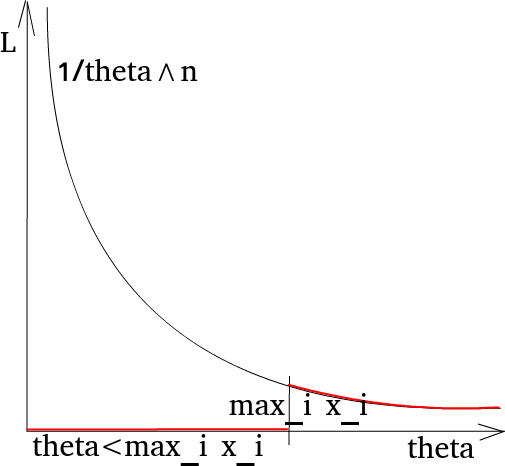
\includegraphics[width=.4\textwidth]{./pictures/4_6.png}
  \caption{График функции $L \left( \theta \right) $}
  \label{fig:46}
\end{figure}

Точка максимума такой функции --- это $ \max \limits_i x_i$.

Значит, $ \hat{ \theta } = \max \limits_{1 \leq i \leq n} x_i$.

\subsubsection*{4.7}

\textit{Задание.}
Постройте оценку максимального правдоподобия параметра сдвига $ \beta \in \mathbb{R}$
показательного распределения с плотностью
$$f_{ \beta } \left( y \right) =
  \begin{cases}
    e^{ \beta - y}, \qquad y \geq \beta, \\
    0, \qquad otherwise.
  \end{cases}$$

Проверьте состоятельность этой оценки.

\textit{Решение.}
$f_{ \beta } \left( y \right) = e^{ \beta - y} \cdot \mathbbm{1} \left\{ y \geq \beta \right\}.$

Запишем функцию правдоподобия
$$L \left( \vec{x}, \beta \right) =
  e^{n \beta - \sum \limits_{i = 1}^n x_i} \cdot
  \mathbbm{1} \left\{ \vec{x} \in \left[ \beta, + \infty \right)^n \right\} =
  e^{n \beta - \sum \limits_{i = 1}^n x_i} \cdot
  \mathbbm{1} \left\{ \min \limits_{1 \leq i \leq n} x_i \geq \beta \right\}.$$
Рисуем схематический график (рис. \ref{fig:47}).

\begin{figure}[h!]
  \centering
  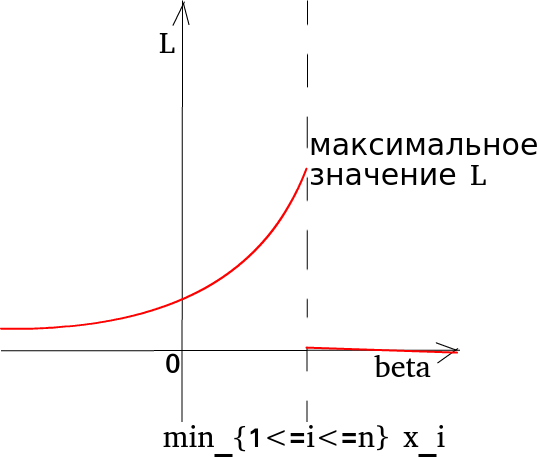
\includegraphics[width=.4\textwidth]{./pictures/4_7.png}
  \caption{График функции $L \left( \beta \right) $}
  \label{fig:47}
\end{figure}

Из графика видно, что $ \hat{ \beta } = \min \limits_{1 \leq i \leq n} x_i$.
Проверяем состоятельность:
$$ \hat{ \beta } \overset{P}{ \to } \beta, \, n \to \infty.$$
По определению
$P \left( \left| \hat{ \beta } - \beta \right| > \varepsilon \right) \to 0,
  \, n \to \infty, \,
  \forall \varepsilon > 0$.
Подставляем оценку в функцию правдоподобия
$$e^{n \beta - \sum \limits_{i = 1}^n x_i} \cdot
  \mathbbm{1} \left\{ \min \limits_{1 \leq i \leq n} x_i \geq \beta \right\} =
  P \left( \left| \min \limits_{1 \leq i \leq n} x_i - \beta \right| > \varepsilon \right).$$
Минимальный член выборки не может быть меньше $ \beta $ из-за распределения.
$P \left( \left| \min \limits_{1 \leq i \leq n} x_i - \beta \right| > \varepsilon \right) =
  P \left( \min \limits_{1 \leq i \leq n} x_i > \beta + \varepsilon \right).$
Запишем через вероятность пересечения событий $ \left\{ x_i > \beta + \varepsilon \right\} $.
Получим
$$P \left( \min \limits_{1 \leq i \leq n} x_i > \beta + \varepsilon \right) =
  P \left( \bigcap \limits_{i = 1}^n \left\{ x_i > \beta + \varepsilon \right\} \right).$$
Случайные величины независимы и одинаково распределены
$$P \left( \bigcap \limits_{i = 1}^n \left\{ x_i > \beta + \varepsilon \right\} \right) =
  \left[ P \left( x_1 > \beta + \varepsilon \right) \right]^n \to 0, \,
  n \to \infty,$$
так как такая вероятность меньше единицы.

Достаточно показать, что $P \left( x_1 > \beta + \varepsilon \right) \neq 1$.
Тогда $l^n \to 0$.

Запишем интеграл от плотности со сдвигом
$$ \int \limits_{ \beta + \varepsilon }^{+ \infty } p_{ \beta } \left( y \right) dy =
  1 - \int \limits_{ \beta }^{ \beta + \varepsilon } p_{ \beta } \left( y \right) dy <
  1,$$
так как второй интеграл больше нуля (забрали кусок $ \beta + \varepsilon $).

\subsubsection*{4.8}

\textit{Задание.}
Постройте оценку максимального правдоподобия параметра сдвига $ \mu \in \mathbb{R}$
распределения Лапласа с плотностью
$f_{ \mu } \left( y \right) =
  e^{- \frac{ \left| y - \mu \right| }{2}}$.

\textit{Решение.} Записываем функцию правдоподобия
$$L \left( \vec{X}, \mu \right) =
  \prod \limits_{i = 1}^n f_{ \mu } \left( X_i \right) =
  \prod \limits_{i = 1}^n \frac{1}{2} \cdot e^{- \left| X_i - \mu \right| } =
  \frac{1}{2^n} \cdot e^{- \sum \limits_{i = 1}^n \left| X_i - \mu \right| }.$$

Находим  логарифм
$$l \left( \vec{X}, \mu \right) =
  c - \sum \limits_{i = 1}^n \left| X_i - \mu \right|,$$
где $c = const$.
Дифференцировать по $ \mu $ не можем.
Хотим максимизировать эту функцию правдоподобия.
Нужно минимизировать сумму $X_i$ --- точки на оси.
$ \left| X_i - \mu \right| $ --- расстояние.

Вариационный ряд имеет понятие медианы.
Это приблизительно средина вариационного ряда.

$$ \mu^* =
  \begin{cases}
    X_{ \left( m + 1 \right) }, \qquad n = 2m + 1, \\
    \frac{X_{ \left( m \right) + X_{ \left( m + 1 \right) }}}{2}, \qquad n = 2m
  \end{cases}$$
--- аналогия с центром масс треугольника, который задаётся как точка пересечения медиан.

\subsubsection*{4.9}

\textit{Задание.} Постройте оценку максимального правдоподобия параметра $p$ распределения Бернулли.

\textit{Решение.} Распределение Бернулли не имеет плотности.
Есть выборка $x_1, \dotsc, x_n \sim B \left( 1, p \right) $.

Сформулируем метод максимального правдоподобия в общем случае.

$X_1, \dotsc, X_n$ --- выборка с параметром $ \theta $.

$X_1, \dotsc, X_n$ имеют плотность распределения $p_{ \theta } \left( y \right) $.
Тогда
$$L \left( \vec{X}, \theta \right) =
  \prod \limits_{i = 1}^n p_{ \theta } \left( X_i \right).$$
Отсюда находим $ \hat{ \theta } = argmax L \left( \vec{X}, \theta \right)$.

В дискретном случае плотность заменяем функцией $f \left( x \right) = P \left\{ Y = x \right\} $.

Имеем распределение $P \left( X = k \right) = p^k \cdot \left( 1 - p \right)^{1 - k}, \, k = 0, 1$.
Следовательно,
$$L \left( \vec{X}, p \right) =
  \prod \limits_{i = 1}^n p^{X_i} \left( 1 - p \right)^{1 - X_i} =
  p^{ \sum \limits_{i = 1}^n X_i} \cdot
  \left( 1 - p \right)^{ \sum \limits_{i = 1}^n \left( 1 - X_i \right) }=
  p^{n \overline{X}} \cdot \left( 1 - p \right)^{n \left( 1 - \overline{X} \right) }.$$
Функцию непрерывна по $p$.
Можем продифференцировать
$$l \left( \vec{X}, p \right) =
  n \overline{X} ln p + n \left( 1 - \overline{X} \right) ln \left( 1 - p \right).$$

Берём производную и приравниваем к нулю
$$ \frac{ \partial l}{ \partial p} =
  \frac{n \overline{X}}{p} - \frac{n \left( 1 - \overline{X} \right) }{1 - p} = 0.$$
Сокращаем на $n$ и переносим второе слагаемое вправо
$$ \frac{ \overline{X}}{p} =
  \frac{1 - \overline{X}}{1 - p}.$$
Перемножаем как пропорцию $ \overline{X} - p \overline{X} = p \left( 1 - \overline{X} \right) $.
Отсюда следует, что $p^* = \overline{X}$.

Проверим это, взяв вторую производную и посмотрев на её знак
$$ \frac{ \partial^2 l}{ \partial p^2} =
  - \frac{n \overline{X}}{p^2} -
  \frac{n \left( 1 - \overline{X} \right) }{ \left( 1 - p \right)^2} <
  0,$$
следовательно, $p^* = argmax l \left( \vec{X}, p \right) $.

\subsubsection*{4.10}

\textit{Задание.}
Пусть задана выборка из нормального распределения с единичной
дисперсией и математическим ожиданием $a$, которое может принимать только два значения: 1 или 2.
Постройте оценку максимального правдоподобия параметра $a$.

\textit{Решение.} Записываем общую функцию правдоподобия, как функцию параметра $a$.

Запишем для этого плотность распределения каждого элемента
$$p \left( x \right) =
  \frac{1}{ \sqrt{2 \pi }} \cdot e^{- \frac{ \left( x - a \right)^2}{2}}.$$
Теперь
$$L \left( \vec{X}, a \right) =
  \prod \limits_{i = 1}^n \frac{1}{ \sqrt{2 \pi }} \cdot e^{- \frac{ \left( X_i - a \right)^2}{2}} =
  \frac{1}{ \left( 2 \pi \right)^{ \frac{n}{2}}} \cdot
  e^{- \frac{1}{2} \sum \limits_{ \left( X_i - a \right)^2}}.$$

Записываем логарифм
$$l \left( \vec{X}, a \right) =
  - \frac{n}{2} \cdot ln \left( 2 \pi \right) -
  \frac{1}{2} \sum \limits_{i = 1}^n \left( X_i - a \right).$$

Подставим возможные значения $a$ и найдём разность логарифмов двух
соответствующих функций правдоподобия
$$l \left( \vec{X}, 2 \right) - l \left( \vec{X}, 1 \right) =
  \frac{1}{2} \sum \limits_{i = 1}^n \left( X_i - 2 \right)^2 -
  \frac{1}{2} \sum \limits_{i = 1}^n \left( X_i - 1 \right)^2.$$
Запишем под одну сумму
$$ \frac{1}{2} \sum \limits_{i = 1}^n \left( X_i - 2 \right)^2 -
  \frac{1}{2} \sum \limits_{i = 1}^n \left( X_i - 1 \right)^2 =
  \frac{1}{2} \cdot
  \sum \limits_{i = 1}^n \left[ \left( X_i - 2 \right)^2 - \left( X_i - 1 \right)^2 \right].$$
Разложим на 2 множителя
$$ \frac{1}{2} \cdot
  \sum \limits_{i = 1}^n \left[ \left( X_i - 2 \right)^2 - \left( X_i - 1 \right)^2 \right] =
  \frac{1}{2} \cdot
  \sum \limits_{i = 1}^n \left( X_i - 2 - X_i + 1 \right) \left( X_i - 2 + X_i - 1 \right).$$
Приведём подобные
$$ \frac{1}{2} \cdot
  \sum \limits_{i = 1}^n \left( X_i - 2 - X_i + 1 \right) \left( X_i - 2 + X_i - 1 \right) =
  \frac{1}{2} \sum \limits_{i = 1}^n \left( 2X_i - 3 \right) \left( -1 \right).$$
Выносим $n$ за скобки
$$ \frac{1}{2} \sum \limits_{i = 1}^n \left( 2X_i - 3 \right) \left( -1 \right) =
  n \left( \frac{3}{2} - \vec{X} \right).$$

Знак разности будет зависеть от значения $ \vec{X}$.

Если
$$ \vec{X} <
  \frac{3}{2},$$
то $a^* = 1$, если
$$ \vec{X} \geq
  \frac{3}{2},$$
то $a^* = 2$.

\addcontentsline{toc}{section}{Домашнее задание}
\section*{Домашнее задание}

\subsubsection*{4.14}

\textit{Задание.}
Постройте оценку максимального правдоподобия дисперсии $ \sigma^2$ нормального распределения,
если математическое ожидание $a$ известно.
Выясните, не является ли оценка состоятельной оценкой параметра $ \sigma^2$.

\textit{Решение.}
$$p_{ \sigma^2} \left( y \right) =
  \frac{1}{ \sqrt{2 \pi } \sigma } \cdot e^{- \frac{ \left( y - a \right)^2}{2 \sigma^2}}.$$

Запишем функцию правдоподобия
$$L \left( \vec{x}, \sigma^2 \right) =
  \frac{1}{ \left( 2 \pi \right)^{ \frac{n}{2}} \sigma^n} \cdot
  e^{- \frac{ \sum \limits_{i = 1}^n \left( x_i - a \right)^2}{2 \sigma^2}} =
  \frac{1}{ \left( 2 \pi \right)^{ \frac{n}{2}} \sigma^n} \cdot
  e^{- \frac{1}{2 \sigma^2} \cdot \sum \limits_{i = 1}^n \left( x_i - a \right)^2}.$$
Обозначим $ \sigma^2 = \sigma^*$, чтобы было удобнее брать производную
$$ \frac{1}{ \left( 2 \pi \right)^{ \frac{n}{2}} \sigma^n} \cdot
  e^{- \frac{1}{2 \sigma^2} \cdot \sum \limits_{i = 1}^n \left( x_i - a \right)^2} =
  \frac{1}{ \left( 2 \pi \sigma^* \right)^{ \frac{n}{2}}} \cdot
  e^{- \frac{1}{2 \sigma^*} \cdot \sum \limits_{i = 1}^n \left( x_i - a \right)^2}.$$

Поскольку есть экспонента, стоит брать логарифм
$$l \left( \vec{x}, \sigma^2 \right) =
  ln L \left( \vec{x}, \sigma^2 \right) =
  - \frac{n}{2} \cdot ln \left( 2 \pi \sigma^* \right) -
  \frac{1}{2 \sigma^*} \sum \limits_{i = 1}^n \left( x_i - a \right)^2.$$
Распишем логарифм произведения через сумму логарифмов в первом слагаемом
$$- \frac{n}{2} \cdot ln \left( 2 \pi \sigma^* \right) -
  \frac{1}{2 \sigma^*} \sum \limits_{i = 1}^n \left( x_i - a \right)^2 =
  - \frac{n}{2} \cdot ln \left( 2 \pi \right) -
  \frac{n}{2} \cdot ln \sigma^* -
  \frac{1}{2 \sigma^*} \sum \limits_{i = 1}^n \left( x_i - a \right)^2.$$

Берём производную и приравниваем её к нулю
$$ \frac{ \partial l}{ \partial \sigma^*} =
  - \frac{n}{2} \cdot \frac{1}{ \sigma^*} +
  \frac{1}{2 \left( \sigma^* \right)^2} \sum \limits_{i = 1}^n \left( x_i - a \right)^2 =
  0.$$

Выносим в знаменателе $ \sigma^*$ за скобку, сокращаем и переносим первое слагаемое вправо
$$ \frac{1}{2 \sigma^*} \sum \limits_{i = 1}^n \left( x_i - a \right)^2 =
  \frac{n}{2}.$$

Выражаем оценку
$$ \sigma^* =
  \hat{ \sigma^2} =
  \frac{ \sum \limits_{i = 1}^n \left( x_i - a \right)^2}{n}.$$

Проверили необходимое условие для максимума.
Теперь нужно проверить достаточное.

Найдём вторую производную
$$ \frac{ \partial^2 l}{ \partial \left( \sigma^* \right)^2} =
  \frac{ \partial }{ \partial \sigma^*}
    \left[
      - \frac{n}{2} \cdot \frac{1}{ \sigma^*} +
      \frac{1}{2 \left( \sigma^* \right)^2} \sum \limits_{i = 1}^n \left( x_i - a \right)^2
    \right] =
  \frac{n}{2 \left( \sigma^* \right)^2} -
  \frac{1}{ \left( \sigma^* \right)^3} \cdot \sum \limits_{i = 1}^n \left( x_i - a \right)^2.$$
Подставим найденное значение оценки
$$ \frac{n}{2 \left( \sigma^* \right)^2} -
  \frac{1}{ \left( \sigma^* \right)^3} \cdot \sum \limits_{i = 1}^n \left( x_i - a \right)^2 =
  \frac{n \cdot n^2}{2 \left[ \sum \limits_{i = 1}^n \left( x_i - a \right)^2 \right]^2} -
  \frac{n^3}{ \left[ \sum \limits_{i = 1}^n \left( x_i - a \right)^2 \right]^3} \cdot
  \sum \limits_{i = 1}^n \left( x_i - a \right)^2.$$
Упростим
\begin{equation*}
  \begin{split}
    \frac{n \cdot n^2}{2 \left[ \sum \limits_{i = 1}^n \left( x_i - a \right)^2 \right]^2} -
    \frac{n^3}{ \left[ \sum \limits_{i = 1}^n \left( x_i - a \right)^2 \right]^3} \cdot
    \sum \limits_{i = 1}^n \left( x_i - a \right)^2 = \\
    = \frac{n^3}{2 \left[ \sum \limits_{i = 1}^n \left( x_i - a \right)^2 \right]^2} -
    \frac{n^3}{ \left[ \sum \limits_{i = 1}^n \left( x_i - a \right)^2 \right]^2} =
    \frac{n^3}{ \left[ \sum \limits_{i = 1}^n \left( x_i - a \right)^2 \right]^3} \cdot
    \left( \frac{1}{2} - 1 \right) = \\
    = - \frac{n^3}{2 \left[ \sum \limits_{i = 1}^n \left( x_i - a \right)^2 \right]^3} <
    0,
  \end{split}
\end{equation*}
следовательно, $ \hat{ \sigma^2}$ --- точка максимума функции.
Проверим состоятельность, то есть $ \hat{ \sigma^2} \overset{P}{ \to } \sigma^2, \, n \to \infty $.

По закону больших чисел
$$ \frac{1}{n} \sum \limits_{i = 1}^n \left( x_i - a \right)^2 \overset{P}{ \to }
  M \left( x_1 - a \right)^2 =
  Dx_1 =
  \sigma^2, \,
  n \to \infty,$$
то есть оценка состоятельная.

\subsubsection*{4.15}

\textit{Задание.}
Постройте оценку максимального правдоподобия параметра $ \lambda > 0$ распределения Пуассона.

\textit{Решение.} Распределение Пуассона не имеет плотности.
Есть выборка $x_1, \dotsc, x_n \sim Pois \left( \lambda \right), \, \lambda > 0$.

Функция правдоподобия, когда есть плотность, выглядит так
$$L \left( \vec{x}, \lambda \right) =
  \prod \limits_{i = 1}^n p_{ \lambda } \left( x_i \right).$$

Введём функцию
$f_{ \lambda } \left( x \right) =
  P \left\{ x_1 = x \right\} =
  P \left\{ \left. \omega \right| x_1 \left( \omega \right) = x \right\} $,
где
$$x \in
  \left\{ 0, 1, \dotsc \right\}.$$

В этом случае функция правдоподобия примет вид
$$L \left( \vec{x}, \lambda \right) =
  \prod \limits_{i = 1}^n f_{ \lambda } \left( x_i \right).$$

Ищем максимум функции правдоподобия.
Нужно записать
$$f_{ \lambda } \left( x \right) =
  \frac{ \lambda^x}{x!} \cdot e^{- \lambda }.$$

Подставляем в функцию правдоподобия
$$ \prod \limits_{i = 1}^n f_{ \lambda } \left( x_i \right) =
  \prod \limits_{i = 1}^n \left( \frac{ \lambda^{x_i}}{x_i!} \cdot e^{- \lambda } \right) =
  \frac{ \lambda^{ \sum \limits_{i = 1}^n x_i}}{ \prod \limits_{i = 1}^n x_i!} \cdot
  e^{- \lambda n}.$$

Так как есть экспонента, возьмём логарифм
$$l \left( \vec{x}, \lambda \right) =
  ln L \left( \vec{x}, \lambda \right) =
  ln \left(
    \frac{ \lambda^{ \sum \limits_{i = 1}^n x_i}}{ \prod \limits_{i = 1}^n x_i!} \cdot
    e^{- \lambda n}
  \right) =
  - \lambda n + \sum \limits_{i = 1}^n x_i \cdot ln \lambda - ln \prod \limits_{i = 1}^n x_i!.$$

Берём производную по $ \lambda $, приравниваем её к нулю
$$ \frac{ \partial l \left( \vec{x}, \lambda \right) }{ \partial \lambda } =
  -n + \sum \limits_{i = 1}^n x_i \cdot \frac{1}{ \lambda } =
  0.$$

Ищем оценку
$$ \sum \limits_{i = 1}^n x_i \cdot \frac{1}{ \lambda } =
  n,$$
откуда
$$ \lambda^* =
  \frac{ \sum \limits_{i = 1}^n x_i}{n} =
  \overline{x}.$$

Проверили необходимое условие максимума.
Проверим достаточное,
то есть найдём вторую производную логарифма функции правдоподобия и посмотрим на её знак
$$ \frac{ \partial^2 l \left( \vec{x}, \lambda \right) }{ \partial \lambda^2} =
  \frac{ \partial }{ \partial \lambda } \left(
    -n + \sum \limits_{i = 1}^n x_i \cdot \frac{1}{ \lambda }
  \right) =
  \sum \limits_{i = 1}^n x_i \cdot \frac{ \partial \lambda^{-1}}{ \partial \lambda } =
  - \sum \limits_{i = 1}^n x_i \cdot \frac{1}{ \lambda^2} <
  0,$$
то есть точка $ \lambda^* = \overline{x}$ --- точка максимума функции правдоподобия,
то есть оценка максимального правдоподобия.

\subsubsection*{4.16}

\textit{Задание.}
Постройте оценку максимального прадоподобия параметра
$$p \in
  \left(0, 1 \right) $$
геометрического распределения.

\textit{Решение.} Геометрическое распределение не имеет плотности.

Сформирулируем метод максимального правдоподобия в общем случае.

$X_1, \dotsc, X_n$ --- выборка с параметром $ \theta $.

Случайные величины $X_1, \dotsc, X_n$ имеют плотность распределения
$p_{ \theta } \left( y \right) $.
Тогда
$$L \left( \vec{X}, \theta \right) =
  \prod \limits_{i = 1}^n p_{ \theta } \left( X_i \right).$$

Отсюда находим $ \hat{ \theta } = argmax L \left( \vec{X}, \theta \right) $.

В дискретном случае плотность заменяется функцией $f \left( x \right) = P \left\{ Y = x \right\} $.

Имеем распределение $P \left( X = k \right) = p \left( 1 - p \right)^k$, где $k = 0, 1, 2, \dotsc $.
Следовательно,
$$L \left( \vec{X}, p \right) =
  \prod \limits_{i = 1}^n p \left( 1 - p \right)^{X_i} =
  p^n \left( 1 - p \right)^{ \sum \limits_{i = 1}^n X_i}  =
  p^n \left( 1 - p \right)^{n \overline{X}}.$$

Функция непрерывна по $p$, можем дифференцировать.

$l \left( \vec{X}, p \right) =
  nlnp + n \overline{X} ln \left( 1 - p \right) $.

Берём производную и приравниваем к нулю
$$ \frac{ \partial l}{ \partial p} =
  \frac{n}{p} - \frac{n \overline{X} }{1 - p} =
  0.$$
Сокращаем на $n$ и переновим второе слагаемое вправо
$$ \frac{1}{p} =
  \frac{ \overline{X}}{1 - p}.$$

Перемножаем как пропорцию $1 - p = p \overline{X}$.
Отсюда слудует, что
$$1 =
  p + p \overline{X} =
  p \left( 1 + \overline{X} \right),$$
и
$$p^* =
  \frac{1}{1 + \overline{X}}.$$

Проверим это, взяв вторую производную и посмотрев на её знак
$$ \frac{ \partial^2 l}{ \partial p^2} =
  - \frac{n}{p^2} - \frac{n \overline{X}}{ \left( 1 - p \right)^2} <
  0,$$
следовательно, $p^* = argmax l \left( \vec{X}, p \right) $.

\subsubsection*{4.18}

\textit{Задание.}
Постройте оценку максимального правдоподобия параметра $ \theta $
равномерного распределения на отрезке:
\begin{enumerate}[label=\alph*)]
  \item $ \left[- \theta, 0 \right], \, \theta > 0$;
  \item $ \left[- \theta, \theta \right], \, \theta > 0$;
  \item $ \left[ \theta , \theta + 2 \right], \, \theta \in \mathbb{R}$;
  \item $ \left[ \theta, 2 \theta \right], \, \theta > 0$.
\end{enumerate}

\textit{Решение.}
\begin{enumerate}[label=\alph*)]
  \item Плотность равномерного распределения а отрезке $ \left[- \theta, 0 \right], \, \theta > 0$
  имеет вид
  $$p_{ \theta } \left( x \right) =
    \frac{1}{ \theta } \cdot \mathbbm{1} \left\{ x \in \left[ - \theta, 0 \right] \right\}.$$

  По этой плотности строим функцию правдоподобия
  $$L \left( \vec{x}, \theta \right) =
    \frac{ \mathbbm{1} \left\{ \vec{x} \in \left[ - \theta, 0 \right]^n \right\} }{ \theta^n} =
    \frac{ \mathbbm{1} \left\{ \min \limits_i x_i \geq - \theta, \, \max \limits_i x_i \leq 0 \right\} }{ \theta ^n}.$$
  Если какой-то элемент выборки сильно положительный,
  то не имеет смысла говорить о равномерном распределении, если положительный, но близок к нулю,
  то на него повлияла ошибка, и его не учитываем
  $$ \frac{ \mathbbm{1} \left\{ \min \limits_i x_i \geq - \theta, \, \max \limits_i x_i \leq 0 \right\} }{ \theta ^n} =
    \frac{ \mathbbm{1} \left\{ \min \limits_i x_i \geq - \theta \right\} }{ \theta^n}.$$

  Нарисуем график получившейся функции, как функции от $ \theta $ (рис. \ref{fig:418}).
  \begin{figure}[h!]
    \centering
    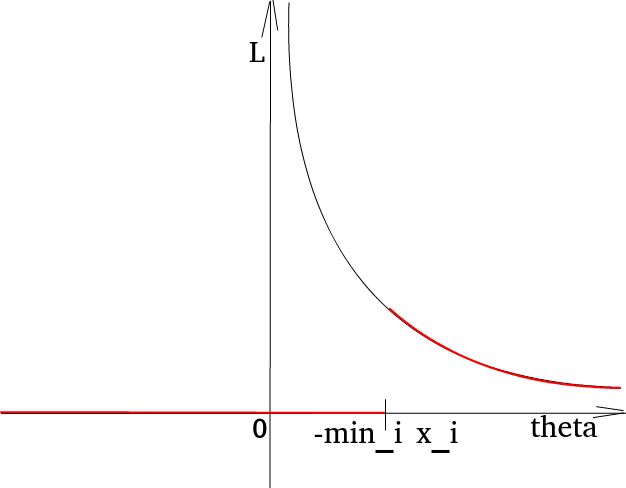
\includegraphics[width=.4\textwidth]{./pictures/4_18.png}
    \caption{График функции $L \left( \theta \right) $}
    \label{fig:418}
  \end{figure}

  Точка максимума этой функции --- это $ \left( - \min \limits_i x_i \right) $.

  Значит, $ \hat{ \theta } = - \min \limits_{1 \leq i \leq n} x_i$;
  \item плотность равномерного распределения на отрезке
  $ \left[- \theta, \theta \right], \, \theta > 0$ имеет вид
  $$p_{ \theta } \left( x \right) =
    \frac{ \mathbbm{1} \left\{ x \in \left[ - \theta, \theta \right] \right\} }{2 \theta }.$$

  По этой функции строим функцию правдоподобия
  $$L \left( \vec{x}, \theta \right) =
    \frac{ \mathbbm{1} \left\{ \vec{x} \in \left[ - \theta, \theta \right]^n \right\} }{ \left( 2 \theta \right)^n} =
    \frac{ \mathbbm{1} \left\{ \min \limits_i x_i \geq - \theta, \, \max \limits_i x_i \leq \theta \right\} }{ \left( 2 \theta \right)^n}.$$
  Меняем знак для минимального элемента выборки
  $$ \frac{ \mathbbm{1} \left\{ \min \limits_i x_i \geq - \theta, \, \max \limits_i x_i \leq \theta \right\} }{ \left( 2 \theta \right)^n} =
    \frac{1}{ \left( 2 \theta \right)^n} \cdot
    \mathbbm{1} \left\{
      \max \limits_i x_i \leq \theta, \, - \min \limits_i x_i \leq \theta
    \right\}.$$
  Берём максимум
  \begin{equation*}
    \begin{split}
      \frac{1}{ \left( 2 \theta \right)^n} \cdot
      \mathbbm{1} \left\{
        \max \limits_i x_i \leq \theta, \, - \min \limits_i x_i \leq \theta
      \right\} = \\
      = \frac{1}{ \left( 2 \theta \right)^n} \cdot
      \mathbbm{1} \left\{
        \max \left( \max \limits_i x_i, \, - \min \limits_i x_i \right) \leq \theta
      \right\}.
    \end{split}
  \end{equation*}

  Нарисуем график этой функции, как функции от $ \theta $ (рис. \ref{fig:4181}).

  \begin{figure}[h!]
    \centering
    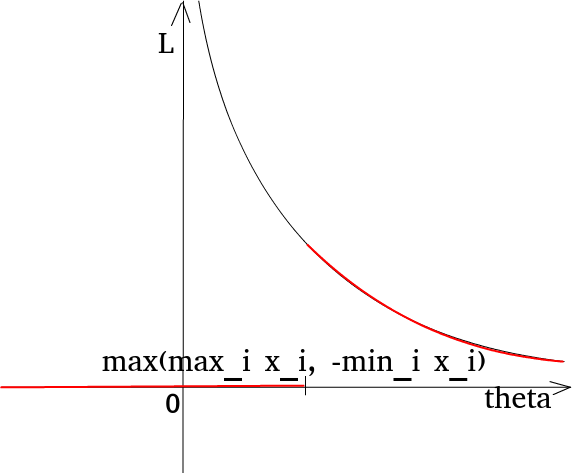
\includegraphics[width=.4\textwidth]{./pictures/4_18_1.png}
    \caption{График функции $L \left( \theta \right) $}
    \label{fig:4181}
  \end{figure}

  Точка максимума такой функции ---
  это $ \max \left( \max \limits_i x_i, \, - \min \limits_i x_i \right) $.

  Значит,
  $ \hat{ \theta } =
    \max \left(
      \max \limits_{1 \leq i\leq n} x_i, \, - \min \limits_{1 \leq i \leq n} x_i
    \right) $;
  \item плотность равномерного распределения на отрезке
  $ \left[ \theta , \theta + 2 \right], \, \theta \in \mathbb{R}$ имеет вид
  $$p_{ \theta } \left( x \right) =
    \frac{ \mathbbm{1} \left\{ x \in \left[ \theta, \theta + 2 \right] \right\} }{2}.$$

  По этой плотности строим функцию правдоподобия
  $$L \left( \vec{x}, \theta \right) =
    \frac{ \mathbbm{1} \left\{ \vec{x} \in \left[ \theta, \theta + 2 \right]^n \right\} }{2^n} =
    \frac{ \mathbbm{1} \left\{ \min \limits_i x_i \geq \theta, \, \max \limits_i x_i \leq \theta + 2 \right\} }{2^n}.$$
  Переносим 2 влево и именяем знак
  $$ \frac{ \mathbbm{1} \left\{ \min \limits_i x_i \geq \theta, \, \max \limits_i x_i \leq \theta + 2 \right\} }{2^n} =
    \frac{ \mathbbm{1} \left\{ \min \limits_i x_i \geq \theta, \, - \max \limits_i x_i + 2 \geq \theta \right\} }{2^n}.$$
  Берём максимум
  \begin{equation*}
    \begin{split}
      \frac{ \mathbbm{1} \left\{ \min \limits_i x_i \geq \theta, \, - \max \limits_i x_i + 2 \geq \theta \right\} }{2^n} = \\
      = \frac{ \mathbbm{1} \left\{ \max \left( \min \limits_i x_i,\, - \max \limits_i x_i + 2 \right) \geq \theta \right\} }{2^n}.
    \end{split}
  \end{equation*}

  Нарисуем график полученной функции, как функции от $ \theta $ (рис. \ref{fig:4182}).

  \begin{figure}[h!]
    \centering
    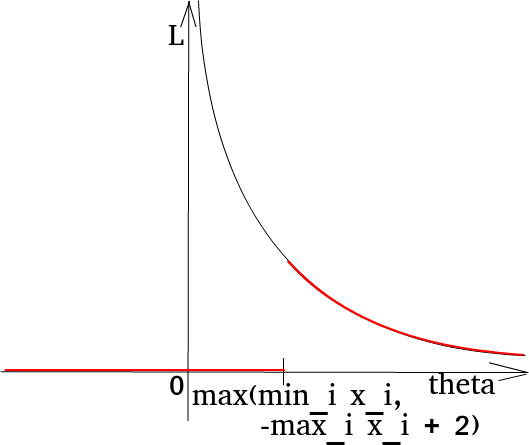
\includegraphics[width=.4\textwidth]{./pictures/4_18_2.png}
    \caption{График функции $L \left( \theta \right) $}
    \label{fig:4182}
  \end{figure}

  Точка максимума этой функции ---
  это $ \max \left( \min \limits_i x_i,\, - \max \limits_i x_i + 2 \right) $.

  Значит,
  $ \hat{ \theta } =
    \max \left(
      \min \limits_{1 \leq i \leq n} x_i,\, - \max \limits_{1 \leq i \leq n} x_i + 2
    \right) $;
  \item плотность равномерного распределения на отрезке
  $ \left[ \theta, 2 \theta \right], \, \theta > 0$ имеет вид
  $$p_{ \theta } \left( x \right) =
    \frac{ \mathbbm{1} \left\{ x \in \left[ \theta, 2 \theta \right] \right\} }{ \theta }.$$

  По этой функции строим функцию правдоподобия
  $$L \left( \vec{x}, \theta \right) =
    \frac{ \mathbbm{1} \left\{ \vec{x} \in \left[ \theta, 2 \theta \right]^n \right\} }{ \theta^n} =
    \frac{ \mathbbm{1} \left\{ \min \limits_i x_i \geq \theta, \, \max \limits_i x_i \leq 2 \theta \right\} }{ \theta^n}.$$
  Делим неравенство с максимумом на 2
  $$ \frac{ \mathbbm{1} \left\{ \min \limits_i x_i \geq \theta, \, \max \limits_i x_i \leq 2 \theta \right\} }{ \theta^n} =
    \frac{ \mathbbm{1} \left\{ \min \limits_i x_i \geq \theta,\, \frac{ \max \limits_i x_i}{2} \leq \theta \right\} }{ \theta^n}.$$
  Остюда следует, что
  $$ \frac{ \max \limits_i x_i}{2} \leq
    \theta \leq
    \min \limits_i x_i.$$

  Нарисуем график полученной функции, как функции от $ \theta $ (рис. \ref{fig:4183}).

  \begin{figure}[h!]
    \centering
    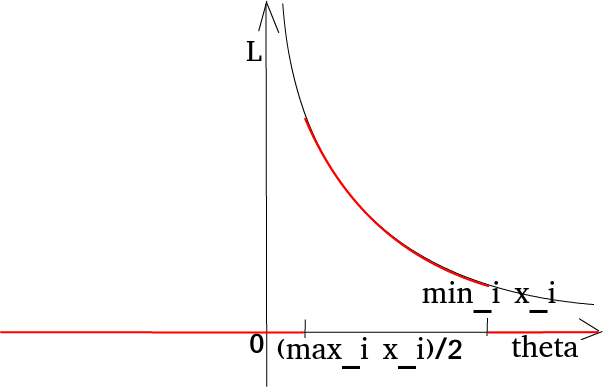
\includegraphics[width=.4\textwidth]{./pictures/4_18_3.png}
    \caption{График функции $L \left( \theta \right) $}
    \label{fig:4183}
  \end{figure}

  Точка максимума такой функции --- это
  $$ \frac{ \max \limits_i x_i}{2}.$$

  Значит,
  $$ \hat{ \theta } =
    \frac{ \max \limits_{1 \leq i \leq n} x_i}{2}.$$
\end{enumerate}

\subsubsection*{4.19}

\textit{Задание.}
Пусть $X_1, \dotsc, X_n$ ---
выборка из друхпараметрического показательного распределения с плотностью
$$f_{ \alpha, \beta } \left( y \right) =
  \begin{cases}
    \alpha^{-1} e^{- \frac{y - \beta }{ \alpha }}, \qquad y \geq \beta, \\
    0, \qquad otherwise,
  \end{cases}$$
где $ \alpha > 0, \, \beta \in \mathbb{R}$.
Постройте оценку максимального правдоподобия двумерного параметра $ \left( \alpha, \beta \right) $.
Проверьте состоятельность этой оценки.

\textit{Решение.}
Сейчас $ \theta $ будет векторным параметром, состоящим из двух элементов: $ \alpha, \beta $.

Плотность имеет вид
$$f_{ \alpha, \beta } \left( y \right) =
  \frac{1}{ \alpha } \cdot
  e^{- \frac{y}{ \alpha } + \frac{ \beta }{ \alpha }} \cdot
  \mathbbm{1} \left\{ y \geq \beta \right\}.$$

Произведение этих плотностей даёт
$$L \left( \vec{X}, \alpha, \beta \right) =
  \frac{1}{ \alpha^n} \cdot
  e^{- \frac{1}{ \alpha } \sum \limits_{i = 1}^n \left( X_i - \beta \right) } \cdot
  \mathbbm{1} \left\{ \vec{X} \in \left[ \beta, + \infty \right)^n \right\}.$$
Все элементы выборки не меньше, чем $ \beta $.
Запишем это условие через минимальный элемент
$$ \frac{1}{ \alpha^n} \cdot
  e^{- \frac{1}{ \alpha } \sum \limits_{i = 1}^n \left( X_i - \beta \right) } \cdot
  \mathbbm{1} \left\{ \vec{X} \in \left[ \beta, + \infty \right)^n \right\} =
  \frac{1}{ \alpha^n} \cdot
  e^{- \frac{1}{ \alpha } \sum \limits_{i = 1}^n \left( X_i - \beta \right) }
  \cdot \mathbbm{1} \left\{ \min \limits_{1 \leq i \leq n} X_i \geq \beta \right\}.$$

Найдём $ \beta^*$.
При фиксированном $ \alpha $ нарисуем график функции правдоподобия как функции от $ \beta $
(рис. \ref{fig:419}).

\begin{figure}[h!]
  \centering
  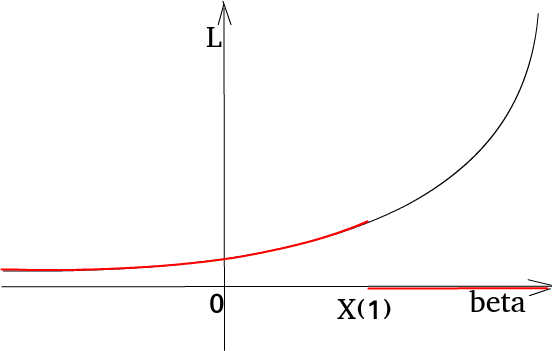
\includegraphics[width=.4\textwidth]{./pictures/4_19.png}
  \caption{График функции $L \left( \beta \right) $}
  \label{fig:419}
\end{figure}

Из графика видно, что точка максимума этой функции ---
это точка $ \min \limits_{1 \leq i \leq n} X_i = \beta^*$.

Так как есть экспонента, удобнее взять логарифм от функции правдоподобия
$$ln \left( \vec{X}, \alpha, \beta \right) =
  l \left( \vec{X}, \alpha, \beta \right) =
  -n ln \alpha + \frac{n \beta - \sum \limits_{i = 1}^n X_i}{ \alpha }.$$

Возьмём производную по $ \alpha $ и приравняем её к нулю
$$ \frac{ \partial l}{ \partial \alpha } =
  -n \cdot \frac{1}{ \alpha } - \frac{n \beta - \sum \limits_{i = 1}^n X_i}{ \alpha^2} =
  0.$$
Умножим на $ \left( - \alpha^2 \right) $ левую и правую части уравнения
$$n \alpha + n \beta - \sum \limits_{i = 1}^n X_i =
  0.$$

Отсюда выражаем оценку
$$ \alpha^* =
  \frac{1}{n} \sum \limits_{i = 1}^n X_i - \beta^* =
  \overline{X} - \min \limits_{1 \leq i \leq n} X_i.$$

Проверим состоятельность.
Нужно проверить,
выполняется ли
$$ \left( \alpha^*, \beta^* \right) \overset{P}{ \to } \left( \alpha , \beta \right), \,
  n \to \infty.$$

По определению
$P \left( \left| \beta^* - \beta \right| > \varepsilon \right) \to 0, \,
  n \to \infty, \,
  \forall \varepsilon > 0$.

Подставим в вероятность оценку
$$P \left( \left| \beta^* - \beta \right| > \varepsilon \right) =
  P \left( \left| \min \limits_{1 \leq i \leq n} X_i - \beta \right| > \varepsilon \right).$$

Из распределения $ \min \limits_{1 \leq i \leq n} X_i \geq \beta $, следовательно,
можем убрать модуль
$P \left( \left| \min \limits_{1 \leq i \leq n} X_i - \beta \right| > \varepsilon \right) =
  P \left( \min \limits_{1 \leq i \leq n} X_i - \beta > \varepsilon \right) =
  P \left( \min \limits_{1 \leq i \leq n} X_i > \beta + \varepsilon \right) = \\
  = P \left( \bigcap \limits_{i = 1}^n \left\{ X_i > \beta + \varepsilon \right\} \right) $.
Случайные величины независимые и одинаково распределённые
$P \left( \bigcap \limits_{i = 1}^n \left\{ X_i > \beta + \varepsilon \right\} \right) =
  \left[ P \left( X_1 > \beta + \varepsilon \right) \right]^n \to 0, \,
  n \to \infty,$
так как $P \left( X_1 > \beta + \varepsilon \right) \neq 1$.

Значит, $ \beta^*$ --- состоятельная оценка.
Тогда по закону больших чисел
$$ \alpha^* =
  \frac{1}{n} \sum \limits_{i = 1}^n X_i - \beta^* \overset{P}{ \to }
  MX_1 - \beta =
  \int \limits_{ \beta }^{+ \infty }
    \frac{1}{ \alpha } \cdot e^{- \frac{-y}{ \alpha }} e^{ \frac{ \beta }{ \alpha }} ydy -
  \beta. $$
Возьмём интеграл по частям
$$u = y, \,
  du = dy, \,
  dv = e^{- \frac{y}{ \alpha }} dy, \,
  v = \int e^{- \frac{y}{ \alpha }} dy = - \alpha e^{- \frac{y}{ \alpha }}.$$
Получим
$$ \int \limits_{ \beta }^{+ \infty }
    \frac{1}{ \alpha } \cdot e^{- \frac{-y}{ \alpha }} e^{ \frac{ \beta }{ \alpha }} ydy -
  \beta =
  \left.
    \frac{1}{ \alpha } \cdot
    e^{ \frac{ \beta }{ \alpha }} \left( - \alpha \right) y e^{- \frac{y}{ \alpha }}
  \right|_{ \beta }^{+ \infty } +
  \frac{1}{ \alpha } \cdot e^{ \frac{ \beta }{ \alpha }} \cdot \alpha \cdot
  \int \limits_{ \beta }^{+ \infty } e^{- \frac{y}{ \alpha }} dy -
  \beta.$$
Подставим пределы интегрирования и возьмём интеграл
$$ \left.
    \frac{1}{ \alpha } \cdot
    e^{ \frac{ \beta }{ \alpha }} \left( - \alpha \right) y e^{- \frac{y}{ \alpha }}
  \right|_{ \beta }^{+ \infty } +
  \frac{1}{ \alpha } \cdot e^{ \frac{ \beta }{ \alpha }} \cdot \alpha \cdot
  \int \limits_{ \beta }^{+ \infty } e^{- \frac{y}{ \alpha }} dy -
  \beta =
  e^{ \frac{ \beta }{ \alpha }} \beta \cdot e^{- \frac{ \beta }{ \alpha }} -
  e^{ \frac{ \beta }{ \alpha }} \cdot
  \left. \alpha e^{- \frac{y}{ \alpha }} \right|_{ \beta }^{+ \infty } -
  \beta.$$
Сократим экспоненты и подставим пределы интегрирования во втором слагаемом
$$e^{ \frac{ \beta }{ \alpha }} \beta \cdot e^{- \frac{ \beta }{ \alpha }} -
  e^{ \frac{ \beta }{ \alpha }} \cdot
  \left. \alpha e^{- \frac{y}{ \alpha }} \right|_{ \beta }^{+ \infty } -
  \beta =
  \beta + \alpha e^{ \frac{ \beta }{ \alpha }} \cdot e^{- \frac{ \beta }{ \alpha }} - \beta =
  \alpha.$$

Получили, что оценка $ \alpha^*$ --- тоже состоятельная.

\addcontentsline{toc}{chapter}{Занятие 5. Достаточные статистики}
\chapter*{Занятие 5. Достаточные статистики}

\addcontentsline{toc}{section}{Контрольные вопросы и задания}
\section*{Контрольные вопросы и задания}

\subsubsection*{Приведите определение условного распределения, определение достаточной статистики.}

$P \left( \xi \in \Delta \; \middle| \; \mathcal{F'} \right) =
  M \left[ \mathbbm{1}_{ \Delta } \left( \xi \right) \; \middle| \; \mathcal{F'} \right] $.

Статистика $T$ называется достаточной для параметра $ \theta $,
если условное распределение при известном $T$ не зависит от параметра $ \theta $.

\subsubsection*{Сформулируйте теорему про характеризацию достаточной статистики.}

Пусть $x_1, \dotsc, x_n$ ---
выборка из распределения с плотностью
$$p \left( x, \theta \right), \,
  \theta \in \Theta.$$

Статистика $T$ является достаточной тогда и только тогда,
когда функция правдоподобия $L \left( \vec{x}, \theta \right) $ допускает факторизацию,
то есть может быть представлена произведением двух функций следующего вида
$$L \left( \vec{x}, \theta \right) =
  h \left( T, \theta \right) \cdot g \left( \vec{x} \right).$$

\addcontentsline{toc}{section}{Аудиторные задачи}
\section*{Аудиторные задачи}

\subsubsection{5.3}

\textit{Задание.} Пусть $X_1, \dotsc, X_n$ --- выборка из распределения Бернулли с параметром $p$.
Выясните, является ли $ \overline{X}$ достаточной статистикой для параметра $p$.

\textit{Решение.} Записываем условное распределение.

Пусть $k_i = 0$ или $1$.

По определению условной вероятности
\begin{equation*}
  \begin{split}
    P \left\{ \left. X_1 = k_1, X_2 = k_2, \dotsc, X_n = k_n \right| \overline{X} = y \right\} = \\
    = \frac{P \left\{ X_1 = k_1, X_2 = k_2, \dotsc, X_n = k_n, \overline{X} = y \right\} }{P \left\{ \overline{X} = y \right\} }.
  \end{split}
\end{equation*}
Выборочное среднее $ \overline{X}$ выражаем через сумму
\begin{equation*}
  \begin{split}
    \frac{P \left\{ X_1 = k_1, X_2 = k_2, \dotsc, X_n = k_n, \overline{X} = y \right\} }{P \left\{ \overline{X} = y \right\} } = \\
    = \frac{P \left\{ X_1 = k_1, X_2 = k_2, \dotsc, X_n = k_n, \sum \limits_{i = 1}^n X_i = ny \right\} }{P \left\{ \sum \limits_{i = 1}^n X_i = ny \right\} }.
  \end{split}
\end{equation*}
Все $X_i$ --- независимы, следовательно, будет произведение вероятностей событий
\begin{equation*}
  \begin{split}
    \frac{P \left\{ X_1 = k_1, X_2 = k_2, \dotsc, X_n = k_n, \sum \limits_{i = 1}^n X_i = ny \right\} }{P \left\{ \sum \limits_{i = 1}^n X_i = ny \right\} } = \\
    = \frac{ \mathbbm{1} \left\{ \sum \limits_{i = 1}^n k_i = ny \right\} P \left\{ X_1 = k_1 \right\} \cdot \dotsc \cdot P \left\{ X_n = k_n \right\} }{P \left\{ \sum \limits_{i = 1}^n X_i = ny \right\} }.
  \end{split}
\end{equation*}
Сумма распределена по биномиальному распределению с параметрами $n, p$.
Подставляем значения вероятностей
\begin{equation*}
  \begin{split}
    \frac{ \mathbbm{1} \left\{ \sum \limits_{i = 1}^n k_i = ny \right\} P \left\{ X_1 = k_1 \right\} \cdot \dotsc \cdot P \left\{ X_n = k_n \right\} }{P \left\{ \sum \limits_{i = 1}^n X_i = ny \right\} } = \\
    = \frac{ \mathbbm{1} \left\{ \sum \limits_{i = 1}^n k_i = ny \right\} p^{k_1} \left( 1 - p \right)^{1 - k_1} \cdot \dotsc \cdot p^{k_n} \left( 1 - p \right)^{1 - k_n}}{C_n^{ny} p^{ny} \left( 1 - p \right)^{n + ny}}.
  \end{split}
\end{equation*}
Воспользуемся индикатором
\begin{equation*}
  \begin{split}
    \frac{ \mathbbm{1} \left\{ \sum \limits_{i = 1}^n k_i = ny \right\} \cdot p^{k_1} \left( 1 - p \right)^{1 - k_1} \cdot \dotsc \cdot p^{k_n} \left( 1 - p \right)^{1 - k_n}}{C_n^{ny} p^{ny} \left( 1 - p \right)^{n + ny}} = \\
    = \frac{ \mathbbm{1} \left\{ \sum \limits_{i = 1}^n k_i = ny \right\} \cdot p^{ny} \left( 1 - p \right)^{n - ny}}{C_n^{ny} p^{ny} \left( 1 - p \right)^{n - ny}}.
  \end{split}
\end{equation*}
Всё, что связано с $p$, пропадает
$$ \frac{ \mathbbm{1} \left\{ \sum \limits_{i = 1}^n k_i = ny \right\} \cdot p^{ny} \left( 1 - p \right)^{n - ny}}{C_n^{ny} p^{ny} \left( 1 - p \right)^{n - ny}} =
  \frac{ \mathbbm{1} \left\{ \sum \limits_{i = 1}^n k_i = ny \right\} }{C_n^{ny}}.$$

Зависимости от $p$ нет.
Отсюда следует, что $ \overline{X}$ --- достаточная статистика.

\subsubsection{5.4}

\textit{Задание.}
Пусть $X_1, \dotsc, X_n$ --- выборка из распределения Пуассона с параметром $ \lambda $.
Найдите условное распределение выборки при условии
$$X_1 + \dotsc + X_n = k.$$
Выясните, является ли $ \overline{X}$ достаточной статистикой для параметра $ \lambda $.

\textit{Решение.} Это дискретное распределение
\begin{equation*}
  \begin{split}
    P \left\{ X_1 = k_1, \dotsc, X_n = k_n \; \middle| \; \sum \limits_{i = 1}^n X_i = k \right\} = \\
    \frac{P \left\{ X_1 = k_1, \dotsc, X_n = k_n, \sum \limits_{i = 1}^n X_i = k \right\} }{P \left\{ \sum \limits_{i = 1}^n X_i = k \right\} }.
  \end{split}
\end{equation*}
Случайные величины $X_i$ --- независимы
\begin{equation*}
  \begin{split}
    \frac{P \left\{ X_1 = k_1, \dotsc, X_n = k_n, \sum \limits_{i = 1}^n X_i = k \right\} }{P \left\{ \sum \limits_{i = 1}^n X_i = k \right\} } = \\
    \frac{ \mathbbm{1} \left\{ \sum \limits_{i = 1}^n k_i = k \right\} P \left\{ X_1 = k_1 \right\} \cdot \dotsc \cdot P \left\{ X_n = k_n \right\} }{P \left\{ \sum \limits_{i = 1}^n X_i = k \right\} }.
  \end{split}
\end{equation*}
Имеем распределение Пуассона.
Сумма независимых случайных величин имеет распределение Пуассона с параметром $ \lambda n$.
Подставляем значения вероятностей
\begin{equation*}
  \begin{split}
    \frac{ \mathbbm{1} \left\{ \sum \limits_{i = 1}^n k_i = k \right\} P \left\{ X_1 = k_1 \right\} \cdot \dotsc \cdot P \left\{ X_n = k_n \right\} }{P \left\{ \sum \limits_{i = 1}^n X_i = k \right\} } = \\
    = \mathbbm{1} \left\{ \sum \limits_{i = 1}^n k_i = k \right\} \cdot
    \frac{ \frac{ \lambda^{k_1}}{k_1!} \cdot e^{- \lambda } \cdot \dotsc \cdot \frac{ \lambda^{k_n}}{k_n!} \cdot e^{- \lambda }}{ \frac{ \left( \lambda n \right)^k}{k!} \cdot e^{- \lambda }} =
    \frac{ \mathbbm{1} \left\{ \sum \limits_{i = 1}^n k_i = k \right\} k!}{k_1! \dotsc k_n! n^k}.
  \end{split}
\end{equation*}

Видим, что нет зависимости от $ \lambda $, следовательно, выборочное среднее $ \overline{X}$ ---
достаточная статистика для неизвестного $ \lambda $.

\subsubsection{5.5}

\textit{Задание.}
Пусть $X_1, \dotsc X_n$ ---
выборка из нормального распределение со средним $a$ и единичной дисперсией.
Найдите условное совместное распределение выборки при условии $X_1 + \dotsc + X_n = y$.
Выясните, является ли $ \overline{X}$ достаточной статистикой для параметра $a$.

\textit{Решение.} Нужно записать функцию правдоподобия
$$L \left( X_1, \dotsc, X_n, a \right) =
  \prod \limits_{i = 1}^n \frac{1}{ \sqrt{2 \pi }} \cdot e^{ \frac{- \left( X_i - a \right)^2}{2}} =
  \frac{1}{ \left( \sqrt{2 \pi } \right)^n} \cdot
  e^{- \sum \limits_{i = 1}^n \frac{ \left( X_i - a \right)^2}{2}}.$$
Откроем квадрат и запишем в статистических обозначениях
$$ \frac{1}{ \left( \sqrt{2 \pi } \right)^n} \cdot
  e^{- \sum \limits_{i = 1}^n \frac{ \left( X_i - a \right)^2}{2}} =
  \frac{1}{ \left( \sqrt{2 \pi } \right)^n} \cdot
  e^{- \frac{n \overline{X^2}}{2} an \overline{X} - \frac{a^2 n}{2}} =
  \frac{1}{ \left( \sqrt{2 \pi } \right)^n} \cdot e^{- \frac{n \overline{X^2}}{2}} \cdot
  e^{an \overline{X} - \frac{a^2 n}{2}},$$
где
$$ \frac{1}{ \left( \sqrt{2 \pi } \right)^n} \cdot e^{- \frac{n \overline{X^2}}{2}} =
  h \left( X_1, \dotsc, X_n \right), \,
  e^{an \overline{X} - \frac{a^2 n}{2}} = g \left( a, \overline{X} \right).$$

Предьявляем функции, о которых идёт речь в теореме.

По теореме про характеризацию достаточной статистики $ \overline{X}$ --- достаточная статистика.

\subsubsection{5.6}

\textit{Задание.}
Пусть $X_1, \dotsc, X_n$ ---
выборка из нормального распределения с нулевым средним и дисперсией $ \sigma^2$.
Найдите достаточную статистику со значениями в $ \mathbb{R}$ для параметра $ \sigma^2$.

\textit{Решение.}
$$L \left( \vec{X}, \sigma^2 \right) =
  \prod \limits_{i = 1}^n \frac{1}{ \sqrt{2 \pi } \sigma } \cdot e^{- \frac{X_i^2}{2 \sigma^2}} =
  \left( \frac{1}{ \sqrt{2 \pi } \sigma } \right)^n \cdot
  e^{- \frac{ \sum \limits_{i = 1}^n X_i^2}{2 \sigma^2}} =
  \frac{1}{ \left( \sqrt{2 \pi } \sigma \right)^n} \cdot
  e^{- \frac{n \overline{X^2}}{2 \sigma^2}}.$$

Достаточной статистикой будет второй выборочный момент.

$h \left( X_1, \dotsc, X_n \right) = 1$, тогда
$$g \left( \sigma^2, \overline{X^2} \right) =
  \frac{1}{ \left( \sqrt{2 \pi } \sigma \right)^n} \cdot
  e^{- \frac{n \overline{X^2}}{2 \sigma^2}}.$$

Для $ \sigma^2$ достаточная статистика --- $ \hat{ \sigma^2} = \overline{X^2}$.

\subsubsection{5.7}

\textit{Задание.}
Пусть $X_1, \dotsc, X_n$ ---
выборка из равномерного распределения на отрезке $ \left[ 0, \theta \right] $.
Найдите достаточную статистику со значениями в $ \mathbb{R}$ для параметра $ \theta $.

\textit{Решение.}
$$L \left( \vec{X}, \theta \right) =
  \prod \limits_{i = 1}^n
    \frac{1}{ \theta } \cdot \mathbbm{1} \left\{ X_i \in \left[ 0, \theta \right] \right\}.$$
Все $X_i$ должны быть не меньше нуля и не больше $ \theta $.
Получаем
$$ \prod \limits_{i = 1}^n
    \frac{1}{ \theta } \cdot \mathbbm{1} \left\{ X_i \in \left[ 0, \theta \right] \right\} =
  \frac{1}{ \theta^n} \cdot
  \mathbbm{1} \left\{ X_{ \left( 1 \right) } \geq 0, X_{ \left( n \right) } \leq \theta \right\}.$$
Разделим индекатор на 2
$$ \frac{1}{ \theta^n} \cdot
  \mathbbm{1} \left\{ X_{ \left( 1 \right) } \geq 0, X_{ \left( n \right) } \leq \theta \right\} =
  \mathbbm{1} \left\{ X_{ \left( 1 \right) } \geq 0 \right\} \cdot
  \frac{1}{ \theta^n} \cdot \mathbbm{1} \left\{ X_{ \left( n \right) } \leq \theta \right\},$$
где первый индикатор --- это функция $h \left( \vec{X} \right) $, всё остальное ---
$g \left( \theta, X_{ \left( n \right) } \right) $.

Вывод: $X_{ \left( n \right) }$ --- достаточная статистика для $ \theta $.

\subsubsection{5.8}

\textit{Задание.}
Пусть $X_1, \dotsc, X_n$ ---
выборка из равномерного распределения на отрезке $ \left[ a, b \right] $.
Выясните,
какие из статистик
$ \overline{X}, \,
  X_{ \left( n \right) }, \,
  \left( X_{ \left( 1 \right) }, X_{ \left( n \right) }) \right) $
являются достаточными для двумерного параметра $ \left( a, b \right) $.

\textit{Решение.} Для оценки $ \left( a, b \right) $ будет достаточно
$ \left( X_{ \left( 1 \right) }, X_{ \left( n \right) }) \right) $.

Информацию про средину отрезка даёт $ \overline{X}$.
Этой информации недостаточно для оценки концов .

Зная $X_{ \left( n \right) }$, будем знать, где правая граница, следовательно,
этой информации недостаточно.

Ищем функцию правдоподобия
$$L \left( \vec{X}, a, b \right) =
  \prod \limits_{i = 1}^n
    \frac{1}{b - a} \cdot \mathbbm{1} \left\{ X_i \in \left[ a, b \right] \right\} =
  \frac{1}{ \left( b - a \right)^n} \cdot
  \mathbbm{1} \left\{ X_{ \left( 1 \right) } \geq a, X_{ \left( n \right) } \leq b \right\}.$$
Записываем через функции, которые используются в теореме о характеризации достаточной статистики
$$ \frac{1}{ \left( b - a \right)^n} \cdot
  \mathbbm{1} \left\{ X_{ \left( 1 \right) } \geq a, X_{ \left( n \right) } \leq b \right\} =
  g \left( a, b, X_{ \left( 1 \right) }, X_{ \left( n \right) } \right), \,
  h \left( \vec{X} \right) = 1.$$
По теореме о характеризации, $ \left( X_{ \left( 1 \right) }, X_{ \left( n \right) } \right) $ ---
достаточная статистика для $ \left( a, b \right) $.

Допустим, $ \overline{X}$ --- достаточная статистика,
значит должно выполняться
$L \left( \vec{X}, a, b \right) =
  h \left( \vec{X} \right) \cdot g \left( a, b, \overline{X} \right) $.

Пусть имеем две выборки: $X_1^1, \dotsc, X_n^1$ и $X_1^2, \dotsc, X_n^2$,
причём
$$ \overline{X^1} =
  \overline{X^2} =
  c.$$

Допустим, что $X_{ \left( 1 \right) }^1 = a, \, X_{ \left( n \right) }^1 = b$, следовательно,
$X_i^1 \sim U \left( \left[ a, b \right] \right) $.

Вторую выборку подбираем так,
чтобы наблюдаемое значение выходило за пределы $ \left[ a, b \right] $, например,
$X_{ \left( 1 \right) }^2 < a$,
но $X_{ \left( i \right) }^2 \in \left( a, b \right) $ при $i \neq 1$.

Ищем функции правдоподобия для этих двух выборок
$$L \left( \vec{X^1} \right) =
  \frac{1}{ \left( b - a \right)^n} =
  h \left( \vec{X^1} \right) \cdot g \left( a, b, c \right), \,
  L \left( \vec{X^2} \right) =
  0 =
  h \left( \vec{X^2} \right) g \left( a, b, c \right).$$

Ноль --- реакция на индикатор.

Если бы взяли выборку внутри $ \left( a, b \right) $, то ничего бы не поменялось.

Но как только пересекаем границу, то есть реакция, то есть $h$ уже зависит от концов отрезка,
$h$ зависит от $a, b$.

Для статистики $X_{ \left( n \right) }$ --- аналогично.

\subsubsection{5.9}

\textit{Задание.}
Пусть $X_1, \dotsc, X_n$ ---
выборка из равномерного распределения на отрезке
$ \left[ a \left( \theta\ \right), b \left( \theta \right) \right] $.
Докажите,
что если $a \left( \theta \right) \uparrow, \, b \left( \theta \right) \downarrow $ с возрастанием
$ \theta $,
то статистика
$T =
  \min \left(
    a^{-1} \left( X_{ \left( 1 \right) } \right), b^{-1} \left( X_{ \left( n \right) } \right)
  \right) $
достаточная для параметра $ \theta $.

\textit{Решение.} Записываем функцию правдоподобия
$$L \left( \vec{X}, a \left( \theta \right), b \left( \theta \right) \right) =
  \prod \limits_{i = 1}^n
    \frac{1}{b \left( \theta \right) - a \left( \theta \right) } \cdot
    \mathbbm{1} \left\{
      X_i \in \left[ a \left( \theta \right), b \left( \theta \right) \right]
    \right\}.$$
Вычисляем произведение
\begin{equation*}
  \begin{split}
    \prod \limits_{i = 1}^n
      \frac{1}{b \left( \theta \right) - a \left( \theta \right) } \cdot
      \mathbbm{1} \left\{
        X_i \in \left[ a \left( \theta \right), b \left( \theta \right) \right]
      \right\} = \\
    = \frac{1}{ \left[ b \left( \theta \right) - a \left( \theta \right) \right]^n} \cdot
    \mathbbm{1} \left\{
      X_{ \left( 1 \right) } \geq a \left( \theta \right), \,
      X_{ \left( n \right) } \leq b \left( \theta \right)
    \right\}.
  \end{split}
\end{equation*}
Это строго монотонные функции.
Можем решить неравенства относительно $ \theta $.
Получим
\begin{equation*}
  \begin{split}
    \frac{1}{ \left[ b \left( \theta \right) - a \left( \theta \right) \right]^n} \cdot
    \mathbbm{1} \left\{
      X_{ \left( 1 \right) } \geq a \left( \theta \right), \,
      X_{ \left( n \right) } \leq b \left( \theta \right)
    \right\} = \\
    = \frac{1}{ \left[ b \left( \theta \right) - a \left( \theta \right) \right]^n} \cdot
    \mathbbm{1} \left\{
      \theta \leq a^{-1} \left( X_{ \left( 1 \right) } \right), \,
      \theta \leq b^{-1} \left( X_{ \left( n \right) } \right)
    \right\} = \\
    = \frac{1}{ \left[ b \left( \theta \right) - a \left( \theta \right) \right]^n} \cdot
    \mathbbm{1} \left\{ \theta \leq T \right\} =
    g \left( \theta, T \right),
  \end{split}
\end{equation*}
а $h \equiv 1$.

Отсюда $T$ --- достаточная статистика для $ \theta $.

\addcontentsline{toc}{section}{Домашнее задание}
\section*{Домашнее задание}

\subsubsection*{5.11}

\textit{Задание.}
Пусть $X_1, \dotsc, X_n$ --- выборка из биномиального распределения с параметрами $m$ и $p$.
Найдите условное распределение выборки при условии $X_1 + \dotsc, X_n = k$.
Выясните, является ли $ \overline{X}$ достаточной статистикой для параметра $p$ при известном $m$.

\textit{Решение.} Это дискретное распределение
\begin{equation*}
  \begin{split}
    P \left( X_1 = k_1, \dotsc, X_n = k_n \; \middle| \; \sum \limits_{i = 1}^n X_i = k \right) = \\
    = \frac{P \left( X_1 = k_1, \dotsc, X_n = k_n, \sum \limits_{i = 1}^n X_i = k \right) }{P \left( \sum \limits_{i = 1}^n X_i = k \right) }.
  \end{split}
\end{equation*}
Имеем биномиальное распределение.
Сумма независимых случайных величин имеет биномиальное распределение с параметрами $mn$ и $p$.
Подставляем значения вероятностей
\begin{equation*}
  \begin{split}
    \frac{P \left( X_1 = k_1, \dotsc, X_n = k_n, \sum \limits_{i = 1}^n X_i = k \right) }{P \left( \sum \limits_{i = 1}^n X_i = k \right) } = \\
    = \frac{ \mathbbm{1} \left\{ \sum \limits_{i = 1}^n k_i = k \right\} C_m^{k_1} p^{k_1} q^{m - k_1} \cdot \dotsc \cdot C_m^{k_n} p^{k_n} q^{m - k_n}}{C_{mn}^k p^k q^{mn-k}} = \\
    = \frac{ \mathbbm{1} \left\{ \sum \limits_{i = 1}^n k_i = k \right\} C_m^{k_1} \cdot \dotsc C_m^{k_n}}{C_{mn}^k}.
  \end{split}
\end{equation*}

Видим, что нет зависимости от $p$, следовательно, выборочное среднее $ \overline{X}$ ---
достаточная статистика для неизвестного $p$.

\subsubsection*{5.12}

\textit{Задание.}
Пусть $X_1, \dotsc, X_n$ ---
выборка из нормального распределения со средним $a$ и дисперсией $ \sigma^2$.
Найдите достаточную статистику со значениями в $ \mathbb{R}^2$ для двумерного параметра
$ \left( a, \sigma^2 \right) $.

\textit{Решение.} Ищем функцию правдоподобия
$$L \left( \vec{X}, a, \sigma^2 \right) =
  \prod \limits_{i = 1}^n
    \frac{1}{ \sqrt{2 \pi } \sigma } \cdot e^{- \frac{ \left( X_i - a \right)^2}{2 \sigma^2}} =
  \frac{1}{ \left( \sqrt{2 \pi } \sigma \right)^n} \cdot
  e^{- \frac{1}{2 \sigma^2} \sum \limits_{i = 1}^n \left( X_i - a \right)^2}.$$
Раскрываем квадрат
$$ \frac{1}{ \left( \sqrt{2 \pi } \sigma \right)^n} \cdot
  e^{- \frac{1}{2 \sigma^2} \sum \limits_{i = 1}^n \left( X_i - a \right)^2} =
  \frac{1}{ \left( \sqrt{2 \pi } \sigma \right)^n} \cdot
  e^{- \frac{1}{2 \sigma^2} \sum \limits_{i = 1}^n \left( X_i^2 - 2aX_i + a^2 \right) }.$$
Записываем через статистические величины
$$ \frac{1}{ \left( \sqrt{2 \pi } \sigma \right)^n} \cdot
  e^{- \frac{1}{2 \sigma^2} \sum \limits_{i = 1}^n \left( X_i^2 - 2aX_i + a^2 \right) } =
  \frac{1}{ \left( \sqrt{2 \pi } \sigma \right)^n} \cdot
  e^{- \frac{n \overline{X^2}}{2 \sigma^2}} \cdot e^{ \frac{n \overline{X} a}{2 \sigma^2}} \cdot
  e^{- \frac{a^2 n}{2 \sigma^2}}.$$
Эта величина равна
$g \left( a, \sigma^2, \overline{X}, \overline{X^2} \right), \,
  h \left( \vec{X} \right) = 1$.

По теореме о характеризации, $ \left( \overline{X}, \overline{X^2} \right) $ ---
достаточная статистика для $ \left( a, \sigma^2 \right) $.

\subsubsection*{5.13}

\textit{Задание.} Пусть $X_1, \dotsc, X_n$ --- выборка из равномерного распределения на отрезке
\begin{enumerate}[label=\alph*)]
  \item $ \left[ \theta, \theta + 1 \right] $;
  \item $ \left[ \theta, 2 \theta \right] $.
\end{enumerate}
Найдите достаточную для параметра $ \theta $ статистику со значениями в $ \mathbb{R}^2$.

\textit{Решение.}
\begin{enumerate}[label=\alph*)]
  \item Ищем функцию правдоподобия
  $$L \left( \vec{X}, \theta \right) =
    \prod \limits_{i = 1}^n
      \mathbbm{1} \left\{ X_i \in \left[ \theta, \theta + 1 \right] \right\}.$$
  Все $X_i$ должны быть не меньше $ \theta $ и не больше $ \left( \theta + 1 \right) $.
  Получаем
  $$ \prod \limits_{i = 1}^n
      \mathbbm{1} \left\{ X_i \in \left[ \theta, \theta + 1 \right] \right\} =
    \mathbbm{1} \left\{
      X_{ \left( 1 \right) } \geq \theta, X_{ \left( n \right) } \leq \theta + 1
    \right\}.$$
  Это равно $g \left( \theta, X_{ \left( 1 \right) }, X_{ \left( n \right) } - 1 \right), \,
    h \left( \vec{X} \right) = 1.$

  Вывод: $ \left( X_{ \left( 1 \right) }, X_{ \left( n \right) } - 1 \right) $ ---
  достаточная статистика для $ \theta $;
  \item ищем функцию правдоподобия
  $$L \left( \vec{X}, \theta \right) =
    \prod \limits_{i = 1}^n
      \frac{1}{ \theta } \cdot
      \mathbbm{1} \left\{ X_i \in \left[ \theta, 2 \theta \right] \right\}.$$
  Все $X_i$ должны быть не меньше чем $ \theta $, не больше $2 \theta $.
  Получим
  $$ \prod \limits_{i = 1}^n
      \frac{1}{ \theta } \cdot
      \mathbbm{1} \left\{ X_i \in \left[ \theta, 2 \theta \right] \right\} =
    \frac{1}{ \theta^n} \cdot
    \mathbbm{1} \left\{
      X_{ \left( 1 \right) } \geq \theta, X_{ \left( n \right) } \leq 2 \theta
    \right\}.$$
  Это равно
  $$g \left( \theta, X_{ \left( 1 \right) }, \frac{X_{ \left( n \right) }}{2} \right), \,
    h \left( \vec{X} \right) = 1.$$

  Вывод:
  $$ \left( X_{ \left( 1 \right) }, \frac{X_{ \left( n \right) }}{2} \right) $$
  --- достаточная статистика для $ \theta $.
\end{enumerate}

\subsubsection*{5.14}

\textit{Задание.}
Пусть $X_1, \dotsc, X_n$ ---
выборка из равномерного распределения на отрезке $ \left[ - \theta, \theta \right] $.
Найдите достаточную статистику для параметра $ \theta $ со значениями в $ \mathbb{R}$.

\textit{Решение.}
$$L \left( \vec{X}, \theta \right) =
  \prod \limits_{i = 1}^n
    \frac{1}{2 \theta } \cdot
    \mathbbm{1} \left\{ X_i \in \left[ - \theta, \theta \right] \right\}.$$
Все $X_i$ должны быть не меньше $ \left( - \theta \right) $ и не больше $ \theta $.
Получим
$$ \prod \limits_{i = 1}^n
    \frac{1}{2 \theta } \cdot
    \mathbbm{1} \left\{ X_i \in \left[ - \theta, \theta \right] \right\} =
  \frac{1}{ \left( 2 \theta \right)^n} \cdot
  \mathbbm{1} \left\{
    X_{ \left( 1 \right) } \geq - \theta, X_{ \left( n \right) } \leq \theta
  \right\}.$$
Умножим первое неравенство на $ \left( -1 \right) $.
Получим
\begin{equation*}
  \begin{split}
    \frac{1}{ \left( 2 \theta \right)^n} \cdot
    \mathbbm{1} \left\{
      X_{ \left( 1 \right) } \geq - \theta, X_{ \left( n \right) } \leq \theta
    \right\} = \\
    = \frac{1}{ \left( 2 \theta \right)^n} \cdot
    \mathbbm{1} \left\{
      - X_{ \left( 1 \right) } \leq \theta, X_{ \left( n \right) } \leq \theta
    \right\}.
  \end{split}
\end{equation*}
По теореме о характеризации это равно
$h \left( \vec{X} \right) \cdot
  g \left( \theta, \max \left( -X_{ \left( 1 \right) }, X_{ \left( n \right) } \right) \right).$

Вывод: $\max \left( -X_{ \left( 1 \right) }, X_{ \left( n \right) } \right) $ ---
достаточная статистика для $ \theta $.

\subsubsection*{5.16}

\textit{Задание.}
Пусть $X_1, \dotsc, X_n$ ---
выборка из равномерного распределения на отрезке
$ \left[ a \left( \theta \right), b \left( \theta \right) \right] $.
Докажите,
что если $a \left( \theta \right) \downarrow, \, b \left( \theta \right) \uparrow $
с возрастанием $ \theta $,
то статистика
$T =
  \max \left(
    a^{-1} \left( X_{ \left( 1 \right) } \right), b^{-1} \left( X_{ \left( n \right) } \right)
  \right) $
достаточная для параметра $ \theta $.
По выборке с равномерноым распределением на $ \left[ - \theta, \theta \right] $
найдите достаточную статистику для параметра $ \theta $ со значениями в $ \mathbb{R}$.

\textit{Решение.} Запишем функцию правдоподобия
$$L \left( \vec{X}, a \left( \theta \right), b \left( \theta \right) \right) =
  \prod \limits_{i = 1}^n
    \frac{1}{b \left( \theta \right) - a \left( \theta \right) } \cdot
    \mathbbm{1} \left\{
      X_i \in \left[ a \left( \theta \right), b \left( \theta \right) \right]
    \right\}.$$
Вычисляем произведение
\begin{equation*}
  \begin{split}
    \prod \limits_{i = 1}^n
      \frac{1}{b \left( \theta \right) - a \left( \theta \right) } \cdot
      \mathbbm{1} \left\{
        X_i \in \left[ a \left( \theta \right), b \left( \theta \right) \right]
      \right\} = \\
    = \frac{1}{ \left[ b \left( \theta \right) - a \left( \theta \right) \right]^n} \cdot
    \mathbbm{1} \left\{
      X_{ \left( 1 \right) } \geq a \left( \theta \right), \,
      X_{ \left( n \right) } \leq b \left( \theta \right)
    \right\}.
  \end{split}
\end{equation*}
Это строго монотонные функции.
Можем решить неравенства относительно $ \theta $.
Получим
\begin{equation*}
  \begin{split}
    \frac{1}{ \left[ b \left( \theta \right) - a \left( \theta \right) \right]^n} \cdot
  \mathbbm{1} \left\{
      X_{ \left( 1 \right) \geq a \left( \theta \right), \,
      X_{ \left( n \right) } \leq b \left( \theta \right) }
    \right\} = \\
    = \frac{1}{ \left[ b \left( \theta \right) - a \left( \theta \right) \right]^n} \cdot
    \mathbbm{1} \left\{
      \theta \geq a^{-1} \left( X_{ \left( 1 \right) } \right), \,
      \theta \geq b^{-1} \left( X_{ \left( n \right) } \right)
    \right\} = \\
    = \frac{1}{ \left[ b \left( \theta \right) - a \left( \theta \right) \right]^n} \cdot
    \mathbbm{1} \left\{ \theta \geq T \right\} =
    g \left( \theta, T \right),
  \end{split}
\end{equation*}
а $h \equiv 1$.

Значит, $T$ --- достаточная статистика для $ \theta $.

Для отрезка $ \left[ - \theta, \theta \right] $ получаем
$b \left( \theta \right) = \theta, \, a \left( \theta \right) = - \theta $.
Имеем неравенства $X_{ \left( 1 \right) } \geq - \theta, \, X_{ \left( n \right) } \leq \theta $,
откуда $ \theta \geq - X_{ \left( 1 \right) }, \, \theta \geq X_{ \left( n \right) }$, то есть
$$T =
  \max \left( -X_{ \left( 1 \right) }, X_{ \left( n \right) } \right).$$

\addcontentsline{toc}{chapter}{Занятие 6. Теорема Колмогорова про улучшение оценок.
                              Неравенство Рао-Крамера}
\chapter*{Занятие 6. Теорема Колмогорова про улучшение оценок. Неравенство Рао-Крамера}

\addcontentsline{toc}{section}{Контрольные вопросы и задания}
\section*{Контрольные вопросы и задания}

\subsubsection*{Приведите определение достаточной статистики.}

Статистика $T$ называется достаточной для параметра $ \theta $,
если условное распределение при известном $T$ не зависит от параметра $ \theta $.

\subsubsection*{Сформулируйте теорему про характеризацию достаточной статистики.}

Пусть $x_1, \dotsc, x_n$ ---
выборка из распределения с плотностью
$$p \left( x, \theta \right), \,
  \theta \in \Theta.$$

Статистика $T$ является достаточной тогда и только тогда,
когда функция правдоподобия $L \left( \vec{x}, \theta \right) $ допускает факторизацию,
то есть может быть представлена произведением двух функций следующего вида
$$L \left( \vec{x}, \theta \right) =
  h \left( T, \theta \right) \cdot g \left( \vec{x} \right).$$

\subsubsection*{Сформулируйте теорему Колмогорова про улучшение
                оценки с помощью достаточной статистики.}

Оптимальная оценка единственная (в том случае, когда она существует).

\subsubsection*{Что называется количеством информации Фишера?}

$$D_{ \theta } U \left( \vec{x}, \theta \right) =
  nD_{ \theta } \left(
    \frac{ \partial }{ \partial \theta } ln \, p \left( x, \theta \right)
  \right) =
  nI_0,$$
где $nI_0$ --- количество информации Фишера.

\subsubsection*{Запишите неравенство Рао-Крамера.}

Пусть $ \hat{ \theta }$ --- несмещённая оценка для параметра $ \theta $.
Тогда
$$ \forall \theta \in \Theta: \,
  D_{ \theta } \hat{ \theta } \geq \frac{1}{nI_0}.$$
Как угодно лучшую оценку взять нельзя.

\subsubsection*{Какая оценка называется эффективной?}

Если $ \hat{ \theta }$ такова, что $ \hat{ \theta }$ --- несмещённая и
$$D_{ \theta } \hat{ \theta } =
  \frac{1}{nI_0}, \,
  \theta \in \Theta,$$
то $ \hat{ \theta }$ называется эффективной оценкой.

\subsubsection*{Приведите определение экспоненциальной семьи распределений.}

\addcontentsline{toc}{section}{Аудиторные задачи}
\section*{Аудиторные задачи}

\subsubsection*{6.3}

\textit{Задание.}
Пусть $X_1, \dotsc, X_n$ ---
выборка из равномерного распределения на отрезке $ \left[ 0, \theta \right].$
Найдите несмещённую оценку неизвестного параметра
$ \tau \left( \theta, y \right) =
  P \left( X_1 > y \right) $
и улучшите её усреднением по достаточной для параметра $ \theta $ статистике.

\textit{Решение.} $X_{ \left( n \right) }$ --- достаточная статистика для $ \theta $.

Нужно найти $ \hat{ \tau }$ из условия, что она была бы несмещённой,
что
$$M \hat{ \tau } =
  \tau =
  P \left( X_1 > y \right).$$
Берём в качестве $ \hat{ \tau } = \mathbbm{1} \left\{ X_1 > y \right\} $ ---
это несмещённая оценка для $ \tau $.
Теперь улучшаем эту оценку.
$ \tau^* =
  M \left( \hat{ \tau } \; \middle| \; X_{ \left( n \right) } \right) =
  M \left\{ \mathbbm{1} \left\{ X_1 < y \right\} \; \middle| \; X_{ \left( n \right) } \right\}.$
Индикатор может принимать значения 0 и 1,
значит
\begin{equation*}
  \begin{split}
    M \left\{
      \mathbbm{1} \left\{ X_1 < y \right\} \; \middle| \; X_{ \left( n \right) }
    \right\} = \\
    = 0 \cdot
    P \left(
      \mathbbm{1} \left\{ X_1 > y \right\} = 0 \; \middle| \; X_{ \left( n \right) }
    \right) +
    1 \cdot
    P \left( \mathbbm{1} \left\{ X_1 > y \right\} = 1 \; \middle| \; X_{ \left( n \right) } \right).
  \end{split}
\end{equation*}
Первое слагаемое пропадает
\begin{equation*}
  \begin{split}
    0 \cdot
    P \left(
      \mathbbm{1} \left\{ X_1 > y \right\} = 0 \; \middle| \; X_{ \left( n \right) }
    \right) +
    1 \cdot
    P \left(
      \mathbbm{1} \left\{ X_1 > y \right\} = 1 \; \middle| \; X_{ \left( n \right) }
    \right) = \\
    = P \left( X_1 > y \; \middle| X_{ \left( n \right) } \right) =
    f \left( X_{ \left( n \right) } \right).
  \end{split}
\end{equation*}
Ищем $f \left( z \right) = P \left( X_1 > y \; \middle| \; X_{ \left( n \right) } = z \right).$
Выборка имеет равномерное распределение, то есть распределение, которое имеет плотность.
Вероятность попадания в точку равна нулю
$$ P \left( X_1 > y \; \middle| \; X_{ \left( n \right) } = z \right) =
  \lim \limits_{h \to 0}
    P \left\{ X_1 > y \; \middle| \; X_{ \left( n \right) } \in \left[ z, z + h \right] \right\}.$$
Воспользуемся определением условной вероятности
$$ \lim \limits_{h \to 0}
    P \left\{ X_1 > y \; \middle| \; X_{ \left( n \right) } \in \left[ z, z + h \right] \right\} =
  \lim \limits_{h \to 0}
    \frac{P \left\{ X_1 > y, X_{ \left( n \right) } \in \left[ z, z + h \right] \right\} }{P \left\{ X_{ \left( n \right) } \in \left[ z, z + h \right] \right\} }.$$
Это нужно рассматривать при $y < z$.
Разбиваем на разность двух вероятностей в числителе и знаменателе
\begin{equation*}
  \begin{split}
    \lim \limits_{h \to 0}
      \frac{P \left\{ X_1 > y, X_{ \left( n \right) } \in \left[ z, z + h \right] \right\} }{P \left\{ X_{ \left( n \right) } \in \left[ z, z + h \right] \right\} } = \\
    = \lim \limits_{h \to 0} \left[
      \frac{P \left\{ X_1 > y, X_{ \left( n \right) } \leq z + h \right\} }{P \left\{ X_{ \left( n \right) } \leq z + h \right\} - P \left\{ X_{ \left( n \right) } \leq z \right\} } -
      \frac{P \left\{ X_1 > y, X_{ \left( n \right) } \leq z \right\} }{P \left\{ X_{ \left( n \right) } \leq z + h \right\} - P \left\{ X_{ \left( n \right) } \leq z \right\} }
    \right].
  \end{split}
\end{equation*}
Переходим к функции распределения выборки
\begin{equation*}
  \begin{split}
    \lim \limits_{h \to 0} \left[
      \frac{P \left\{ X_1 > y, X_{ \left( n \right) } \leq z + h \right\} }{P \left\{ X_{ \left( n \right) } \leq z + h \right\} - P \left\{ X_{ \left( n \right) } \leq z \right\} } -
      \frac{P \left\{ X_1 > y, X_{ \left( n \right) } \leq z \right\} }{P \left\{ X_{ \left( n \right) } \leq z + h \right\} - P \left\{ X_{ \left( n \right) } \leq z \right\} }
    \right] = \\
    = \lim \limits_{h \to 0} \left\{
      \frac{ \left[ F \left( z + h \right) - F \left( y \right) \right] \left[ F \left( z + h \right) \right]^{n - 1}}{ \left[ F \left( z + h \right) \right]^n - \left[ F \left( z \right) \right]^n} -
      \frac{ \left[ F \left( z \right) - F \left( y \right) \right] \left[ F \left( z \right) \right]^{n - 1}}{ \left[ F \left( z + h \right) \right]^n - \left[ F \left( z \right) \right]^n}
    \right\}.
  \end{split}
\end{equation*}

Знаменатель и числитель стремятся к нулю.
Дифференцируем по $h$ числитель и знаменатель.
Это правило Лопиталя
\begin{equation*}
  \begin{split}
    \lim \limits_{h \to 0} \left\{
      \frac{ \left[ F \left( z + h \right) - F \left( y \right) \right] \left[ F \left( z + h \right) \right]^{n - 1}}{ \left[ F \left( z + h \right) \right]^n - \left[ F \left( z \right) \right]^n} -
      \frac{ \left[ F \left( z \right) - F \left( y \right) \right] \left[ F \left( z \right) \right]^{n - 1}}{ \left[ F \left( z + h \right) \right]^n - \left[ F \left( z \right) \right]^n}
    \right\} = \\
    = \lim \limits_{h \to 0} \left\{
      \frac{p \left( z + h \right) \left[ F \left( z + h \right) \right]^{n - 1}}{n \left[ F \left( z + h \right) \right]^{n - 1} p \left( z + h \right) } +
      \frac{ \left( n + 1 \right) \left[ F \left( z + h \right) \right]^{n - 2} p \left( z + h \right) \left[ F \left( z + h \right) - F \left( y \right) \right] }{n \left[ F \left( z + h \right) \right]^{n - 1} p \left( z + h \right) }
    \right\} = \\
    = \lim \limits_{h \to 0}
      \frac{F \left( z + h \right) + \left( n - 1 \right) \left[ F \left( z + h \right) - F \left( y \right) \right] }{nF \left( z + h \right) }.
  \end{split}
\end{equation*}
Переходим к пределу
$$ \lim \limits_{h \to 0}
    \frac{F \left( z + h \right) + \left( n - 1 \right) \left[ F \left( z + h \right) - F \left( y \right) \right] }{nF \left( z + h \right) } =
  \frac{F \left( z \right) + \left( n + 1 \right) \left[ F \left( z \right) - F \left( y \right) \right] }{nF \left( z \right) }.$$
Приводим подобные
$$ \frac{F \left( z \right) + \left( n + 1 \right) \left[ F \left( z \right) - F \left( y \right) \right] }{nF \left( z \right) } =
  \frac{nF \left( z \right) - \left( n - 1 \right) F \left( y \right) }{nF \left( z \right) }.$$
Почленно поделим числитель на знаменатель
$$ \frac{nF \left( z \right) - \left( n - 1 \right) F \left( y \right) }{nF \left( z \right) } =
  1 - \frac{n - 1}{n} \cdot \frac{F \left( y \right) }{F \left( z \right) }.$$
Подставляем значения функции равномерного распределения на отрезке $ \left[ 0, \theta \right] $.
Получаем
$$1 - \frac{n - 1}{n} \cdot \frac{F \left( y \right) }{F \left( z \right) } =
  1 - \frac{n - 1}{n} \cdot \frac{y}{z}.$$

Окончательно
$$f \left( X_{ \left( n \right) } \right) =
  1 - \frac{n - 1}{n} \cdot \frac{y}{X_{ \left( n \right) }}.$$

\subsubsection*{6.4}

\textit{Задание.}
Пусть $X_1, \dotsc, X_n$ --- выборка из распределения Пуассона с параметром $ \lambda $.
В качестве оценки параметра $ \theta = e^{- \lambda }$ рассматривают статистику
$ \hat{ \theta } =
  \mathbbm{1} \left\{ X_1 = 0 \right\} $.
Вычислите смещение $b_n \left( \theta \right) = M \hat{ \theta } - \theta $
этой оценки и улучшите её усреднением по достаточной статистике для параметра
$ \theta $ статистикой.

\textit{Решение.} Неизвестный параметр --- это $e^{- \lambda } = \theta $.

Ищем смещение
$M \hat{ \theta } =
  M \mathbbm{1} \left\{ X_1 = 0 \right\} =
  P \left\{ X_1 = 0 \right\} =
  e^{- \lambda } =
  \theta $,
значит, смещение $b_n \left( \theta \right) = 0$.
Это несмещённая оценка.

Займёмся поиском достаточной статистики
$$L \left( \vec{X}, \lambda \right) =
  \prod \limits_{i = 1}^n \frac{ \lambda^{X_i}}{X_i!} \cdot e^{- \lambda } =
  \frac{ \lambda^{n \overline{X}}}{X_1! \dotsc X_n!} \cdot e^{- \lambda n} =
  \frac{1}{X_1! \dotsc X_n!} \cdot \lambda^{n \overline{X}} e^{- \lambda n}.$$

Вывод: $ \overline{X}$ --- достаточная статистика для $ \lambda $, а значит и для $ \theta $,
как функции от $ \lambda $.

Нудно найти условное математическое ожидание
$M \left( \hat{ \theta } \; \middle| \; \overline{X} \right) =
  f \left( \overline{X} \right) $.
Начнём с
$f \left( y \right) =
  M \left( \hat{ \theta } \; \middle| \; \overline{X} = y \right) =
  M \left( \mathbbm{1} \left\{ X_1 = 0 \right\} \; \middle| \; \overline{X} = y \right) $.
Индикатор --- это дискретная случайная величина, которая принимает 2 значения
$$M \left( \mathbbm{1} \left\{ X_1 = 0 \right\} \; \middle| \; \overline{X} = y \right) =
  1 \cdot P \left( X_1 = 0 \; \middle| \; \overline{X} = y \right) =
  \frac{P \left( X_1 = 0, \sum \limits_{i = 1}^n X_i = ny \right) }{P \left( \sum \limits_{i = 1}^n X_i = ny \right) }.$$
В числителе стоит случайное событие $X_1 = 0$.
Оно означает, что суммировать можно от двух
$$ \frac{P \left( X_1 = 0, \sum \limits_{i = 1}^n X_i = ny \right) }{P \left( \sum \limits_{i = 1}^n X_i = ny \right) } =
  \frac{P \left( X_1 = 0 \right) P \left( \sum \limits_{i = 2}^n X_i = ny \right) }{P \left( \sum \limits_{i = 1}^n X_i = ny \right) }.$$
Сумма независимых пуассоновских случайных величин имеет распределение Пуассона с параметром,
который равен сумме параметров
$$ \frac{P \left( X_1 = 0 \right) P \left( \sum \limits_{i = 2}^n X_i = ny \right) }{P \left( \sum \limits_{i = 1}^n X_i = ny \right) } =
  \frac{e^{- \lambda } \cdot \frac{ \left( \left( n - 1 \right) \lambda \right)^{ny}}{ \left( ny \right)!} \cdot e^{- \lambda \left( n - 1 \right) }}{ \frac{ \left( n \lambda \right)^{ny}}{ \left( ny \right)!} \cdot e^{- \lambda n}} =
  \left( \frac{n - 1}{n} \right)^{ny}.$$

Чтобы записать ответ, нужно вместо $y$ записать $ \overline{X}$.
Получим
$$ \left( \frac{n - 1}{n} \right)^{n \overline{X}}.$$
Когда $n \to \infty $, эта оценка стремится к $e^{- \overline{X}}$.

\subsubsection*{6.5}

\textit{Задание.}
Пользуясь неравенством Рао-Крамера, выясните,
является ли эффективной оценка $ \overline{X}$ параметра $p$ распределения Бернулли.

\textit{Решение.} $X_1, \dotsc, X_n$ --- выборка.

Несмещённой оценкой для параметра является $ \hat{p} = \overline{X}$.
Формально в этом убедимся.
Итак,
$$M \hat{p} =
  M \overline{X} =
  \frac{1}{n} \cdot M \sum \limits_{i = 1}^n X_i.$$
Все случайные величины одинаково распределены, следовательно, все математические ожидания совпадают
$$ \frac{1}{n} \cdot M \sum \limits_{i = 1}^n X_i =
  \frac{1}{n} \cdot n MX_1 =
  MX_1 =
  p.$$

Ищем дисперсию
$$D \hat{p} =
  D \overline{X} =
  D \left( \frac{1}{n} \sum \limits_{i = 1}^n X_i \right) =
  \frac{1}{n^2} \cdot D \sum \limits_{i = 1}^n X_i.$$
Дисперсии равны.
Случайные величины независимы, следовательно, дисперсия суммы --- это сумма дисперсий
$$ \frac{1}{n^2} \cdot D \sum \limits_{i = 1}^n X_i =
  \frac{1}{n^2} \cdot nDX_1 =
  \frac{1}{n} \cdot p \left( 1 - p \right).$$

Сначала нужна функция правдоподобия для одного наблюдения
$$L \left( X_1, p \right) =
  p^{X_1} \left( 1 - p \right)^{1 - X_1}.$$
Логарифмируем
$ln \, L \left( X_1, p \right) =
  X_1 \, ln \, p + \left( 1 - p \right) ln \left( 1 - p \right) $.
Ищем первую производную
$$ \frac{ \partial }{ \partial p} ln \, L \left( X_1, p \right) =
  \frac{X_1}{p} - \frac{1 - X_1}{1 - p}.$$
Ищем вторую производную
$$ \frac{ \partial^2}{ \partial p^2} ln \, L \left( X_1, p \right) =
  - \frac{X_1}{p^2} - \frac{1 - X_1}{ \left( 1 -p \right)^2}.$$
Пишем количество информации.
Берём математическое ожидание со знаком <<минус>>
$$I \left( \theta \right) =
  M \left( \frac{X_1}{p} + \frac{1 - X_1}{ \left( 1 - p \right)^2} \right) =
  \frac{1}{p} + \frac{1 - p}{ \left( 1 - p \right)^2} =
  \frac{1}{p} + \frac{1}{1 - p}.$$
Приводим к общему знаменателю
$$ \frac{1}{p} + \frac{1}{1 - p} =
  \frac{1 - p + p}{p \left( 1 - p \right) } =
  \frac{1}{p \left( 1 - p \right) }.$$

Ищем обратную величину, делённую на $n$.
Получаем
$$ \frac{1}{nI \left( \theta \right) } =
  \frac{1}{n \left[ p \left( 1 - p \right) \right]^{-1}} =
  \frac{p \left( 1 - p \right) }{n} =
  D \hat{p},$$
следовательно, $ \hat{p}$ --- эффективная оценка параметра $p$.

\subsubsection*{6.6}

\textit{Задание.}
Пусть $X_1, \dotsc, X_n$ --- выборка из равномерного рпспределения с параметром $p$.
Выясните, является ли эффективной оценка $ \hat{ \theta } = 1 + \overline{X}$ параметра
$$ \theta =
  \frac{1}{p}.$$

\textit{Решение.} Берём дисперсию
$$D \hat{ \theta } =
  D \left( 1 + \overline{X} \right) =
  D \overline{X} =
  D \left( \frac{1}{n} \sum \limits_{i = 1}^n X_i \right) =
  \frac{1}{n^2} \cdot D \sum \limits_{i = 1}^n X_i =
  \frac{1}{n^2} \cdot nDX_1.$$
Сократим $n$ и подставим значение дисперсии равномерного распределения
$$ \frac{1}{n^2} \cdot nDX_1 =
  \frac{1}{n} \cdot \frac{1 - p}{p^2}.$$
Можем записать это как функцию от $ \theta $.
Получим
$$ \frac{1}{n} \cdot \frac{1 - p}{p^2} =
  \frac{1}{n} \cdot \left( \theta^2 - \theta \right).$$
Можно $ \theta $ вынести за скобки
$$ \frac{1}{n} \cdot \left( \theta^2 - \theta \right) =
  \frac{ \theta }{n} \cdot \left( \theta - 1 \right).$$
Записываем функцию правдоподобия для одного наблюдения
$$L \left( X_1, p \right) =
  p \left( 1 - p \right)^{X_1}.$$

Подставим оценку параметра
$$L \left( X_1, \theta \right) =
  \frac{1}{ \theta } \cdot \left( 1 - \frac{1}{ \theta } \right)^{X_1} =
  \frac{1}{ \theta^{X_1 + 1}} \cdot \left( \theta - 1 \right)^{X_1}.$$

Логарифмируем
$ln \, L \left( X_1, \theta \right) =
  - \left( X_1 + 1 \right) ln \, \theta + X_1 ln \left( \theta - 1 \right) $.
Берём первую производную
$$ \frac{ \partial }{ \partial \theta } ln \, L \left( X_1, \theta \right) =
  - \frac{X_1 + 1}{ \theta } + \frac{X_1}{ \theta - 1}.$$

Берём вторую производную
$$ \frac{ \partial^2}{ \partial \theta^2} ln \, L \left( X_1, \theta \right)  =
  \frac{X_1 + 1}{ \theta^2} - \frac{X_1}{ \left( \theta - 1 \right)^2}.$$
Берём математическое ожидание
$$MX_1 =
  \frac{1 - p}{p}.$$
Почленно поделим числитель на знаменатель
$$ \frac{1 - p}{p} =
  \theta - 1.$$

Берём математическое ожидание второй производной функции правдоподобия со знаком <<минус>>
$$-M \left[ \frac{ \partial^2}{ \partial \theta^2} ln \, L \left( X_1, \theta \right) \right] =
  - \frac{ \theta }{ \theta^2} + \frac{ \theta - 1}{ \left( \theta - 1 \right)^2} =
  - \frac{1}{ \theta } + \frac{1}{ \theta - 1} =
  \frac{- \theta + 1 + \theta }{ \theta \left( \theta - 1 \right) }.$$
Приводим подобные
$$ \frac{- \theta + 1 + \theta }{ \theta \left( \theta - 1 \right) } =
  \frac{1}{ \theta \left( \theta - 1 \right) } =
  I \left( \theta \right).$$

Формируем обратную величину и делим на $n$.
Значит,
$$ \frac{1}{nI \left( \theta \right) } =
  \frac{ \theta \left( \theta - 1 \right) }{n} =
  D \hat{ \theta }.$$
Получили, что оценка эффективная.

\subsubsection*{6.7}

\textit{Задание.}
Пусть $X_1, \dotsc, X_n$ ---
выборка из распределения $N \left( \theta, \sigma^2 \right) $ с неизвестным параметром $ \theta $
и известной дисперсией.
Выясните,
является ли статистика $ \theta^* = \overline{X}$ эффективной оценкой параметра $ \theta $.

\textit{Решение.} Проверим несмещённость
$$M \theta^* =
  M \overline{X} =
  M \left( \frac{1}{n} \sum \limits_{i = 1}^n X_i \right) =
  \frac{1}{n} \cdot M \sum \limits_{i = 1}^n X_1 =
  \frac{1}{n} \cdot nMX_1 =
  \theta.$$
Несмещённость есть.
Ищем дисперсию
$$D \theta^* =
  D \overline{X} =
  D \left( \frac{1}{n} \sum \limits_{i = 1}^n X_i \right) =
  \frac{1}{n^2} \cdot D \sum \limits_{i = 1}^n X_i.$$
Воспользуемся независимостью случайных величин в выборке
$$ \frac{1}{n^2} \cdot D \sum \limits_{i = 1}^n X_i -
  \frac{1}{n^2} \cdot nDX_1.$$
Случайные величины в выборке одинаково распределены, значит
$$ \frac{1}{n^2} \cdot nDX_1 =
  \frac{ \sigma^2}{n}.$$

Переходим к функции правдоподобия и оценке количества информации.
Смотрим на одно наблюдение
$$L \left( X_1, \theta \right) =
  \frac{1}{ \sqrt{2 \pi } \sigma } \cdot e^{- \frac{ \left( X_1 - \theta \right) }{2 \sigma^2}}.$$
Логарифмируем
$$ln \, L \left( X_1, \theta \right) =
  ln \left( \frac{1}{ \sqrt{2 \pi } \sigma } \right) -
  \left( X_1 - \theta \right)^2 \cdot \frac{1}{2 \sigma^2}.$$

Ищем первую производную
$$ \frac{ \partial }{ \partial \theta } ln \, L \left( X_1, \theta \right) =
  2 \left( X_1 - \theta \right) \cdot \frac{1}{2 \sigma^2} =
  \frac{X_1 - \theta }{ \sigma^2}.$$
Ищем вторую производную
$$ \frac{ \partial }{ \partial \theta^2} ln \, L \left( X_1, \theta \right) =
  - \frac{1}{ \sigma^2}.$$
Таким образом,
$$I \left( \theta \right) =
  -M \left( - \frac{1}{ \sigma^2} \right) =
  \frac{1}{ \sigma^2}.$$
Формируем величину
$$ \frac{1}{nI \left( \theta \right) } =
  \frac{ \sigma^2}{n} =
  D \theta^*,$$
значит, оценка эффективная.

\addcontentsline{toc}{section}{Домашнее задание}
\section*{Домашнее задание}

\subsubsection*{6.10}

\textit{Задание.}
Пусть $X_1, \dotsc, X_n$ ---
выборка из нормального распределения с параметрами $ \left( a, 1 \right) $.
Улучшите оценку $ \hat{a} = X_1$ усреднением по фиксированному значению достаточной
статистики $ \overline{X}$.
Найдите распределение, математическое ожидание и дисперсию улучшенной оценки.

\textit{Решение.} Улучшаем оценку
$$a^* =
  M \left( \hat{a} \; \middle| \; \overline{X} \right) =
  M \left( X_1 \; \middle| \; \overline{X} \right) =
  \frac{1}{n} \sum \limits_{i = 1}^n M \left( X_i \; \middle| \; \overline{X} \right) =
  M \left( \frac{1}{n} \sum \limits_{i = 1}^n X_i \; \middle| \; \overline{X} \right).$$
Запишем через выборочное среднее
$$M \left( \frac{1}{n} \sum \limits_{i = 1}^n X_i \; \middle| \; \overline{X} \right) =
  M \left( \overline{X} \; \middle| \; \overline{X} \right) =
  \overline{X}.$$

Математическое ожидание равно
$$Ma^* =
  M \overline{X} =
  M \left( \frac{1}{n} \sum \limits_{i = 1}^n X_i \right) =
  \frac{1}{n} \sum \limits_{i = 1}^n MX_i =
  \frac{1}{n} \cdot na =
  a,$$
дисперсия ---
$$Da^* =
  D \left( \frac{1}{n} \sum \limits_{i = 1}^n X_i \right) =
  \frac{1}{n^2} \cdot n DX_1 =
  \frac{1}{n} \cdot 1 =
  \frac{1}{n}.$$

Она имеет нормальное распределение
$$a^* \sim
  N \left( a, \frac{1}{n} \right).$$

Так как $Ma^* = a$, то оценка несмещённая.

\subsubsection*{6.11}

\textit{Задание.}
Пусть $X_1, \dotsc, X_n$ --- выборка из распределения Пуассона с параметром $ \lambda $.
В качестве оценки параметра $ \theta = e^{- \lambda }$ рассматривают статистику
$$ \hat{ \theta } =
  \overline{ \mathbbm{1} \left\{ X = 0 \right\} } =
  \frac{1}{n} \sum \limits_{i = 1}^n \mathbbm{1} \left\{ X_i = 0 \right\}.$$
Вычислите смещение $b_n \left( \theta \right) = M \hat{ \theta } - \theta $ этой оценки и выясните,
является ли она эффективной.

\textit{Решение.}
$$M \hat{ \theta } =
  M \left( \frac{1}{n} \sum \limits_{i = 1}^n \mathbbm{1} \left\{ X_i = 0 \right\} \right) =
  \frac{1}{n} M \left( \sum \limits_{i = 1}^n \mathbbm{1} \left\{ X_i = 0 \right\} \right) =
  \frac{1}{n} \cdot \sum \limits_{i = 1}^n P \left( X_i = 0 \right).$$
Подставляем значение вероятности для распределения Пуассона
$$ \frac{1}{n} \cdot \sum \limits_{i = 1}^n P \left( X_i = 0 \right) =
  \frac{1}{n} \cdot \sum \limits_{i = 1}^n \frac{ \lambda^0}{0!} \cdot e^{- \lambda } =
  \frac{1}{n} \cdot e^{- \lambda } \cdot n =
  e^{- \lambda }.$$

Подставляем полученное значение в формулу для смещения
$$b_n \left( \theta \right) =
  M \hat{ \theta } - \theta =
  e^{- \lambda } - e^{- \lambda } =
  0.$$

\addcontentsline{toc}{chapter}{Занятие 7. Гауссовые системы}
\chapter*{Занятие 7. Гауссовые системы}

\addcontentsline{toc}{section}{Контрольные вопросы и задания}
\section*{Контрольные вопросы и задания}

\subsubsection*{Приведите определение гауссового случайного вектора,
                ковариационной матрицы гауссового случаайного вектора.}

$ \vec{ \xi } = \left( \xi_1, \dotsc, \xi_n \right) $ --- гауссовый, если
$$ \forall \alpha_1, \dotsc, \alpha_n: \,
  \sum \limits_{k = 1}^n \alpha_k \xi_k$$
--- гауссовская случайная величина.

$A = cov_{ \vec{ \xi } \vec{ \xi }}, \,
  A_{ij} =
  cov \left( \xi_i, \xi_j \right) =
  M \left( \xi_i \xi_j \right) - M \xi_i M \xi_j$.

\subsubsection*{Какими свойствами владеет ковариационная матрица?}

$A_{ii} = D \xi_i \geq 0$ --- на диагонале --- неотрицательные числа.

Матрица симметрична: $A_{ij} = A_{ji}$.

Матрица неотрицательно определена.

\subsubsection*{Как изменяются характеристики гауссового случайного
                вектора при действии на него линейного оператора?}
Пускай $ \vec{ \xi }$ случайный $n$-элементный вектор,
имеющий гауссовское распределение с параметрами $ \vec{a}$ и
$A, \,
  \vec{ \xi } \sim N \left( \vec{a}, A \right), \,
  \vec{b} \in \mathbb{R}^m, \,
  T \in \mathbb{R}^{m \times n}$.
Тогда $T \vec{ \xi } + \vec{b} \sim N \left( T \vec{a} + \vec{b}, TAT^* \right) $.

\subsubsection*{При каких условиях гауссовский случайный вектор имеет плотность распределения?}

Плотность можно записать только в случае, когда $det \, A \neq 0$.

\subsubsection*{Запишите плотность распределения гауссового случайного вектора.}

$$p_{ \vec{ \xi }} \left( \vec{x} \right) =
  \left( \frac{1}{ \sqrt{2 \pi }} \right)^n \cdot \frac{1}{ \sqrt{det \, A}} \cdot
  e^{- \frac{1}{2} \left[ \vec{x} - \vec{a}, A^{-1} \left( \vec{x} - \vec{a} \right) \right] }.$$

\subsubsection*{Сформулируйте теорему про нормальную корреляцию.}

Есть гауссоский вектор $ \vec{ \xi } \circ \vec{ \eta }$ с ненулевой ковариацией
$cov_{ \vec{ \xi } \circ \vec{ \eta }, \vec{ \xi } \circ \vec{ \eta }} \neq 0$.

Определитель ковариационной матрицы вектора $ \eta $ положителен
$$det \, cov_{ \vec{ \eta }, \vec{ \eta }} \geq
  0.$$

Тогда вектор $ \vec{ \xi }$ при условии $ \vec{ \eta }$ ---
гауссовский случайный вектор
$$ \left. \vec{ \xi} \right| \vec{ \eta } \sim
  N \left( \vec{m}, D \right).$$

Параметры $ \vec{m}$ и $D$ имеют следующий вид
$$ \vec{m} =
  M \vec{ \xi } +
  cov_{ \vec{ \xi }, \vec{ \eta }}
    cov_{ \vec{ \eta }, \vec{ \eta }^{-1}} \left( \eta - M \vec{ \eta } \right), \,
  D =
  cov_{ \vec{ \xi }, \vec{ \xi }} -
  cov_{ \vec{ \xi }, \vec{ \eta }} cov_{ \vec{ \eta }, \vec{ \eta }}^{-1}
    cov_{ \vec{ \eta }, \vec{ \xi }}.$$

\addcontentsline{toc}{section}{Аудиторные задачи}
\section*{Аудиторные задачи}

\addcontentsline{toc}{section}{Домашнее задание}
\section*{Домашнее задание}

\addcontentsline{toc}{chapter}{Занятие 8. Основные распределения, связанные с нормальным законом}
\chapter*{Занятие 8. Основные распределения, связанные с нормальным законом}

\addcontentsline{toc}{section}{Контрольные вопросы и задания}
\section*{Контрольные вопросы и задания}

\subsubsection*{Приведите определение распределения Пирсона $ \left( \chi^2 \right) $ с $n$
                степенями свободы, распределения Стьюдента ($t$-распределения)
                с $n$ степенями свободы, распределения Фишера ($F$-распределения)
                с $ \left(m, n \right) $ степенями свободы.}

Считаем, что $ \vec{ \xi }$ --- стандартный гауссовский вектор.

Случайная величина $ \xi_1^2 + \dotsc + \xi_n^2$ имеет распределение $ \chi_n^2$.

Есть $n + 1$ независимая стандартная гауссовская случайная величина $ \xi_0, \dotsc, \xi_n$.
Отношение первой (нулевой) случайной величины к корню суммы квадратов остальных, делённой на $n$,
имеет распределение Стьюдента с $n$ степенями свободы
$$ \frac{ \xi_0}{ \sqrt{ \frac{1}{n} \sum \limits_{k = 1}^n \xi_k^2}} \sim
  t_n.$$

Отношение независимых случайных величин $ \chi_{k_1}^2$ и $ \chi_{k_2}^2$
называется распределением Фишера
$$F_{k_1, k_2} =
  \frac{ \chi_{k_1}^2}{ \chi_{k_2}^2}.$$

\addcontentsline{toc}{section}{Аудиторные задачи}
\section*{Аудиторные задачи}

\subsubsection*{8.3}

\textit{Задание.}
Пусть $X_1, \dotsc, x_n$ --- выборка из распределения $N \left( a, \sigma^2 \right) $.
Докажите, что величина
$$ \frac{ \left( \overline{X} - a \right) \sqrt{n}}{ \sigma }$$
имеет распределение $N \left( 0, 1 \right) $.

\textit{Решение.}
$ \varphi_{ \overline{X}} \left( t \right) =
  Me^{it \overline{X}} =
  Me^{it \cdot \frac{1}{n} \sum \limits_{i = 1}^n X_i} =
  Me^{it \cdot \frac{1}{n} \left( X_1 + \dotsc + X_n \right) }$.
Воспользуемся независимостью
$$Me^{it \cdot \frac{1}{n} \left( X_1 + \dotsc + X_n \right) } =
  \varphi_{X_1} \left( \frac{t}{n} \right) \cdot \dotsc \cdot
  \varphi_{X_n} \left( \frac{t}{n} \right).$$
Воспользуемся одинаковой распределённостью
$$ \varphi_{X_1} \left( \frac{t}{n} \right) \cdot \dotsc \cdot
  \varphi_{X_n} \left( \frac{t}{n} \right) =
  exp \left\{ \left( \frac{iat}{n} - \frac{t^2 \sigma^2}{2n^2} \right) n \right\} =
  exp \left\{ ita - \frac{t^2 \sigma^2}{2n} \right\},$$
значит,
$$ \overline{X} \sim
  N \left( a, \frac{ \sigma^2}{n} \right).$$
После этого центрированием следует, что
$$ \overline{X} - a \sim
  N \left( 0, \frac{ \sigma^2}{n} \right).$$

Получаем, что
$$ \frac{ \left( \overline{X} - a \right) \sqrt{n}}{ \sigma } \sim
  N \left( 0, 1 \right).$$

\subsubsection*{8.4}

\textit{Задание.}
Пусть $ \chi_n^2$ --- случайная величина,
распределённая по закону $ \chi^2$ с $n$ степенями свободы.
Вычислите её математическое ожидание $M \chi_n^2$ и дисперсию $D \chi_n^2$.

\textit{Решение.}
Раз эта случайная величина имеет распределение $ \chi^2$ с $n$ степенями свободы, изобразим её как
$$ \chi_n^2 =
  \sum \limits_{ \xi_i^2},$$
где $ \xi_1, \dotsc, \xi_n$ --- независимые, имеющие распределение $N \left( 0, 1 \right) $.
Тогда
$$M \chi_n^2 =
  M \sum \limits_{i = 1}^n \xi_i^2 =
  nM \xi_1^2 =
  n \left[ M \xi_1^2 + \left( D \xi_1 \right)^2 \right] =
  n.$$

Теперь ищем дисперсию
$$D \chi_n^2 =
  D \sum \limits_{i = 1}^n \xi_i^2.$$
Случайные величины независимы
$$D \sum \limits_{i = 1}^n \xi_i^2 =
  nD \xi_1^2 =
  n \left[ M \xi_1^4 - \left( M \xi_1^2 \right)^2 \right].$$
Случайная величина $ \xi \sim N \left( 0, 1 \right) $.
Если $ \xi \sim N \left( 0, \sigma^2 \right) $,
то
$$M \xi^{2n} =
  \left( 2n - 1 \right)!! \left( \sigma^2 \right)^n,$$
значит,
$n \left[ M \xi_1^4 - \left( M \xi_1^2 \right)^2 \right] =
  n \left( 3 - 1 \right) =
  2n$.

\subsubsection*{8.5}

\textit{Задание.}
Пусть $ \chi_n^2$ --- случайная величина,
распределённая по закону $ \chi^2$ с $n$ степенями свободы.
Докажите, что
$$ \frac{1}{n} \cdot \chi_n^2 \overset{P}{ \rightarrow}
  1$$
при $n \to \infty $.

\textit{Решение.}
$$ \frac{ \xi_1^2 + \dotsc + \xi_n^2}{n} \overset{P}{ \rightarrow }
  1,$$
где $ \xi_1, \dotsc, \xi_n$ ---
независимые случайные величины со стандартным нормальным распределением $N \left( 0, 1 \right) $.

Такая сумма похожа на закон больших чисел.
Раз $ \xi_i$ --- независимы, то их квадраты тоже независимы между собой.

Тогда
$$ \frac{ \sum \limits_{i = 1}^n  \xi_i}{n} \overset{P}{ \rightarrow }
  M \xi_i^2 =
  1$$
по закону больших чисел.

\subsubsection*{8.6}

\textit{Задание.}
Пусть $ \xi_1, \dotsc, \xi_n$ --- независимые случайные величины,
причём $ \xi_i$ имеет распределение $ \chi^2$ с $m_i$ степенями свободы.
Докажите,
что сумма $ \xi = \xi_1 + \dotsc + \xi_n$ этих случайных величин имеет распределение $ \chi^2$ с
$$m =
  m_1 + \dotsc + m_n$$
степенями свободы.

\textit{Решение.} $ \xi_i \sim \chi_{m_i}^2$ --- знаем.
Нужно доказать, что тогда
$$ \xi =
  \sum \limits_{i = 1}^n \xi_i \sim
  \chi_m^2,$$
где $m = m_1 + \dotsc + m_n$.

Сумма квадратов $m_1$-й случайной величины
$$ \xi_1 =
  \sum \limits_{i = 1}^{m_1} \theta_{1i}^2,$$
где $ \theta_{1i} \sim N \left( 0, 1 \right)$, и они независимы между собой, соответственно
$$ \xi_1 =
  \sum \limits_{i = 1}^{m_2} \theta_{2i}^2,$$
где $ \theta_{2i} \sim N \left( 0, 1 \right) $, и они независимы между собой и так далее,
$$ \xi_n =
  \sum \limits_{i = 1}^{m_n} \theta_{ni}^2,$$
где $ \theta_{2i} \sim N \left( 0, 1 \right) $, и они независимы между собой.

Всего будет $m_1 + m_2 + \dotsc + m_n$ слагаемых.
Случайные величины
$$ \theta_{1i}, \dotsc, \theta_{ni}$$
--- независимы между собой.
$$ \xi =
  \sum \limits_{i = 1}^n  \xi_i =
  \sum \limits_{i = 1}^n \sum \limits_{j = 1}^{m_i} \theta_{ij}^2.$$

\subsubsection*{8.9}

\textit{Задание.}
Пусть $X_1, \dotsc, X_n$ --- выборка из показательного распределения с параметром $ \lambda $.
Докажите,
что статистика $T_n = 2n \lambda \overline{X}$ имеет распределение $ \chi^2$ с $2n$
стеепенями свободы.

\textit{Решение.}
$$T_n =
  2n \lambda \overline{X} =
  2 \lambda \sum \limits_{i = 1}^n X_i,$$
где $X_i \sim Exp \left( \lambda \right) $,
тогда статистика $T_n \overset{d}{ \sim } \xi_1^2 + \dotsc + \xi_{2n}^2$, где $ \xi_i^2$ ---
независимые одинаково распределённые случайные величины,
каждая из которых имеет стандартное нормальное распределение $N \left( 0, 1 \right) $.

Имеем $n$ пар
$ \left( \xi_1^2 + \xi_2^2 \right) + \left( \xi_3^2 + \xi_4^2 \right) + \dotsc +
  \left( \xi_{2n - 1}^2 + \xi_{2n}^2 \right)$,
имеющих распределение
$$Exp \left( \frac{1}{2} \right).$$

Будет сумма $n$ одинаково распределённых показательных случайных величин с параметром $0.5$.

Для распределения Эрланга
$$p_{X_1 + X_2} \left( x \right) =
  \int \limits_{ \mathbb{R}} p_{X_1} \left( v \right) p_{X_2} \left( x - v \right) dv.$$
Распределение показательное, следовательно, $v \leq x$.
Получаем
$$ \int \limits_{ \mathbb{R}} p_{X_1} \left( v \right) p_{X_2} \left( x - v \right) dv =
  \int \limits_0^x \lambda e^{- \lambda v} \lambda e^{- \lambda \left( x - v \right) } dv =
  \lambda^2 \int \limits_0^x e^{- \lambda v + \lambda v - \lambda x} dv.$$
Упрощаем степень экспоненты
$$ \lambda^2 \int \limits_0^x e^{- \lambda v + \lambda v - \lambda x} dv =
  \lambda^2 \int \limits_0^x e^{- \lambda x} dv =
  \lambda^2 e^{- \lambda x} x.$$

Плотность суммы $n$ слагаемых равна (по предположению индукции)
$$p_{ \sum \limits_{i = 1}^n X_i} \left( x \right) =
  \frac{ \lambda^n}{ \left( n - 1 \right)!} \cdot x^{n - 1} e^{- \lambda x}.$$

Делаем шаг индукции
$$p_{ \sum \limits_{i = 1}^{n + 1}} \left( x \right) =
  \int \limits_{ \mathbb{R}}
    p_{X_1 + \dotsc + X_n} \left( v \right) p_{X_{n + 1}} \left( x - v \right)
  dv.$$
Подставляем явный вид плотностей
$$ \int \limits_{ \mathbb{R}}
    p_{X_1 + \dotsc + X_n} \left( v \right) p_{X_{n + 1}} \left( x - v \right)
  dv =
  \int \limits_0^x
    \frac{ \lambda^n}{ \left( n - 1 \right)!} \cdot v^{n - 1} e^{- \lambda v} \lambda \cdot
    e^{- \lambda \left( x - v \right) }
  dv.$$
Выносим константы и берём интеграл
$$ \int \limits_0^x
    \frac{ \lambda^n}{ \left( n - 1 \right)!} \cdot v^{n - 1} e^{- \lambda v} \lambda \cdot
    e^{- \lambda \left( x - v \right) }
  dv =
  \frac{ \lambda^{n + 1}}{n!} \cdot e^{- \lambda x} x^n.$$

Функция распределения
$$F_{T_n} \left( x \right) =
  P \left( T_n \leq x \right) =
  P \left( \sum \limits_{X_i} \leq \frac{x}{2 \lambda } \right) =
  F_{ \sum \limits_{i = 1}^n X_i} \left( \frac{x}{2 \lambda } \right).$$

Плотность распределения получается дифференцированием функции распределения
$$p_{T_n} \left( x \right) =
  \frac{1}{2 \lambda } \cdot p_{ \sum \limits_{i = 1}^n X_i} \left( \frac{x}{2 \lambda } \right).$$

Подставим
$$ \frac{x}{2 \lambda }$$
в соответствующее выражение
$$p_{T_n} \left( x \right) =
  \frac{1}{2 \lambda } \cdot \frac{ \lambda^n}{ \left( n - 1 \right)!} \cdot
  \left( \frac{x}{2 \lambda } \right)^{n - 1} \cdot e^{- \frac{x}{2}} =
  \frac{x^{n - 1}}{2^n \left( n - 1 \right)!} \cdot e^{- \frac{x}{2}}.$$

Если бы знали плотность $ \xi_1^2$ или $ \xi_2^2$, было бы удобно
$$p_{ \xi_1^2 + \xi_2^2} \left( x \right) =
  \int \limits_{ \mathbb{R}} p_{ \xi_1^2} \left( v \right) p_{ \xi_2^2} \left( x - v \right) dv.$$

По определению
$F_{ \xi_1^2 + \xi_2^2} \left( x \right) =
  P \left( \xi_1^2 + \xi_2^2 \leq x \right) =
  M \mathbbm{1} \left\{ \xi_1^2 + \xi_2^2 \leq x \right\}$.
По правилу вычисления математического ожидания, если есть две случайные величины, будет 2 интеграла
$$M \mathbbm{1} \left\{ \xi_1^2 + \xi_2^2 \leq x \right\} =
  \iint \limits{ \mathbb{R}^2}
    \mathbbm{1} \left\{ v^2 + u^2 \leq x \right\} \cdot p_{ \left( \xi_1, \xi_2 \right) }
  dudv.$$
Они независимы, значит, совместная плотность --- это произведение плотностей, которые мы знаем.
Подставляем в явном виде.
Каждая имеет стандартное нормальное распределение
$$ \iint \limits{ \mathbb{R}^2}
    \mathbbm{1} \left\{ v^2 + u^2 \leq x \right\} \cdot p_{ \left( \xi_1, \xi_2 \right) }
  dudv =
  \iint \limits_{ \mathbb{R}^2}
    \mathbbm{1} \left\{ v^2 + u^2 \leq x \right\} \cdot \frac{1}{2 \pi } \cdot
    e^{- \frac{v^2 + u^2}{2}}
  dudv.$$
Замена: $u = \rho \cos \phi, \, v = \rho \sin \phi$.
Получаем
$$ \iint \limits_{ \mathbb{R}^2}
    \mathbbm{1} \left\{ v^2 + u^2 \leq x \right\} \cdot \frac{1}{2 \pi } \cdot
    e^{- \frac{v^2 + u^2}{2}}
  dudv =
  \int \limits_0^{ \sqrt{x}}
    \int \limits_0^{2 \pi } \frac{1}{2 \pi } \cdot e^{- \frac{ \rho^2}{2}} \rho d \rho
  d \phi.$$
По $ \phi $ можем проинтегрировать сразу
$$ \int \limits_0^{ \sqrt{x}}
    \int \limits_0^{2 \pi } \frac{1}{2 \pi } \cdot e^{- \frac{ \rho^2}{2}} \rho d \rho
  d \phi =
  \frac{2 \pi }{2 \pi } \cdot
  \int \limits_0^{ \sqrt{x}} e^{- \frac{ \rho^2}{2}} d \left( \frac{ \rho^2}{2} \right) =
  \left. -e^{- \frac{ \rho^2}{2}} \right|_0^{ \sqrt{x}} =
  1 - e^{- \frac{x}{2}}$$
--- функция показательного распределения с параметром $0.5$.

$$p_{ \xi_1^2 + \dotsc + \xi_n^2} \left( x \right) =
  \left( \frac{1}{2} \right)^n \cdot \frac{1}{ \left( n - 1 \right)!} \cdot
  x^{n - 1} e^{- \frac{x}{2}}.$$

Такая же плотность была у случайной величины $T_n$.

\addcontentsline{toc}{section}{Домашнее задание}
\section*{Домашнее задание}

\subsubsection*{8.10}

\textit{Задание.}
Пусть $ \chi_n^2$ --- случайная величина,
распределённая по закону $ \chi^2$ с $n$ степенями свободы.
Докажите, что
$$ \frac{ \chi_n^2 - n}{ \sqrt{2n}} \overset{d}{ \rightarrow}
  N \left( 0, 1 \right) $$
при $n \to \infty $.

\textit{Решение.}
Это следует из центральной предельной теоремы при
$$M \xi_1^2 = 1, \,
  D \xi_1^2 = 2.$$


\subsubsection*{8.11}

\textit{Задание.} Пусть
$$t_n =
  \frac{ \xi }{ \sqrt{ \frac{1}{n} \chi_n^2}}$$
--- случайная величина, распределённая по закону Стьюдента с $n$ степенями свободы.
Докажите, что $t_n \overset{P}{ \rightarrow } \xi $ при $n \to \infty $.

\textit{Решение.}
$$t_n =
  \frac{ \xi }{ \sqrt{ \frac{1}{n} \chi_n^2}} =
  \frac{ \xi }{ \sqrt{ \frac{1}{n} \sum \limits_{i = 1}^n \xi_i^2}}.$$

По закону больших чисел
$$ \frac{1}{n} \sum \limits_{i = 1}^n  \xi_i^2 \overset{P}{ \rightarrow }
  M \xi_1 =
  1, \,
  n \to \infty,$$
тогда
$$t_n \overset{P}{ \rightarrow } \frac{ \xi }{ \sqrt{1}} = \xi, \,
  n \to \infty.$$

\subsubsection*{8.12}

\textit{Задание.}
Пусть $t_n$ --- случайная величина, распределённая по закону Стьюдента с $n$ степенями свободы.
Докажите, что $t_n \overset{d}{ \rightarrow } N \left( 0, 1 \right) $ при $n \to \infty $.

\textit{Решение.}
Из задачи 8.11 $t_n \overset{P}{ \rightarrow } \xi, \, n \to \infty $, откуда следует,
что
$$t_n \overset{d}{ \rightarrow} \xi \sim N \left( 0, 1 \right), \,
  n \to \infty.$$

\subsubsection*{8.13}

\textit{Задание.}
Пусть $X_1, \dotsc, X_n$ --- выборка из распределения $N \left( a, \sigma^2 \right) $.
Докажите, что величина
$$t_{n - 1} =
  \frac{ \left( \overline{X} - a \right) \sqrt{n}}{s},$$
имеет распределение Стьюдента с $ \left( n - 1 \right) $ степенями свободы.

\textit{Решение.} В задаче 8.3 получено, что
$$ \overline{X} \sim
  N \left( a, \frac{ \sigma^2}{n} \right),$$
если $X_i \sim N \left( a, \sigma^2 \right), \, i = \overline{1, n}$.

Доказано, что
$$ \frac{ \overline{X} - a}{ \frac{ \sigma }{ \sqrt{n}}} \sim
  N \left( 0, 1 \right),$$
потому отсюда
$$t_{n - 1} =
  \frac{ \left( \overline{X} - a \right) \sqrt{n}}{s} =
  \frac{ \frac{ \overline{X} - a}{ \frac{ \sigma }{ \sqrt{n}}}}{ \frac{s}{ \sigma }} \sim
  N \left( 0, 1 \right) \cdot
  \frac{1}{ \sqrt{ \frac{ \left( n - 1 \right) s^2}{ \sigma^2} \cdot \frac{1}{n - 1}}} \sim
  \frac{N \left( 0, 1 \right) }{ \sqrt{ \frac{1}{n - 1} \cdot \chi_{n - 1}^2}}.$$
Это равно
$$ \frac{ \frac{1}{n} \sum \limits_{i = 1}^n \left( X_i - a \right) \sqrt{n}}{ \sqrt{ \frac{1}{n} \sum \limits_{i = 1}^n \left( X_i - \overline{X} \right)^2}} \sim
  t_{ \left( n - 1 \right) }$$
по определению.

\subsubsection*{8.14}

\textit{Задание.} Пусть
$$F_{m, n} =
  \frac{ \frac{1}{m} \cdot \chi_m^2}{ \frac{1}{n} \cdot \chi_n^2}$$
--- случайная величина, распределённая по закону Фишера с $ \left( m, n \right) $ степенями свободы.
Докажите, что
$$F_{m, n} \overset{P}{ \rightarrow }
  \frac{1}{m} \cdot \chi_m^2$$
при $n \to \infty $.

\textit{Решение.}
$$ \frac{ \frac{1}{m} \cdot \chi_m^2}{ \frac{1}{n} \cdot \chi_n^2} \overset{P}{ \rightarrow }
  \frac{ \frac{1}{m} \cdot \chi_m^2}{M \xi_1^2} =
  \frac{1}{m} \cdot \chi_n^2, \,
  n \to \infty $$
по закону больших чисел.

\addcontentsline{toc}{chapter}{Контрольная работа}
\chapter*{Контрольная работа}

\addcontentsline{toc}{section}{Вариант 1}
\section*{Вариант 1}

\subsubsection*{1}

\textit{Задание.} На таможню ежедневно приходит в среднем 10 грузовиков.
Среднее квадратическое отклонение количества грузовиков равно 3.
Используя центральную предельную теорему, найдите такое $x$, что вероятность того,
что за год через таможню пройдёт больше чем $x$ грузовиков, примерно равна $0.99$.

\textit{Решение.}
Обозначим через $ \xi_n$ количество грузовиков, которые прибыли на таможню в $n$-ый день года.
Тогда $S = \xi_1 + \dotsc + \xi_{365}$ является количеством грузовиков,
которые прибыли на таможню за год.
Чтобы найти такое $x$, что $P \left( S > x \right) \approx 0.99$,
воспользуемся аппроксимацией нормальным распределением:
$$P \left( S > x \right) =
  P \left( \frac{S - MS}{ \sqrt{DS}} > \frac{x - MS}{ \sqrt{DS}} \right) \approx
  \Phi_t \left( \frac{x - MS}{ \sqrt{DS}} \right),$$
где $ \Phi_t$ --- функция распределения стандартного нормального распределения.
Значит $x$ находим из условия
$$ \Phi_t \left( \frac{MS - x}{ \sqrt{DS}} \right) \approx
  0.01.$$
Воспользовавшись таблицей значений функции $ \Phi_t$, находим, что
$$ \frac{MS - x}{ \sqrt{DS}} \approx
  2.32.$$
По условию $MS = 365 \cdot M \xi_1 = 3650, \, \sqrt{DS} = \sqrt{365 \cdot D \xi_1} = 3 \sqrt{365}$
и значит $-x + 3650 \approx 2.32 \cdot 3 \sqrt{365} \approx 132.97$,
откуда $x = -132.97 + 3650 \approx 2517$.

\subsubsection*{2}

\textit{Задание.}
Для произвольного действительного числа $y$ вычислите дисперсию $DF_n^* \left( y \right) $,
где $F_n^*$ --- эмпирическая функция распределения, построенная по выборке из распределения $F$.

\textit{Решение.}
$$F_n^* \left( y \right) =
  \frac{1}{n} \sum \limits_{k = 1}^n \mathbbm{1} \left\{ X_k \leq y \right\}, \,
  y \in \mathbb{R}.$$

Ищем дисперсию
$$DF_n^* \left( y \right) =
  D \left( \frac{1}{n} \sum \limits_{k = 1}^n \mathbbm{1} \left\{ X_k \leq y \right\} \right) =
  \frac{1}{n^2} \cdot D \sum \limits_{k = 1}^n \mathbbm{1} \left\{ X_k \leq y \right\}.$$
Вносим дисперсию под знак суммы, пользуясь независимостью случайных величин, а затем используем то,
что они имеют одинаковое распределение
$$ \frac{1}{n^2} \cdot D \sum \limits_{k = 1}^n \mathbbm{1} \left\{ X_k \leq y \right\} =
  \frac{1}{n^2} \sum \limits_{k = 1}^n D \mathbbm{1} \left\{ X_k \leq y \right\} =
  \frac{1}{n^2} \cdot nD \mathbbm{1} \left\{ X_1 \leq y \right\}.$$
Сокращаем константы и пользуемся свойством дисперсии
$$ \frac{1}{n^2} \cdot nD \mathbbm{1} \left\{ X_1 \leq y \right\} =
  \frac{1}{n} \cdot D \mathbbm{1} \left\{ X_1 \leq y \right\} =
  \frac{1}{n} \left[ F \left( y \right) - F^2 \left( y \right) \right] =
  \frac{1}{n} \cdot F \left( y \right) \left[ 1 - F \left( y \right) \right],$$
так как
$M \mathbbm{1} \left\{ X_1 \leq y \right\} =
  1 \cdot P \left( X_1 \leq y \right) + 0 \cdot P \left( X_1 > y \right) =
  P \left( X_1 \leq y \right) =
  F \left( y \right) $,
и $M \left( \mathbbm{1} \left\{ X_1 \leq y \right\} \right)^2 = F \left( y \right) $.

\subsubsection*{3}

\textit{Задание.}
Пусть $X_1, \dotsc, X_n$ --- выборка из нормального распределения $N \left( a, 1 \right) $.
Проверьте несмещённость и состоятельность оценки
$$ \hat{a_n} =
  \frac{ \sum \limits_{i = n + 1}^{2n} X_i}{n}$$
параметра $a$.
Найдите среднеквадратическое отклонение данной оценки от истинного значения параметра $a$.

\textit{Решение.} Проверим несмещённость оценки.
Проверим, выполняется ли $M \hat{a_n} = a$.

Нужно найти математическое ожидание
$$M \frac{ \sum \limits_{i = n + 1}^{2n} X_i}{n} =
  \frac{1}{n} \cdot M \sum \limits_{i = n + 1}^{2n} X_i =
  \frac{1}{n} \sum \limits_{i = n + 1}^{2n} MX_i =
  \frac{1}{n} \left[ 2n - \left( n + 1 \right) + 1 \right] MX_1.$$
Раскрываем скобки
$$ \frac{1}{n} \left[ 2n - \left( n + 1 \right) + 1 \right] MX_1 =
  \frac{1}{n} \left( 2n - n - 1 + 1 \right) MX_1 =
  \frac{1}{n} \cdot na =
  a.$$

Отсюда следует, что оценка несмещённая.

Чтобы дать ответ на второй вопрос задачи,
нужно найти предел по вероятности статистики $ \hat{a_n}$ при $n \to \infty $.
Поскольку случайные величины $X_1, \dotsc, X_n$
являются независимыми одинаково распределёнными случайными величинами с конечным первым моментом,
то согласно закону больших чисел
$$ \frac{1}{n} \sum \limits_{i = n + 1}^{2n} X_i \overset{P}{ \rightarrow } MX_1, \,
  n \to \infty,$$
а тогда при $n \to \infty: \, \hat{a_n} \overset{P}{ \rightarrow } MX_1 = a$.

Значит статистика $ \hat{a_n}$ является состоятельной оценкой параметра $a$.

Формула среднеквадратического отклонения имеет вид $ \sigma = \sqrt{D \xi }$.

Найдём дисперсию оценки
$$D \frac{ \sum \limits_{i = n + 1}^{2n} X_i}{n} =
  \frac{1}{n^2} \cdot D \sum \limits_{i = n + 1}^{2n} X_i =
  \frac{1}{n^2} \cdot nDX_1 =
  \frac{1}{n} \cdot DX_1 =
  \frac{1}{n}.$$

Извлекая корень, получаем
$$ \sigma =
  \sqrt{ \frac{1}{n}} =
  \frac{1}{ \sqrt{n}}.$$

\subsubsection*{3}

\textit{Задание.} Пусть $X_1, \dotsc, X_n$ --- выборка из распределения Бернулли.
Является ли статистика $p_n^* = \left( \overline{X} \right)^2$ несмещённой оценкой параметра $p$?
Состоятельной?

\textit{Решение.}
Для того, чтобы выяснить, является ли статистиа $p_n^*$ несмещённой оценкой параметра $p$,
необходимо проверить, выполняется ли условие $Mp_n^* = p$.
Находим математическое ожидание статистики $p_n^*:$
$$Mp_n^* =
  M \left( \overline{X} \right)^2 =
  M \left( \frac{1}{n} \sum \limits_{i = 1}^n X_i \right)^2 =
  \frac{1}{n^2} \cdot M \left( \sum \limits_{i = 1}^n X_i \right)^2.$$
По свойствам дисперсии
$$ \frac{1}{n^2} \cdot M \left( \sum \limits_{i = 1}^n X_i \right)^2 =
  \frac{1}{n^2} \cdot D \sum \limits_{i = 1}^n X_i +
  \frac{1}{n^2} \cdot \left( M \sum \limits_{i = 1}^n X_i \right)^2.$$
Воспользуемся тем, что случайные величины независимы и одинаково распределены
$$ \frac{1}{n^2} \cdot D \sum \limits_{i = 1}^n X_i +
  \frac{1}{n^2} \cdot \left( M \sum \limits_{i = 1}^n X_i \right)^2 =
  \frac{1}{n^2} \cdot nDX_1 + \frac{1}{n^2} \cdot \left( nMX_1 \right)^2.$$
Сокращаем константы
$$ \frac{1}{n^2} \cdot nDX_1 + \frac{1}{n^2} \cdot \left( nMX_1 \right)^2 =
  \frac{1}{n} \cdot DX_1 + \left( MX_1 \right)^2 =
  \frac{1}{n} \cdot \sqrt{p} \left( 1 - \sqrt{p} \right) + p.$$

Таким образом
$$Mp_n^* =
  \frac{1}{n} \cdot \sqrt{p} \left( 1 - \sqrt{p} \right) + p \neq
  p,$$
а значит статистика $p_n^*$ не является несмещённой оценкой неизвесного параметра $p$.

Чтобы дать ответ на второй вопрос задачи,
нужно найти предел по вероятности статистики $p_n^*$ при $n \to \infty $.
Поскольку случайные величины $X_1, \dotsc, X_n$
являются независимыми одинаково распределёнными случайными величинаим с конечным первым моментом,
то согласно закону больших чисел
$$ \frac{1}{n} \sum \limits_{i = 1}^n X_i \overset{P}{ \rightarrow } MX_1, \,
  n \to \infty,$$
а тогда при $n \to \infty: \, p_n^* \overset{P}{ \rightarrow } \left( MX_1 \right)^2 = p$.
Значит статистика $p_n^*$ является состоятельной оценкой параметра $p$.


\subsubsection*{5}

\textit{Задание.}
Найдите оценку максимального правдоподобия параметра
$$ \theta >
  0,$$
если распределение выборки имеет плотность
$$p \left( y \right) =
  \frac{2y}{ \theta } \cdot \mathbbm{1} \left\{ y \in \left[ 0, \theta \right] \right\}.$$

\textit{Решение.} Согласно методу максимального правдоподобия,
в качестве оценки несмещённого параметра $ \theta $ выбирается статистика $ \theta^*$,
которая даёт наибольшее значение функции правдоподобия, которая для данной выборки имеет вид
$$L \left( X_1, \dotsc, X_n, \theta \right) =
  \prod \limits_{i = 1}^n
    \frac{2X_i}{ \theta } \cdot \mathbbm{1} \left\{ X_i \in \left[ 0, \theta \right] \right\} =
  \frac{2^n \prod \limits_{i = 1}^n X_i}{ \theta^{n}} \cdot
  \mathbbm{1}
    \left\{ X_{ \left( 1 \right) } \geq 0, \, X_{ \left( n \right) } \leq \theta \right\}.$$

Заметим, что функция правдоподобия не дифференцируема по $ \theta $.

Из  приведённого на рисунке \ref{fig:5} графика функции $L$ как функции переменной $ \theta $
делаем вывод, что максимального значения она достигает в точке $X_{ \left( n \right) }$.
Значит оценкой максимального правдоподобия является статистика $ \theta^* = X_{ \left( n \right) }$.

\begin{figure}[h!]
  \centering
  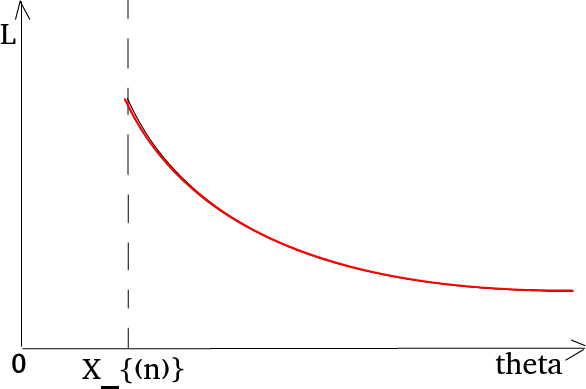
\includegraphics[width=.4\textwidth]{./pictures/v1_5.png}
  \caption{Функция правдоподобия}
  \label{fig:5}
\end{figure}

\addcontentsline{toc}{section}{Вариант 2}
\section*{Вариант 2}

\subsubsection*{1}

\textit{Задание.}
Средняя прибыль магазина за день составляет $10000$ грн.,
среднее квадратическое отклонение прибыли равно $2000$ грн.
Найдите наименьшее $n$ такое,
что с вероятностью $0.97$ прибыль магазина за $n$ дней будет не меньше чем $100000$ грн.

\textit{Решение.} Обозначим через $ \xi_n$ прибыль магазина за $n$-й день.
Тогда
$$S =
  \xi_1 + \dotsc + \xi_n$$
является прибылью магазина за $n$ дней.
Чтобы найти такое $n$, что
$$P \left( S \geq 100000 \right) =
  0.97,$$
воспользуемся аппроксимацией нормальным распределением:
$$P \left( S \geq 100000 \right) =
  P \left( \frac{S - MS}{ \sqrt{DS}} \geq \frac{100000 - MS}{ \sqrt{DS}} \right) =
  1 - \Phi_t \left( \frac{MS - 100000}{ \sqrt{DS}} \right),$$
где $ \Phi_t$ --- функция распределения стандартного нормального распределения.
Значит находит $n$ из условия
$$ \Phi_t \left( \frac{MS - 100000}{ \sqrt{DS}} \right) =
  0.03.$$
Воспользовавшись таблицей значений функции $ \Phi_t$, находим, что
$$ \frac{MS - 100000}{ \sqrt{DS}} =
  1.88.$$
По условию
$$MS = n \cdot M \xi_1 = n \cdot 10000, \,
  \sqrt{DS} = \sqrt{n \cdot 2000^2} = \sqrt{n} \cdot 2000$$
и значит $10n - 100 = 2 \cdot 1.88 \sqrt{n}$, откуда
$$ \sqrt{n} =
  \frac{2 \cdot 1.88 + \sqrt{ \left( 2 \cdot 1.88 \right)^2 + 4000}}{2 \cdot 10} =
  \frac{2 \cdot 1.88 + 63.36}{20} =
  3.36,$$
и $n = \left( 3.36 \right)^2 = 11.29$, то есть наименьшее $n = 12$.

\subsubsection*{2}

\textit{Задание.}
Пусть $X_1, \dotsc, X_n$ --- выборка из распределения $F$ и $ \nu_n$ ---
количество элементов выборки, которые попали в полуинтервал $ \left( a, b \right] $, где $a < b$ ---
фиксированные числа.
Докажите, что статистика
$$ \frac{ \nu_n}{n}$$
является несмещённой состоятельной оценкой разности $F \left( b \right) - F \left( a \right) $.

\textit{Решение.} Для того, чтобы доказать, что статистика
$$ \frac{ \nu_n}{n}$$
является несмещённой оценкой разности $F \left( b \right) - F \left( a \right) $,
необходимо проверить выполнение условия
$$M \frac{ \nu_n}{n} =
  F \left( b \right) - F \left( a \right).$$
Находим математическое ожидание статистики
$$M \frac{ \nu_n}{n} =
  M \frac{ \sum \limits_{i = 1}^n \mathbbm{1} \left\{ X_i \in \left( a, b \right] \right\} }{n} =
  \frac{1}{n} \cdot
  M \sum \limits_{i = 1}^n \mathbbm{1} \left\{ X_i \in \left( a, b \right] \right\} =
  M \mathbbm{1} \left\{ X_1 \in \left( a, b \right] \right\}.$$
Разбиваем на разность двух вероятностей
$$M \mathbbm{1} \left\{ X_1 \in \left( a, b \right] \right\} =
  P \left( X_1 \leq b \right) - P \left( X_1 < a \right) =
  F \left( b \right) - F \left( a \right).$$

Таким образом,
$$M \frac{ \nu_n}{n} =
  F \left( b \right) - F \left( a \right),$$
а значит, статистика
$$ \frac{ \nu_n}{n}$$
является несмещённой оценкой разности $F \left( b \right) - F \left( a \right) $.

Чтобы доказать состоятельность, нужно найти предел по вероятности статистики
$$ \frac{ \nu_n}{n}$$
при $n \to \infty $.
Поскольку случайные величины
$ \mathbbm{1} \left\{ X_1 \in \left( a, b \right] \right\}, \dotsc,
  X_n \in \left( a, b \right] $
являются независимыми одинаково распределёнными случайными величинами с конечным первым моментом,
то согласно с законом больших чисел
$$ \frac{1}{n} \cdot
  \sum \limits_{i = 1}^n
    \mathbbm{1} \left\{ X_i \in \left( a, b \right] \right\} \overset{P}{ \rightarrow}
  M \mathbbm{1} \left\{ X_1 \in \left( a, b \right] \right\}, \,
  n \to \infty,$$
а тогда при $n \to \infty $ выполняется
$$ \frac{ \nu_n}{n} \overset{P}{ \rightarrow }
  M \mathbbm{1} \left\{ X_1 \in \left( a, b \right] \right\} =
  F \left( b \right) - F \left( a \right).$$

Значит, статистика
$$ \frac{ \nu_n}{n}$$
является состоятельной оценкой разности $F \left( b \right) - F \left( a \right) $.

\subsubsection*{4}

\textit{Задание.}
Пусть $X_1, \dotsc, X_n$ ---
выборка объёма $n \geq 5$ из распределения Пуассона с параметром $ \lambda $.
Для какого параметра $ \theta \left( \lambda \right) $ статистика
$$ \theta_n^* =
  X_1 X_2 X_3 X_4 X_5$$
является несмещённой оценкой?
Является ли $ \theta_n^*$ состоятельной оценкой того же параметра?

\textit{Решение.}
$$M \theta_n^* =
  \theta \left( \lambda \right) =
  M \left( X_1 X_2 X_3 X_4 X_5 \right) =
  MX_1 \cdot MX_2 \cdot MX_3 \cdot MX_4 \cdot MX_5 =
  \left( MX_1 \right)^5.$$
Так как выборка имеет распределение Пуассона, то
$$ \left( MX_1 \right)^5 =
  \lambda^5.$$

Поскольку $ \theta_n^*$ не зависит от $n$,
оценка $ \theta_n^*$ не является состоятельной для $ \lambda^5$.

\addcontentsline{toc}{chapter}{Занятие 10. Интервальное оценивание параметров.
                              Доверительные интервалы}
\chapter*{Занятие 10. Интервальное оценивание параметров. Доверительные интервалы}

\addcontentsline{toc}{section}{Контрольные вопросы и задания}
\section*{Контрольные вопросы и задания}

\subsubsection*{Приведите определение доверительного интервала с уровнем значимости $ \alpha $,
                ассимпточисеского деверительного интервала с уровени значимости $ \alpha $.}

Имеем семейство распределений $F_{ \theta }$,
зависящее от параметра $ \theta \in \Theta \subset \mathbb{R}$.
Имеем выборку $X_1, \dotsc, X_n$ из распределения $F_{ \theta }$.

Есть две статистики: $T_1$ и $T_2$ такие, что $T_1 \leq T_2$ почти наверное,
то есть это некоторый случайный интервал $ \left[ T_1, T_2 \right] $.
Задаём число $ \alpha \in \left( 0, 1 \right) $, как правило $ \alpha \ll 1$.

Промежуток $ \left[ T_1, T_2 \right] $ ---
это доверительный интервал для $ \theta $ с уровнем доверия $ \alpha $,
если
$ \forall \theta \in \Theta: \,
  P_{ \theta } \left( T_1 \leq \theta \leq T_2 \right) \geq 1 - \alpha $.

Интервал $ \left[ T_1, T_2 \right] $
называется асимптотическим доверительным интервалом для параметра $ \theta $ уровня доверия
$ \alpha $,
если для любого
$$ \theta \in \Theta: \,
  \lim \limits_{n \to \infty } inf \, P_{ \theta } \left( T_1 \leq \theta \leq T_2 \right) \geq
  1 - \alpha.$$

\subsubsection*{Какая статистика называется центральной?}

Функция $G \left( \vec{X}, \theta \right) $ называется центральной статистикой,
если выполняется ряд требований:
\begin{enumerate}
  \item $G \left( \vec{X}, \cdot \right) $ --- функция второго аргумента ---
  строго монотонна и непрерывна (либо строго возрастает, либо строго убывает);
  \item $G \left( \vec{X}, \theta \right) $ имеет известное распределение,
  не зависящее от $ \theta $.
\end{enumerate}

\subsubsection*{Как с помощью центральной статистики построить доверительный интервал с заданным
                уровнем доверия?}

Пусть $G$ --- центральная статистика.
Распределение $G$ --- известно.

Следовательно, по $ \alpha $ можно указать такие числа $a_1 < a_2$, что имеет место следующее:
$P \left\{ a_1 \leq G \left( \vec{X}, \theta \right) \leq a_2 \right\} \geq
  1 - \alpha $.

Считаем, что $G \left( \vec{X}, \cdot \right) $ возрастает.
Тогда это равносильно тому,
что
$$P_{ \theta } \left\{
    G^{-1} \left( \vec{X}, a_1 \right) \leq \theta \leq G^{-1} \left( \vec{X}, a_2 \right)
  \right\}
  \geq 1 - \alpha.$$
Эти границы $G^{-1} \left( \vec{X}, a_1 \right), \, G_2^{-1} \left( \vec{X}, a_2 \right) $ ---
доверительный интервал.

\addcontentsline{toc}{section}{Аудиторные задачи}
\section*{Аудиторные задачи}

\subsubsection*{10.3}

\textit{Задание.}
По выборке $X_1, \dotsc, X_n$ из нормального распределения $N \left( a, \sigma^2 \right) $
постройте доверительные интревалы для параметров распределения, если:
\begin{enumerate}[label=\alph*)]
  \item $a$ неизвестный параметр, $ \sigma^2$ --- известный;
  \item $ \sigma^2$ неизвестный параметр, $a$ --- известный.
\end{enumerate}

\textit{Решение.} С помощью этих распределений можно строить доверительный интервал:
$$ \begin{cases}
    \frac{ \sqrt{n} \left( \overline{X} - a \right) }{ \sigma } \sim N \left( 0, 1 \right), \\
    \frac{ \left( n - 1 \right) \hat{ \sigma^2}}{ \sigma^2} \sim \chi_{n - 1}^2, \\
    \frac{ \sqrt{n} \left( \overline{X} - a \right) }{ \hat{ \sigma }} \sim t_{n - 1}.
  \end{cases}$$

\begin{enumerate}[label=\alph*)]
  \item Используем первое
  $$ \xi =
    \frac{ \sqrt{n} \left( \overline{X} - a \right) }{ \sigma } \sim
    N \left( 0, 1 \right).$$

  Если задан уровень доверия $ \alpha $, по таблице можем найти
  $$P \left( \xi \geq u_{ \frac{ \alpha }{2}} \right) =
    \frac{ \alpha }{2} =
    \Phi \left( u_{ \frac{ \alpha }{2}} \right).$$

  Плотность имеет вид колокольчика,
  поэтому
  $$P \left( \xi \leq - u_{ \frac{ \alpha }{2}} \right) =
    P \left( \xi \geq u_{ \frac{ \alpha }{2}} \right).$$
  Это значит,
  что
  $P \left( -u_{ \frac{ \alpha }{2}} \leq \xi \leq u_{ \frac{ \alpha }{2}} \right) =
    1 - \alpha $.
  Следовательно, выбираем
  $$ \frac{ \alpha }{2}$$
  так, чтобы в сумме было $ \alpha $.

  Подставляем значение случайной величины
  $$P \left(
      -u_{ \frac{ \alpha }{2}} \leq \frac{ \sqrt{n} \left( \overline{X} - a \right) }{ \sigma } \leq
      u_{ \frac{ \alpha }{2}}
    \right) =
    1 - \alpha.$$
  Нужно найти отрезок для $a$.
  Получаем
  \begin{equation*}
    \begin{split}
      P \left(
        -u_{ \frac{ \alpha }{2}} \cdot \frac{ \sigma }{ \sqrt{n}} - \overline{X} \leq -a \leq
        u_{ \frac{ \alpha }{2}} \cdot \frac{ \sigma }{ \sqrt{n}} - \overline{X}
      \right) = \\
      = P \left(
        u_{ \frac{ \alpha }{2}} \cdot \frac { \sigma }{ \sqrt{n}} + \overline{X} \geq a \geq
        \overline{X} - u_{ \frac{ \alpha }{2} \cdot \frac{ \sigma }{ \sqrt{n}}}
      \right) =
      1 - \alpha,
    \end{split}
  \end{equation*}
  где
  $$u_{ \frac{ \alpha }{2}} \cdot \frac { \sigma }{ \sqrt{n}} + \overline{X}$$
  --- статистика $T_2$, а
  $$ \overline{X} - u_{ \frac{ \alpha }{2} \cdot \frac{ \sigma }{ \sqrt{n}}}$$
  --- статистика $T_1$.

  Получаем доверительный интервал
  $$ \left[ T_1, T_2 \right] =
    \left[
      \overline{X} - u_{ \frac{ \alpha }{2} \cdot \frac{ \sigma }{ \sqrt{n}}},
      u_{ \frac{ \alpha }{2}} \cdot \frac { \sigma }{ \sqrt{n}} + \overline{X}
    \right];$$
  \item распределение $ \chi^2$ сосредоточено на полуинтервале $ \left[ 0, + \infty \right) $,
  оно не может быть симметричным.
  Допустим,
  $$ \xi =
    \frac{ \left( n - 1 \right) \hat{ \sigma^2}}{ \sigma^2} \sim
    \chi_{n - 1}^2.$$

  Имеем вероятность
  $P \left\{ \chi_{n - 1}^2 < x_{n - 1} \left( \alpha \right) \right\} =
    \alpha \in \left( 0, 1 \right) $.

  Из рисунка \ref{fig:103} видно, что
  $$P \left( \xi \leq y_1 \right) =
    \frac{ \alpha }{2}$$
  и
  $$P \left( \xi \geq y_2 \right) =
    \frac{ \alpha }{2}.$$

  \begin{figure}[h!]
    \centering
    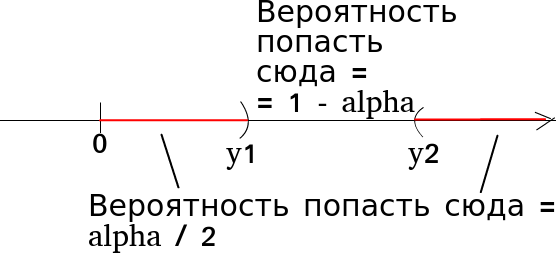
\includegraphics[width=.4\textwidth]{./pictures/10_3.png}
    \caption{Вероятность попадания в отрезок}
    \label{fig:103}
  \end{figure}

  Функция распределения будет иметь вид, показанный на рисунке \ref{fig:1031}.

  \begin{figure}[h!]
    \centering
    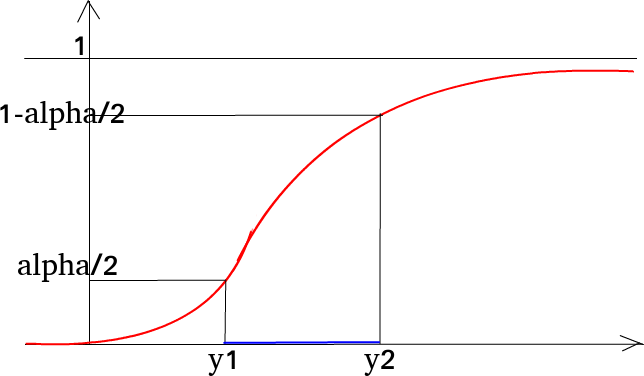
\includegraphics[width=.4\textwidth]{./pictures/10_3_1.png}
    \caption{Функция распределения}
    \label{fig:1031}
  \end{figure}

  $P \left( \xi \geq y_1 \wedge \xi \leq y_2 \right) = 1 - \alpha $.

  Подставляя вместо $ \xi $ выражение,
  можем определить интервал
  $$P \left( y_1 \leq \xi \leq y_2 \right) =
    1 - \alpha,$$
  то есть
  $$P \left\{ y_1 \leq \frac{ \left( n - 1 \right) \hat{ \sigma^2}}{ \sigma^2} \leq y_2 \right\} =
    1 - \alpha.$$

  Выражем пределы для нужной величины
  $$P \left\{
      \frac{1}{ \left( n - 1 \right) \hat{ \sigma^2}} \leq \frac{1}{ \sigma^2} \leq
      \frac{y_2}{ \left( n - 1 \right) \hat{ \sigma^2}}
    \right\} =
    1 - \alpha,$$
  получаем
  $$P \left\{
      \frac{ \left( n - 1 \right) \hat{ \sigma^2}}{y_2} = T_1 \leq
      \frac{ \left( n - 1 \right) \hat{ \sigma^2}}{y_1} = T_2
    \right\} =
    1 - \alpha.$$

  Получили выражение $P \left( T_1 \leq \sigma^2 \leq T_2 \right) = 1 - \alpha $, значит,
  $ \left[ T_1, T_2 \right] $ -- доверительный интеравал.
\end{enumerate}

\addcontentsline{toc}{section}{Домашнее задание}
\section*{Домашнее задание}

\addcontentsline{toc}{chapter}{Занятие 12. Проверка параметрических гипотез.
                              Критерий Неймана-Пирсона}
\chapter*{Занятие 12. Проверка параметрических гипотез. Критерий Неймана-Пирсона}

\addcontentsline{toc}{section}{Контрольные вопросы и задания}
\section*{Контрольные вопросы и задания}

\subsubsection*{Что называется статистической гипотезой?}

Статистическая гипотеза --- предположение о виде распределения и свойствах случайной величины,
которое можно подтвердить или опровергнуть применением статистических методов к данным выборки.

\subsubsection*{Какую гипотезу называют основной, альтернативной, простой, сложной?}

Нулевая гипотеза --- гипотеза, подлежащая проверке.
Альтернативная гипотеза --- каждая допустимая гипотеза, отличная от нулевой.
Нулевую гипотезу обозначают $H_0$, альтернативную ---
$H_1$ (от Hypothesis --- <<гипотеза>> (англ.)).

Простой гипотезой называют предположение, состоящее в том,
что неизвестная функция $F \left( t \right) $
отвечает некоторому совершенно конкретному вероятностному распределению.

Сложной гипотезой называют предположение о том,
что неизвестная функция $F \left( t \right) $ принадлежит некоторому множеству распределений,
состоящему из более чем одного элемента.

\subsubsection*{Что такое статистический критерий?}

Статистический критерий --- строгое математическое правило,
по которому принимается или отвергается та или иная статистическая
гипотеза с известным уровнем значимости.

\subsubsection*{Что такое уровень занчимости критерия для проверки статистической гипотезы?}

Можно отвергнуть гипотезу $F_1$, когда она будет верна.
В случае простой гипотезы $F_1$ вероятность ошибки равна  $P_{F_1} \left( \vec{X} \in D \right) $.
Эту вероятность называют уровнем значимости статистического критерия.

\subsubsection*{Какое множество называют критическим для проверки статистической гипотезы?}

Критическая область --- это совокупность значений статистики, которые <<говорят>>,
что нулевую гипотезу следует отвергнуть.

\subsubsection*{В чём состоит ошибка первого рода, второго рода?}

$1 - \alpha = P \left( H_1 \; \middle| \; H_0 \right) $ --- ошибка первого рода.
Означает, что отклонили нулевую гипотезу в то время, как на самом деле она истинна.

$ \beta = P \left( H_0 \; \middle| \; H_1 \right) $ --- ошибка второго рода.
Это означает принять нулевую гипотезу, которая на самом деле ложна.

\subsubsection*{Что называют мощностью критерия?}

$1 - \beta $ --- мощность критерия.

\subsubsection*{Сформулируйте критерий согласованности Колмогорова,
                критерий согласованности $ \chi^2$ Пирсона, лемму Неймана-Пирсона}

\textit{Критерий Колмогорова-Смирнова.}
Если $F$ --- непрерывное распределение,
то
$ \sqrt{n} \cdot
  \sup \limits_{ \mathbb{R}} \left[ F_n \left( x \right) - F \left( x \right) \right] \approx
  D_{ \theta }$
--- известное распределение.

\textit{Критерий Пирсона (критерий согласия $ \chi^2$).} Есть выборка $X_1, \dotsc, X_n$.
Имеет ли оа распределение $F$?
Попробуем устроить дискретную процедуру.
Разбиваем интервал возможных значений выборки на $N$ полуинтервалов (чисел, частей) ---
рис. \ref{fig:12}.

\begin{figure}[h!]
  \centering
  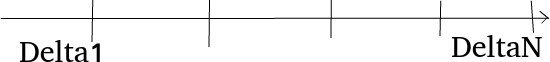
\includegraphics[width=.4\textwidth]{./pictures/12.png}
  \caption{Возможные значения выборки}
  \label{fig:12}
\end{figure}

Обозначим через $p_i = P_F \left( X_1 \in \Delta_i \right) > 0$.

Количество элементов выборки, которые попали в $ \Delta_i$, обозначим через
$$ \nu_i =
  \sum \limits_{k = 1}^n \mathbbm{1}_{ \Delta_i} \left( X_k \right).$$
Рассмотрим сумму
$$ \sum \limits_{i = 1}^n \frac{ \left( \nu_i - np_i \right)^2}{np_i} \approx
  \chi_{n - 1}^2$$
при $n \to \infty $ (после применения центральной предельной теоремы).

Все $ \nu_i$ в сумме дают $n$, следовательно, есть связь,
то есть $ \left( n - 1 \right) $-на степень свободы.

Так происходит, если угадали $p_i$, иначе --- выражение быстро растёт.

\textit{Лемма Неймана-Пирсона.}
$D_{C_{ \alpha }}$ --- оптимально, то есть для произвольной $D$,
такой что $P_{F_1} \left( D^C \right) = \alpha $, оказывается,
что $P_{F_2} \left( D \right) = P_{F_2} \left( D_{C_{ \alpha }} \right) $, то есть утверждается,
что множество уровня является оптимальным.

\addcontentsline{toc}{section}{Аудиторные задачи}
\section*{Аудиторные задачи}

\addcontentsline{toc}{section}{Домашнее задание}
\section*{Домашнее задание}


\end{document}
